\documentclass[a4paper]{amsbook}%
%\usepackage[scaled]{helvet}
%\renewcommand*\familydefault{\sfdefault} 
\usepackage{rawfonts}
\usepackage[top=1.25in,bottom=1.3in,left=1.25in,right=1.25in]{geometry}
\usepackage{fp}
%\usepackage[body={6.0in, 8.2in},left=1.25in,right=1.25in]{geometry}  
\usepackage{amsmath,amssymb}             % AMS Math 
\usepackage{pstricks, pst-node,pst-tree}
\usepackage{graphicx}
\usepackage{ntabbing}
\usepackage{subfigure}
% a list with labelled items
\newenvironment{mylist}
{\begin{list}
	{}
	{
		\setlength{\topsep}{0.5em}
		\setlength{\partopsep}{0pt}
		\setlength{\parskip}{0pt}
		\setlength{\parsep}{0pt}
		\setlength{\itemsep}{\topsep}	% space between items
		\setlength{\labelwidth}{1em}
		\setlength{\labelsep}{5pt}          % between label and text
		\setlength{\itemindent}{\labelsep}    % indent start of item paragraph
		\setlength{\listparindent}{1em}
		\setlength{\leftmargin}{1.5em}    % all items
		\setlength{\rightmargin}{0pt}    % all items
		\renewcommand\makelabel[1]{$*$ \myterm{##1}.}
	}
}
{\end{list}}

% a list without labelled items
\newenvironment{mydesclist}
{\begin{list}
	{}
	{
		\setlength{\topsep}{0.5em}
		\setlength{\partopsep}{0pt}
		\setlength{\parskip}{0pt}
		\setlength{\parsep}{0pt}
		\setlength{\itemsep}{\topsep}	% space between items
		\setlength{\labelwidth}{1em}
		\setlength{\labelsep}{0pt}          % between label and text
		\setlength{\itemindent}{\labelsep}    % indent start of item paragraph
		\setlength{\listparindent}{1em}
		\setlength{\leftmargin}{1.5em}    % all items
		\setlength{\rightmargin}{0pt}    % all items
		\renewcommand\makelabel[1]{$*$ \sl{##1}}
	}
}
{\end{list}}

%pseudo code
\newenvironment{code} 
	{\begin{sffamily}
	\begin{tabbing}} 
	{\end{tabbing}
	\end{sffamily} }

%references
\newcommand{\reftab}[1]{Table \ref{tab:#1}}
\newcommand{\refeq}[1]{Equation \ref{eq:#1}}
\newcommand{\refsec}[1]{Section \ref{sec:#1}}
\newcommand{\reffig}[1]{Figure \ref{fig:#1}}
\newcommand{\refalg}[1]{Figure \ref{alg:#1}}
\newcommand{\refline}[1]{line \ref{line:#1}}
\newcommand{\refdef}[1]{Definition \ref{def:#1}}

% special words and phrases
\newcommand{\etal} {{\it et. al.} }
\newcommand{\chapterintro} {\it \small}
\newcommand{\mytdist} {{\sl t}-distribution}
\newcommand{\myFdist} {{\sl F}-distribution}
\newcommand{\myatdist} {{\sl *t}-distribution}
\newcommand{\myFvalue} {{\sl F}-value}
\newcommand{\mytvalue} {{\sl t}-value}
\newcommand{\svar}[1]{s^2_{\mbox{\tiny #1}}} % sample variance
\newcommand{\var}[1]{\sigma_{\mbox{\tiny #1}}^{2}}  % variance
\newcommand{\mean}[1]{\overline{X}_{\mbox{\tiny #1}}}  % sample mean is X
\newcommand{\Fdist}[3]{{\it F}^{(#1)}_{#2,#3}} % F-Distribution
\newcommand{\tdist}[2]{{\it t}^{(#1)}_{#2}} % t-Distribution
\newcommand{\header}[1]{\subsubsection{#1}}
\newcommand{\prob}[1]{\mbox{Pr}(#1)} % probability
\newcommand{\myterm}[1]{{\sl #1}}  % a new term introduced in the text
\newcommand{\mygame}[1]{\textsc{#1}}  % commands used for game names
\newcommand{\myprogram}[1]{\textbf{\it #1}} % the name of a program 
\newcommand{\myset}[1]{{\bf #1}} % a symbol representing a set
\newcommand{\myrel}[1]{{\bf #1}} % a symbol representing a relation
\newcommand{\mydom}[1]{\mathbb{#1}} % a defined set
\newcommand{\mysetof}[1]{\{e \; | \; e \in #1\}} % a symbol 
\newcommand{\mytabheader}[1]{\bf #1} % heading in a tabular
\newcommand{\myheading}[1]{\par\vspace{10pt}\noindent{\bf #1}
\newline\par}	% essentially a  \subsubsubsection
\newcommand{\merge}{\oplus}
\newcommand{\myfrac}[2] { \left(\begin{array}{c} #1 \\#2\end{array}\hspace{-5pt}\right) }
% Symbols used
\newcommand{\pbest}[1]{\mbox{\it pbest}(#1)}
\newcommand{\pbestt}[1]{\mbox{\it pbest}_t(#1)}
\newcommand{\gbest}[1]{\mbox{\it gbest}(#1)}
\newcommand{\lbest}[1]{\mbox{\it lbest}(#1)}
\newcommand{\lbestt}[1]{\mbox{\it lbest}_t(#1)}
\newcommand{\neighbours}[1]{\myset N_{\vec{#1}}}
	% component of vector
\newcommand{\comp}[2]{{#1}[#2]}   
	% velocity of particle
\newcommand{\vel}[1]{v(#1)}   
\newcommand{\velcomp}[2]{v(#1)[#2]}   
\newcommand{\velepoch}[2]{v_{#2}(#1)}   
	% component of velocity of particle
\newcommand{\velepochcomp}[3]{v_{#2}(#1)[#3]}    
\newcommand{\mywin}{{\cal W}}
\newcommand{\mylose}{{\cal L}}
\newcommand{\mydraw}{{\cal D}}
\newcommand{\myor}{\vee}
\newcommand{\myand}{\;\wedge\;}
\newcommand{\myunion}{\cup}
\newcommand{\myintersect}{\cap}
\newcommand{\myst}{\; | \;} % such that
\newcommand{\mysquare}[2]{(#1,#2)} % file, rank
\newcommand{\mysquares}{\mydom{S}}
\newcommand{\mypieces}{\mydom{O}}
\newcommand{\mycardinalities}{\mydom{C}}
\newcommand{\myatoms}{\mydom{A}}
\newcommand{\mypositions}{\mydom{P}}
\newcommand{\myplacements}{\myrel{P}}
\newcommand{\myints}{\mathbb Z}
\newcommand{\mynaturals}{\mathbb N}
\newcommand{\mytrue}{\mbox{\it true}}
\newcommand{\myfalse}{\mbox{\it false}}

% help with equations
\newcommand{\mywhere}{\noindent where}
\newcommand{\myarg}{\newline\indent\indent}
\newcommand{\myreal}{{\mathbb R}}
\newcommand{\mymap}{\rightarrow}
\newcommand{\mywff}{\textit{wff}}
\newcommand{\mywffs}{{\it wff}s}

\newcommand \myprint [1] {\FPround \fpr {#1} 6 \FPprint \fpr}
\newcommand \myeval [1] {\FPeval \val {#1} \FPround \rval \val 6 \FPprint \rval}

% New Environments
% \newtheorem{mydef}{Definition}[section]
\newcounter{mydef}[chapter]
\newenvironment{mydef}[1] 
{	
	\stepcounter{mydef}
	\par
%	\bigskip
	{\bf Definition \arabic{chapter}.\arabic{mydef}: \sl{#1}.}
%	\begin{minipage}[c]{315pt}
}
{ 	
%	\end{minipage}
%	\bigskip
}

% algorithms must be encapsulated in figures
\newenvironment{algorithm}[3] 
% the first parameters is the name
% the second parameter describes the input
% the third parameter describes the output
% the body of the environment contains the pseudo code  lines are terminated with \\ and \> is used to indent
{
\small
\begin{tabular} [t] {rp{60ex}}
\hline
\\
	{\it Algorithm} & #1 \\
	{\it Input} & #2  \\
	{\it Output} & #3 \\
\end{tabular}
	\begin{sffamily}		
	\small
	\begin{ntabbing}

	\reset
	123\=123\=123\=123\=123\=123\=\kill
	
}{
	\end{ntabbing}
	\end{sffamily}
}

% Name of a new parameter function
\newcommand{\paramfun} {\pi_{\arabic{equation}}}
% Commands to draw a board
\newcommand{\mycenter} [1] {\parbox{0.75em}{\centering{#1}}}
\newcommand{\myrowa} [5] {\hline \textbf{#1}& \mycenter{#2}&
&\mycenter{#3}&&\mycenter{#4}& &\mycenter{#5}& }
\newcommand{\myrowb} [5] {\hline \textbf{#1}& &\mycenter{#2}& &\mycenter{#3}&
&\mycenter{#4}& &\mycenter{#5}}
\newcommand{\myrefboard} {Board diagram \arabic{section}.\arabic{board}}
\newcommand{\myrefstepboard} {\refstepcounter{board} \myrefboard}
\newcommand{\myboard} [8]
{
\begin{center}
\small
\begin{tabular}[!ht] {c|c|c|c|c|c|c|c|c|}
\multicolumn{9}{c}{Active (o)} \\
 \myrowb {8}   #1 \\ 
 \myrowa {7}   #2 \\ 
 \myrowb {6}   #3 \\ 
 \myrowa {5}   #4 \\ 
 \myrowb {4}   #5 \\ 
 \myrowa {3}   #6 \\ 
 \myrowb {2}   #7 \\
 \myrowa {1}   #8 \\
\hline
  &\textbf{1}&\textbf{2}& \textbf{3} & \textbf{4} & \textbf{5} & \textbf{6}  & \textbf{7} & \textbf{8} \\
\multicolumn{9}{c}{Passive (x)} \\
\end{tabular}
\end{center}
\begin{flushright}
\myrefboard \\
\end{flushright}
}

\newcounter {board} [section]

% Usage: \
%		statsTable  {label} {caption} {body}
\newcommand{\statsTable} [4]
{
	\begin{table} [h!]
	\small
	\centering
	\begin{tabular}{|c|c|c|c|c|}
	\hline
	S & $\mean S$ & $\svar S$ & Max & Min \\
	\hline
	#3
	\hline
	\end{tabular}
	\caption{#2}
	\label{tab:#1}
	\end{table}
}
\usepackage{xcolor}

\newcommand{\ui}[1]{\textit{#1}}
\newcommand{\example}[2]{\item {\it #1:} \newline \code{#2}  } 
\newcommand{\na}[0]{Not applicable}

\usepackage{graphicx}
\usepackage{hyperref}
%\usepackage[top=2cm, bottom=2cm, left=3cm, right=3cm]{geometry}
\usepackage{subfigure}
\usepackage{enumitem}
\usepackage{longtable}
\usepackage{url}
\usepackage{amsmath,amssymb} 
\usepackage{amsthm}
\usepackage{microtype}
\newtheorem{definition}{Definition}
\title{A learning framework for Zero knowledge agents}
\author{Willem Duminy}
\begin{document}

\maketitle
\newpage
\tableofcontents
\definecolor{light-gray}{gray}{0.8}
\hypersetup{%
	citebordercolor=white,
  linkbordercolor=white,
	urlbordercolor=light-gray,
}
\newcommand{\mytermmark}[1]{{\sc #1}} 
\newcommand{\myterm}[1]{\hyperlink{#1}{\sc #1}}
\newcommand{\myterms}[1]{\hyperlink{#1}{\sc #1s}}
\newcommand{\refterm}[1]{\myterm{#1} (p. \pageref{def:#1})}
\newcommand{\refterms}[1]{\myterms{#1} (p. \pageref{def:#1})}
\newcommand{\wikiref}[1]{(see \href{http://en.wikipedia.org/wiki/#1} {wikipedia})}
% this is a 'template command' do not use directly
\newcommand{\mydefT}[3]{
\begin{definition}[#1]  \label{def:#1} \hypertarget{#1}
{#2} #3
\end{definition}

} 
% simple definition: mydefs name definition
\newcommand{\mydefs}[2]{\mydefT{#1}{ }{#2}}
% definition with context: mydefc name context definition
\newcommand{\mydefc}[3]{\mydefT{#1}{[#2]}{#3}}
\chapter{Two-player games}
\label{chap:two-player}
{ \chapterintro
This chapter reviews fundamental two-player definitions and concepts used in chapters that follow.  Furthermore, the reasons for using games in research and the properties that are typically used to classify two-player games are explored. Game convergence is such a property, and a new, more general definition of this property extends work done previously in this regard.  Throughout the chapter, the perspective remains on the influence the presented material might have on the definition of a learning framework.}

\section{Introduction}
\label{sec:two-player-intro}
For centuries, two-player games continued to be a source of amusement to the human race.  This lasting interest can surely by attributed, at least in part, to the variety of games available.  From this variety many diverse strategies arise, such that a strategy that often wins any particular game is seldom transferable to another game. Because every game is a different kind of puzzle, many researchers found it best to choose a specific game as subject. Others, like David Fogel \cite{fogel:networks,fogel:edge,fogel:chess}  started with simpler games and turned their attention to more complex games as the research progressed. 

An automated learning process that can be applied to all two-player games has not yet been discovered, and it is likely to remain unattainable for some time. This general problem can be divided into smaller steps by considering layers of knowledge. Each layer builds on the knowledge obtained by the previous layer.  At the bottom layer, there is the \myterm{playing agent} that has the knowledge of how to play the game.  The next layer is the \myterm{learning agent}; it needs to know how to play, but also has knowledge on how to learn to play better. The third layer is the \myterm{learning framework}; it extends the knowledge of how to learn a particular game to define a process by which other games of the same class can be learned.  Finally, at the top of the stack, the \myterm{two-player game agent} automates the improvement of learning frameworks and the development of new learning frameworks for other classes of two-player games. The current work contributes to the research conducted at the second and third layers. 
 
At the start of this chapter, \refsec{concepts-and-terms} provides background on the terminology and the concepts pertaining to automated game-playing. Then, \refsec{motives}  reviews the most important drivers that motivate researchers to spend their time on the subject of games. Game playing cannot be automated without search, and \refsec{knowledge-and-search} highlights this important facet and considers the influence of search on the learning framework. \refsec{properties} addresses the classification problem by considering a few critical properties of two-player games.  The final section of this chapter provides a summary of the notable conclusions.  

% must be the first section because the other sections depend upon the definitions contained here
\section{Game playing terminology and concepts}
\label{sec:concepts-and-terms}

Fundamentally, a game is a set of rules.  These rules define how the game starts, what the legal moves are,  when the game ends and who the winner is.  

\mydefs{two-player game} {A game where two participants compete in a contest determined by the game rules.} 

In an abstract sense,  game rules describe allowable changes to the \myterm{game state}.  For board games, the game state is usually referred to as a \myterm{position}. 

\mydefs{legal position} {A game state that can be constructed by playing the game according to its rules.}

Three mutually exclusive sets cover the set of legal positions: the set of \myterm{initial positions}; the set of \myterm{middle positions} and the set of \myterm{end positions}.  A game starts with an initial position and it ends with an end position.  Any legal position not in the initial- or end position set belongs to the set of middle positions. Many popular games have only one initial position, but there are exceptions.  For instance, in  \mygame{Tournament Checkers} the initial position is determined from a balloted sequence of three moves \cite{schaeffer:solving} -- and the set of  initial positions has 144 elements. \mygame{Arimaa} starts with each player in turn arranging 16 game pieces on the nearest two ranks on a \mygame{Chess} board.  In this game there are thousands of initial positions\footnote{See http://www.arimaa.com for the \mygame{Arimaa} game rules}. 

The outcome of a match is determined from the end position.  A game in which the outcome is either a win, a lose or a draw for each player is said to have a  \myterm{restricted outcome} \cite{davis:evolve}.  The player's goal is to make moves that force the outcome towards an end-game position in which he wins. With respect to a player, the symbol $\mylose$ signifies the lose outcome, $\mydraw$ signifies the draw, and $\mywin$ signifies the win of a match.   

\mydefc{state-space} {of a game} {The set of all \myterms{legal position}.}
 
%.  This game has approximately $10^{20}$ initial positions.  


Using a position centric view, the rules of the game can be regarded as the input to a production system that starts from an initial position and produces all the legal positions that follow.  Repeating the production, level by level, results in a tree structure with the initial position as the root and end positions as leaf nodes. This tree structure is called a \myterm{game tree} and each level in the tree is called a \myterm{ply} \cite{samuel:checkers}.  The \myterm{branching factor} is a measure of the average number of child nodes. The set of all game trees with an initial position as root is called the \myterm{game forest}.  

During the game, the nodes of the game tree is traversed and a path is constructed.  This path is called a \myterm{play-line} and it starts at the root of a game tree and extends towards the leaves of the tree as the game progresses.  The \myterm{active game tree} is the tree in which the play-line is found. The \myterm{active position} is the last node in the play line.  The \myterm{past positions} are the nodes that precede the active position, and the \myterm{future lines} are all the paths in the game tree with the active position as root.  

For any given position, the \myterm{active player} is the player that must choose the next node in the play line.  The other player is called the \myterm{passive player}.  The player that is active at the first node in the play line is called the \myterm{first player} and the passive player for that node is referred to as the \myterm{second player}.


\section{Motivations for using games in research}
\label{sec:motives}
The domain of two-player games presents a scientist in the field of artificial intelligence (A.I.) with an artificial problem that has well defined rules and a definite goal.  Even though the goal and the rules are elementary, devising a strategy to win a non-trivial game is a complex task that demands the use of intelligence. These qualities of game domains has been recognised as beneficial to A.I. research since the late 1950's \cite{samuel:checkers}.      

The primary motivations for using games as a research tool support three different research objectives.  One objective aims to win tournaments and focus on creating the best player for a particular game.  Another objective aims to solve the game by producing an infallible strategy. The third objective regards games as ideal learning domains, and aims to investigate machine learning methods.

When compared to research projects conducted to create winning computer players, projects that apply games to the problem of investigating learning methods are less prevalent. There is reason to expect that a solution to the latter coincides with progress made to the former; and notable contributions have been made in this regard.  However, it is also possible for competition matches, especially public exhibitions, to stifle research progress. In \refsec{winning} the contributive as well as the prohibitive aspects of these matches are explored. The objective to solve a game is discussed in \refsec{solving}. \refsec{investigating} considers the factors that make game domains ideal for automated learning.


\subsection{Winning public tournaments}
\label{sec:winning}
Artificial intelligence is convincingly demonstrated when the behaviour of the artificial agent is understood by the audience. Therefore a game playing program that beats a human opponent is ideal for such displays. Annual tournament matches against \mygame{Chess} playing agents have been held since 1970 \cite{donskoy:grace}.  In 1992, the American Checkers Foundation and the English Draughts Association even established a Man-Machine World Championship title for \mygame{Checkers} \cite{schaeffer:solving}. The computer \mygame{Chess} match of 1997 that played off Deep Blue against Gary Kasparov (the world \mygame{Chess} champion since 1985) is arguably the most celebrated achievement in A.I. history.

The desire to perform well in the spotlight is a strong motivation:  potential returns include monetary gains, publicity and prestige. 
However, the famous Deep Blue vs. Kasparov match and other like-minded efforts had a less than expected  impact on the science of A.I.  This is partly because exhibition programs  implement techniques that many A.I. researchers regard as uninteresting.  Public exhibitions encourage small, short-term projects that focus on the player's performance, while A.I. research attempts  to find  solutions to problems that require a longer term commitment.  Some specific issues have been highlighted with regard to \mygame{Chess} programming endeavours  
\cite{donskoy:grace}:
\begin{mydesclist}
\item While they were chasing deadlines, the neglect of \mygame{Chess} programmers to sell their ideas contributed to the diminution of the esteem once enjoyed by the game of \mygame{Chess} in A.I. research.
\item Experiments conducted solely to test the strength of the player lead to a reliance on results of which the underlying theory was not always understood.  Even though a lot of research was conducted, there is little theory of \mygame{Chess} knowledge and its interactions with search.
\item High pay-off to the winner eradicates incentives for the dissemination of research results.  The tendency is to hold back on ideas to maintain a competitive edge, leaving each team to discover principles that are already known to other teams.
\end{mydesclist}

Nonetheless, the exploration and definition of methods to create champion game software has become an established field with many research challenges. Even in \mygame{Chess},  human master players currently beat the best \mygame{Chess} programs more often than not \cite{sonas:strongest}; and the next frontier is the game \mygame{Go}. Research endeavours typically focus on high performance implementations that take advantage of specific hardware architectures and multiprocessor platforms. This commendable approach is likely to reassert itself as the most important factor in the next generation of champion game playing agents.

\subsection{Solving the game}
\label{sec:solving}
A game is solved if a playing agent is available that is guaranteed to win from a position where a win can be forced.  In other words, the puzzle of winning the game against any opponent is solved.  After a game is solved, it is possible to determine whether the game is fair. 

A precise definition of what it means to solve a game is based on an irrefutable property of a game position, called the \myterm{game-theoretic value}.  This value is computed in a retrograde search that starts with the end positions in the game tree. A precise definition of the game-theoretic value follows.  

In restricted outcome games, every end position determines the outcome of the game.  For end positions this outcome is the game theoretic value. The value is an element from the \myterm{outcome set} $\mydom{O} \equiv \{\mywin,\mylose,\mydraw\}$ that designates a win ($\mywin$), lose ($\mylose$) or a draw ($\mydraw$) for the active player. For an initial and middle position the game theoretic value is $\mywin$ if it is in a play line in which the active player can force a win.  Conversely, if the passive player can force a win from a position, the game-theoretic value of that position is $\mylose$.  If neither player is able to secure a winning outcome, the position leads to a draw, and has the game-theoretic value of $\mydraw$. 

Formally, let the domain $\mydom{S}_g$ be the state-space of game $g$ and ${\bf C}_g:\mydom{S}_g \mymap \mysetof{\mydom{S}_g}$ be a set function that determines the positions that may legally follow from another.  Then, the \myterm{game-theoretic value} for the active player can be defined as the recursive function $\theta_g: \mydom{S}_g \mymap \mydom{O}$:

\begin{equation}
\label{eq:solve}
\theta_g(s)  =  \left\{
\begin{array}{l}
\mbox{For the base step ($s$ is an end position):}\\
	\left\{
	\begin{array} {ll}
		\mylose & $if the active player of $s$ loses$ \\
		\mywin &  $if the active player of $s$ wins$ \\
	    \mydraw & $if $s$ is a draw position$\\
	\end{array}		
	\right.
	\\
\\
\\
\mbox{For the recursive step ($s$ is not an end position):}\\
	\left\{
	\begin{array} {lcl}
		\mylose & $if$ & \exists e \in {\bf C}_g(s) \myst  \theta_g(e) = \mywin  \\
		\mywin & $if$ & \forall e \in {\bf C}_g(s) \;,\;  \theta_g(e) = \mylose  \\
	    \mydraw & $if$ &  (\nexists e \in 
	                      {\bf C}_g(s) \myst  \theta_g(e) = \mywin)\; \myand \\                         & &   
	                      (\exists 
	                      e \in {\bf C}_g(s) \myst  \theta_g(e) = \mydraw)
	\end{array}		
	\right.
\end{array}
\right.
\end{equation}

Although the computation is simple, the size of the state space for non-trivial games makes it impossible to compute the game-theoretic value for all positions.  However, as the availability of faster hardware and larger memory sizes increases it becomes slightly easier to compute these values.  

From the game-theoretic value follows a definition in Allis \cite{allis94}:  A game is \myterm{strongly solved} when the game-theoretic value for both players can be determined for any legal position using reasonable computing resources.  Without the reference to ``reasonable resources", any two-player game is strongly solved, because the game-theoretic value can simply be determined using \refeq{solve}. A number of games have been strongly solved: these include \mygame{Connect-four}, \mygame{Qubic}, \mygame{Nine  Men's Morris}, \mygame{Go-Moku} and \mygame{Awari} \cite{vandenherik:games}. Because of the end-game database, Chinook strongly solved the end-game of \mygame{Checkers} \cite{schaeffer:reexamination}.

The term \myterm{perfect play} is used to describe a move decision that ensures an outcome that is no less than the game theoretic value.  The weakness of perfect play is that once it has been determined that a position has been reached with an outcome of a draw, there is no reason to continue playing.  But, humans are not perfect players, and under draw conditions, the playing agent would do well to select a move that maximises the likelihood that the opponent makes an error.  Schaeffer \cite{schaeffer:solving} highlights this situation by introducing a stronger definition: A game is \myterm{ultra strongly solved}  when it is strongly solved and a strategy is known that improves the chance of achieving more than the game-theoretic value against a fallible opponent.  

This aim to solve a game ultra strongly is interesting, but in practice the playing agent needs a fallible opponent that plays very close to perfection before this ability can be tested.  Even amongst master players, these individuals are extremely rare.  

\subsection{Investigating methods in machine learning}
\label{sec:investigating}
Arthur Samuel was the first to use game playing to investigate machine learning methods. He felt compelled to win over his contemporaries to the notion that a computer program can learn \cite{samuel:checkers}.  With this end in mind, he set out to develop a \mygame{Checkers} program that uses previous experience to make a move decision.  As attested by the praise of another prominent A.I. researcher of the time, Marvin Minsky, Samuel's program proved to be a convincing demonstration of machine learning \cite{minsky:steps}.  


There are four aspects of game playing that make them suitable for game learning: 1) game playing is non-deterministic in the sense that a practical algorithm that always wins is not known;  2) there is a definite goal - that is to win the game, and 3) the learning process is confined to a countable set of known rules; 4) it is easy to measure the performance of the learner.     

Many real-world activities can be related to game playing; such as making business decisions in a competitive environment, deciding which shares to buy at the stock exchange, and so on.  It is then reasonable to suggest that learning methods obtained from game based research could be applied to many real-world problems.  However, there is another perspective: automating the learning process in the simplified game-world is a prerequisite to the automation of learning processes to real-world problems. 

Even the strongest playing agents can benefit from, and contribute to machine learning research.  In lieu of the fact that game knowledge is difficult to obtain, Jonathan Schaeffer \cite{schaeffer:reexamination} focussed on the development of a large \mygame{Checkers} position database.  This database stored an extensive set of end-game positions with their evaluation values.  These values were obtained through a retrograde search that starts from the end positions. This decision proved to be well founded -- his program, called Chinook, became a world-champion player. Essentially, this database strongly solves the final end-game of \mygame{Checkers}. The next frontier for Chinook is to solve that part of the end-game ultra strongly; that is to maximise the chance of winning against a fallible opponent from a losing or draw position \cite{schaeffer:solving}. A solution to this problem is likely to require some form of machine learning because the playing agent has to obtain and employ knowledge regarding the current opponent's strengths and weaknesses during play. 


\section{Knowledge and search}
\label{sec:knowledge-and-search}
Given a set of positions that follows from the active position, the playing agent uses game knowledge and look-ahead to identify the most promising move.  Look- ahead involves a \newline \myterm{game tree search} to find a position that is likely to lead to a win.  In order to play a game within reasonable time constraints, it is impractical to use search exclusively.  But, because of the longer term tactics required to win, knowledge exploitation on its own is also an insufficient winning strategy.  For these reasons, modern playing agents apply both knowledge and search. 

The general relationship between knowledge level and search effort is illustrated in \reffig{knowledge}. The vertical axis shows an increase in knowledge (K), and the horisontal an increase in search (S). Three performance levels are in order of  increasing performance: $p_1$, $p_2$ and $p_3$. A playing agent at level $p_1$ can improve its playing performance to level $p_2$ by increasing its knowledge or by spending more time on search.  Better knowledge requires less searching, and more search makes up for weak knowledge. 

\begin{figure} [!ht]
\center
% GNUPLOT: LaTeX picture
\setlength{\unitlength}{0.240900pt}
\ifx\plotpoint\undefined\newsavebox{\plotpoint}\fi
\sbox{\plotpoint}{\rule[-0.200pt]{0.400pt}{0.400pt}}%
\begin{picture}(900,540)(0,0)
\font\gnuplot=cmr10 at 10pt
\gnuplot
\sbox{\plotpoint}{\rule[-0.200pt]{0.400pt}{0.400pt}}%
\put(220.0,113.0){\rule[-0.200pt]{148.394pt}{0.400pt}}
\put(220.0,113.0){\rule[-0.200pt]{0.400pt}{97.324pt}}
\put(177,315){\makebox(0,0){K}}
\put(418,68){\makebox(0,0){S}}
\put(528,190){\makebox(0,0)[l]{$p_1$}}
\put(528,229){\makebox(0,0)[l]{$p_2$}}
\put(528,272){\makebox(0,0)[l]{$p_3$}}
\put(311.17,506){\rule{0.400pt}{2.300pt}}
\multiput(310.17,512.23)(2.000,-6.226){2}{\rule{0.400pt}{1.150pt}}
\multiput(313.59,498.47)(0.485,-2.247){11}{\rule{0.117pt}{1.814pt}}
\multiput(312.17,502.23)(7.000,-26.234){2}{\rule{0.400pt}{0.907pt}}
\multiput(320.59,468.67)(0.482,-2.208){9}{\rule{0.116pt}{1.767pt}}
\multiput(319.17,472.33)(6.000,-21.333){2}{\rule{0.400pt}{0.883pt}}
\multiput(326.59,444.50)(0.482,-1.937){9}{\rule{0.116pt}{1.567pt}}
\multiput(325.17,447.75)(6.000,-18.748){2}{\rule{0.400pt}{0.783pt}}
\multiput(332.59,423.33)(0.482,-1.666){9}{\rule{0.116pt}{1.367pt}}
\multiput(331.17,426.16)(6.000,-16.163){2}{\rule{0.400pt}{0.683pt}}
\multiput(338.59,404.88)(0.482,-1.485){9}{\rule{0.116pt}{1.233pt}}
\multiput(337.17,407.44)(6.000,-14.440){2}{\rule{0.400pt}{0.617pt}}
\multiput(344.59,389.03)(0.485,-1.103){11}{\rule{0.117pt}{0.957pt}}
\multiput(343.17,391.01)(7.000,-13.013){2}{\rule{0.400pt}{0.479pt}}
\multiput(351.59,373.71)(0.482,-1.214){9}{\rule{0.116pt}{1.033pt}}
\multiput(350.17,375.86)(6.000,-11.855){2}{\rule{0.400pt}{0.517pt}}
\multiput(357.59,360.26)(0.482,-1.033){9}{\rule{0.116pt}{0.900pt}}
\multiput(356.17,362.13)(6.000,-10.132){2}{\rule{0.400pt}{0.450pt}}
\multiput(363.59,348.54)(0.482,-0.943){9}{\rule{0.116pt}{0.833pt}}
\multiput(362.17,350.27)(6.000,-9.270){2}{\rule{0.400pt}{0.417pt}}
\multiput(369.59,338.21)(0.485,-0.721){11}{\rule{0.117pt}{0.671pt}}
\multiput(368.17,339.61)(7.000,-8.606){2}{\rule{0.400pt}{0.336pt}}
\multiput(376.59,328.09)(0.482,-0.762){9}{\rule{0.116pt}{0.700pt}}
\multiput(375.17,329.55)(6.000,-7.547){2}{\rule{0.400pt}{0.350pt}}
\multiput(382.59,319.37)(0.482,-0.671){9}{\rule{0.116pt}{0.633pt}}
\multiput(381.17,320.69)(6.000,-6.685){2}{\rule{0.400pt}{0.317pt}}
\multiput(388.59,311.37)(0.482,-0.671){9}{\rule{0.116pt}{0.633pt}}
\multiput(387.17,312.69)(6.000,-6.685){2}{\rule{0.400pt}{0.317pt}}
\multiput(394.59,303.65)(0.482,-0.581){9}{\rule{0.116pt}{0.567pt}}
\multiput(393.17,304.82)(6.000,-5.824){2}{\rule{0.400pt}{0.283pt}}
\multiput(400.00,297.93)(0.581,-0.482){9}{\rule{0.567pt}{0.116pt}}
\multiput(400.00,298.17)(5.824,-6.000){2}{\rule{0.283pt}{0.400pt}}
\multiput(407.00,291.93)(0.491,-0.482){9}{\rule{0.500pt}{0.116pt}}
\multiput(407.00,292.17)(4.962,-6.000){2}{\rule{0.250pt}{0.400pt}}
\multiput(413.00,285.93)(0.491,-0.482){9}{\rule{0.500pt}{0.116pt}}
\multiput(413.00,286.17)(4.962,-6.000){2}{\rule{0.250pt}{0.400pt}}
\multiput(419.00,279.93)(0.599,-0.477){7}{\rule{0.580pt}{0.115pt}}
\multiput(419.00,280.17)(4.796,-5.000){2}{\rule{0.290pt}{0.400pt}}
\multiput(425.00,274.93)(0.710,-0.477){7}{\rule{0.660pt}{0.115pt}}
\multiput(425.00,275.17)(5.630,-5.000){2}{\rule{0.330pt}{0.400pt}}
\multiput(432.00,269.94)(0.774,-0.468){5}{\rule{0.700pt}{0.113pt}}
\multiput(432.00,270.17)(4.547,-4.000){2}{\rule{0.350pt}{0.400pt}}
\multiput(438.00,265.93)(0.599,-0.477){7}{\rule{0.580pt}{0.115pt}}
\multiput(438.00,266.17)(4.796,-5.000){2}{\rule{0.290pt}{0.400pt}}
\multiput(444.00,260.94)(0.774,-0.468){5}{\rule{0.700pt}{0.113pt}}
\multiput(444.00,261.17)(4.547,-4.000){2}{\rule{0.350pt}{0.400pt}}
\multiput(450.00,256.95)(1.132,-0.447){3}{\rule{0.900pt}{0.108pt}}
\multiput(450.00,257.17)(4.132,-3.000){2}{\rule{0.450pt}{0.400pt}}
\multiput(456.00,253.94)(0.920,-0.468){5}{\rule{0.800pt}{0.113pt}}
\multiput(456.00,254.17)(5.340,-4.000){2}{\rule{0.400pt}{0.400pt}}
\multiput(463.00,249.95)(1.132,-0.447){3}{\rule{0.900pt}{0.108pt}}
\multiput(463.00,250.17)(4.132,-3.000){2}{\rule{0.450pt}{0.400pt}}
\multiput(469.00,246.94)(0.774,-0.468){5}{\rule{0.700pt}{0.113pt}}
\multiput(469.00,247.17)(4.547,-4.000){2}{\rule{0.350pt}{0.400pt}}
\multiput(475.00,242.95)(1.132,-0.447){3}{\rule{0.900pt}{0.108pt}}
\multiput(475.00,243.17)(4.132,-3.000){2}{\rule{0.450pt}{0.400pt}}
\multiput(481.00,239.95)(1.355,-0.447){3}{\rule{1.033pt}{0.108pt}}
\multiput(481.00,240.17)(4.855,-3.000){2}{\rule{0.517pt}{0.400pt}}
\put(488,236.17){\rule{1.300pt}{0.400pt}}
\multiput(488.00,237.17)(3.302,-2.000){2}{\rule{0.650pt}{0.400pt}}
\multiput(494.00,234.95)(1.132,-0.447){3}{\rule{0.900pt}{0.108pt}}
\multiput(494.00,235.17)(4.132,-3.000){2}{\rule{0.450pt}{0.400pt}}
\put(500,231.17){\rule{1.300pt}{0.400pt}}
\multiput(500.00,232.17)(3.302,-2.000){2}{\rule{0.650pt}{0.400pt}}
\multiput(506.00,229.95)(1.132,-0.447){3}{\rule{0.900pt}{0.108pt}}
\multiput(506.00,230.17)(4.132,-3.000){2}{\rule{0.450pt}{0.400pt}}
\put(512,226.17){\rule{1.500pt}{0.400pt}}
\multiput(512.00,227.17)(3.887,-2.000){2}{\rule{0.750pt}{0.400pt}}
\put(519,224.17){\rule{1.300pt}{0.400pt}}
\multiput(519.00,225.17)(3.302,-2.000){2}{\rule{0.650pt}{0.400pt}}
\put(525,222.17){\rule{1.300pt}{0.400pt}}
\multiput(525.00,223.17)(3.302,-2.000){2}{\rule{0.650pt}{0.400pt}}
\put(531,220.17){\rule{1.300pt}{0.400pt}}
\multiput(531.00,221.17)(3.302,-2.000){2}{\rule{0.650pt}{0.400pt}}
\put(537,218.17){\rule{1.500pt}{0.400pt}}
\multiput(537.00,219.17)(3.887,-2.000){2}{\rule{0.750pt}{0.400pt}}
\put(544,216.17){\rule{1.300pt}{0.400pt}}
\multiput(544.00,217.17)(3.302,-2.000){2}{\rule{0.650pt}{0.400pt}}
\put(550,214.17){\rule{1.300pt}{0.400pt}}
\multiput(550.00,215.17)(3.302,-2.000){2}{\rule{0.650pt}{0.400pt}}
\put(556,212.17){\rule{1.300pt}{0.400pt}}
\multiput(556.00,213.17)(3.302,-2.000){2}{\rule{0.650pt}{0.400pt}}
\put(562,210.67){\rule{1.445pt}{0.400pt}}
\multiput(562.00,211.17)(3.000,-1.000){2}{\rule{0.723pt}{0.400pt}}
\put(568,209.17){\rule{1.500pt}{0.400pt}}
\multiput(568.00,210.17)(3.887,-2.000){2}{\rule{0.750pt}{0.400pt}}
\put(575,207.67){\rule{1.445pt}{0.400pt}}
\multiput(575.00,208.17)(3.000,-1.000){2}{\rule{0.723pt}{0.400pt}}
\put(581,206.17){\rule{1.300pt}{0.400pt}}
\multiput(581.00,207.17)(3.302,-2.000){2}{\rule{0.650pt}{0.400pt}}
\put(587,204.67){\rule{1.445pt}{0.400pt}}
\multiput(587.00,205.17)(3.000,-1.000){2}{\rule{0.723pt}{0.400pt}}
\put(593,203.17){\rule{1.500pt}{0.400pt}}
\multiput(593.00,204.17)(3.887,-2.000){2}{\rule{0.750pt}{0.400pt}}
\put(600,201.67){\rule{1.445pt}{0.400pt}}
\multiput(600.00,202.17)(3.000,-1.000){2}{\rule{0.723pt}{0.400pt}}
\put(606,200.67){\rule{1.445pt}{0.400pt}}
\multiput(606.00,201.17)(3.000,-1.000){2}{\rule{0.723pt}{0.400pt}}
\put(612,199.67){\rule{1.445pt}{0.400pt}}
\multiput(612.00,200.17)(3.000,-1.000){2}{\rule{0.723pt}{0.400pt}}
\put(618,198.17){\rule{1.300pt}{0.400pt}}
\multiput(618.00,199.17)(3.302,-2.000){2}{\rule{0.650pt}{0.400pt}}
\put(624,196.67){\rule{1.686pt}{0.400pt}}
\multiput(624.00,197.17)(3.500,-1.000){2}{\rule{0.843pt}{0.400pt}}
\put(631,195.67){\rule{1.445pt}{0.400pt}}
\multiput(631.00,196.17)(3.000,-1.000){2}{\rule{0.723pt}{0.400pt}}
\put(637,194.67){\rule{1.445pt}{0.400pt}}
\multiput(637.00,195.17)(3.000,-1.000){2}{\rule{0.723pt}{0.400pt}}
\put(643,193.67){\rule{1.445pt}{0.400pt}}
\multiput(643.00,194.17)(3.000,-1.000){2}{\rule{0.723pt}{0.400pt}}
\put(649,192.67){\rule{1.686pt}{0.400pt}}
\multiput(649.00,193.17)(3.500,-1.000){2}{\rule{0.843pt}{0.400pt}}
\put(656,191.67){\rule{1.445pt}{0.400pt}}
\multiput(656.00,192.17)(3.000,-1.000){2}{\rule{0.723pt}{0.400pt}}
\put(662,190.67){\rule{1.445pt}{0.400pt}}
\multiput(662.00,191.17)(3.000,-1.000){2}{\rule{0.723pt}{0.400pt}}
\put(668,189.67){\rule{1.445pt}{0.400pt}}
\multiput(668.00,190.17)(3.000,-1.000){2}{\rule{0.723pt}{0.400pt}}
\put(674,188.67){\rule{1.445pt}{0.400pt}}
\multiput(674.00,189.17)(3.000,-1.000){2}{\rule{0.723pt}{0.400pt}}
\put(680,187.67){\rule{1.686pt}{0.400pt}}
\multiput(680.00,188.17)(3.500,-1.000){2}{\rule{0.843pt}{0.400pt}}
\put(693,186.67){\rule{1.445pt}{0.400pt}}
\multiput(693.00,187.17)(3.000,-1.000){2}{\rule{0.723pt}{0.400pt}}
\put(699,185.67){\rule{1.445pt}{0.400pt}}
\multiput(699.00,186.17)(3.000,-1.000){2}{\rule{0.723pt}{0.400pt}}
\put(705,184.67){\rule{1.686pt}{0.400pt}}
\multiput(705.00,185.17)(3.500,-1.000){2}{\rule{0.843pt}{0.400pt}}
\put(712,183.67){\rule{1.445pt}{0.400pt}}
\multiput(712.00,184.17)(3.000,-1.000){2}{\rule{0.723pt}{0.400pt}}
\put(687.0,188.0){\rule[-0.200pt]{1.445pt}{0.400pt}}
\put(724,182.67){\rule{1.445pt}{0.400pt}}
\multiput(724.00,183.17)(3.000,-1.000){2}{\rule{0.723pt}{0.400pt}}
\put(730,181.67){\rule{1.445pt}{0.400pt}}
\multiput(730.00,182.17)(3.000,-1.000){2}{\rule{0.723pt}{0.400pt}}
\put(718.0,184.0){\rule[-0.200pt]{1.445pt}{0.400pt}}
\put(743,180.67){\rule{1.445pt}{0.400pt}}
\multiput(743.00,181.17)(3.000,-1.000){2}{\rule{0.723pt}{0.400pt}}
\put(749,179.67){\rule{1.445pt}{0.400pt}}
\multiput(749.00,180.17)(3.000,-1.000){2}{\rule{0.723pt}{0.400pt}}
\put(736.0,182.0){\rule[-0.200pt]{1.686pt}{0.400pt}}
\put(761,178.67){\rule{1.686pt}{0.400pt}}
\multiput(761.00,179.17)(3.500,-1.000){2}{\rule{0.843pt}{0.400pt}}
\put(768,177.67){\rule{1.445pt}{0.400pt}}
\multiput(768.00,178.17)(3.000,-1.000){2}{\rule{0.723pt}{0.400pt}}
\put(755.0,180.0){\rule[-0.200pt]{1.445pt}{0.400pt}}
\put(780,176.67){\rule{1.445pt}{0.400pt}}
\multiput(780.00,177.17)(3.000,-1.000){2}{\rule{0.723pt}{0.400pt}}
\put(774.0,178.0){\rule[-0.200pt]{1.445pt}{0.400pt}}
\put(792,175.67){\rule{1.686pt}{0.400pt}}
\multiput(792.00,176.17)(3.500,-1.000){2}{\rule{0.843pt}{0.400pt}}
\put(799,174.67){\rule{1.445pt}{0.400pt}}
\multiput(799.00,175.17)(3.000,-1.000){2}{\rule{0.723pt}{0.400pt}}
\put(786.0,177.0){\rule[-0.200pt]{1.445pt}{0.400pt}}
\put(811,173.67){\rule{1.445pt}{0.400pt}}
\multiput(811.00,174.17)(3.000,-1.000){2}{\rule{0.723pt}{0.400pt}}
\put(805.0,175.0){\rule[-0.200pt]{1.445pt}{0.400pt}}
\put(824,172.67){\rule{1.445pt}{0.400pt}}
\multiput(824.00,173.17)(3.000,-1.000){2}{\rule{0.723pt}{0.400pt}}
\put(817.0,174.0){\rule[-0.200pt]{1.686pt}{0.400pt}}
\put(830.0,173.0){\rule[-0.200pt]{1.445pt}{0.400pt}}
\multiput(358,517)(4.233,-20.319){2}{\usebox{\plotpoint}}
\put(367.12,476.51){\usebox{\plotpoint}}
\put(373.11,456.66){\usebox{\plotpoint}}
\put(379.50,436.91){\usebox{\plotpoint}}
\put(386.38,417.33){\usebox{\plotpoint}}
\multiput(388,413)(8.176,-19.077){0}{\usebox{\plotpoint}}
\put(394.38,398.18){\usebox{\plotpoint}}
\put(403.70,379.66){\usebox{\plotpoint}}
\multiput(407,374)(10.679,-17.798){0}{\usebox{\plotpoint}}
\put(414.31,361.82){\usebox{\plotpoint}}
\multiput(419,354)(12.453,-16.604){0}{\usebox{\plotpoint}}
\put(426.07,344.77){\usebox{\plotpoint}}
\multiput(432,338)(12.453,-16.604){0}{\usebox{\plotpoint}}
\put(439.24,328.76){\usebox{\plotpoint}}
\multiput(444,324)(13.508,-15.759){0}{\usebox{\plotpoint}}
\put(453.69,313.92){\usebox{\plotpoint}}
\multiput(456,312)(15.759,-13.508){0}{\usebox{\plotpoint}}
\multiput(463,306)(15.945,-13.287){0}{\usebox{\plotpoint}}
\put(469.56,300.54){\usebox{\plotpoint}}
\multiput(475,296)(17.270,-11.513){0}{\usebox{\plotpoint}}
\put(486.61,288.80){\usebox{\plotpoint}}
\multiput(488,288)(17.270,-11.513){0}{\usebox{\plotpoint}}
\multiput(494,284)(17.270,-11.513){0}{\usebox{\plotpoint}}
\put(504.23,277.89){\usebox{\plotpoint}}
\multiput(506,277)(17.270,-11.513){0}{\usebox{\plotpoint}}
\multiput(512,273)(19.077,-8.176){0}{\usebox{\plotpoint}}
\put(522.53,268.23){\usebox{\plotpoint}}
\multiput(525,267)(18.564,-9.282){0}{\usebox{\plotpoint}}
\multiput(531,264)(19.690,-6.563){0}{\usebox{\plotpoint}}
\put(541.56,260.05){\usebox{\plotpoint}}
\multiput(544,259)(19.690,-6.563){0}{\usebox{\plotpoint}}
\multiput(550,257)(18.564,-9.282){0}{\usebox{\plotpoint}}
\put(560.81,252.40){\usebox{\plotpoint}}
\multiput(562,252)(19.690,-6.563){0}{\usebox{\plotpoint}}
\multiput(568,250)(19.957,-5.702){0}{\usebox{\plotpoint}}
\put(580.59,246.14){\usebox{\plotpoint}}
\multiput(581,246)(19.690,-6.563){0}{\usebox{\plotpoint}}
\multiput(587,244)(19.690,-6.563){0}{\usebox{\plotpoint}}
\multiput(593,242)(19.957,-5.702){0}{\usebox{\plotpoint}}
\put(600.39,239.93){\usebox{\plotpoint}}
\multiput(606,239)(19.690,-6.563){0}{\usebox{\plotpoint}}
\multiput(612,237)(20.473,-3.412){0}{\usebox{\plotpoint}}
\put(620.53,235.16){\usebox{\plotpoint}}
\multiput(624,234)(20.547,-2.935){0}{\usebox{\plotpoint}}
\multiput(631,233)(19.690,-6.563){0}{\usebox{\plotpoint}}
\put(640.65,230.39){\usebox{\plotpoint}}
\multiput(643,230)(20.473,-3.412){0}{\usebox{\plotpoint}}
\multiput(649,229)(19.957,-5.702){0}{\usebox{\plotpoint}}
\put(660.94,226.18){\usebox{\plotpoint}}
\multiput(662,226)(20.473,-3.412){0}{\usebox{\plotpoint}}
\multiput(668,225)(20.473,-3.412){0}{\usebox{\plotpoint}}
\multiput(674,224)(20.473,-3.412){0}{\usebox{\plotpoint}}
\put(681.42,222.80){\usebox{\plotpoint}}
\multiput(687,222)(20.473,-3.412){0}{\usebox{\plotpoint}}
\multiput(693,221)(20.473,-3.412){0}{\usebox{\plotpoint}}
\put(701.91,219.51){\usebox{\plotpoint}}
\multiput(705,219)(20.547,-2.935){0}{\usebox{\plotpoint}}
\multiput(712,218)(20.473,-3.412){0}{\usebox{\plotpoint}}
\put(722.41,216.27){\usebox{\plotpoint}}
\multiput(724,216)(20.473,-3.412){0}{\usebox{\plotpoint}}
\multiput(730,215)(20.473,-3.412){0}{\usebox{\plotpoint}}
\put(742.91,213.01){\usebox{\plotpoint}}
\multiput(743,213)(20.756,0.000){0}{\usebox{\plotpoint}}
\multiput(749,213)(20.473,-3.412){0}{\usebox{\plotpoint}}
\multiput(755,212)(20.473,-3.412){0}{\usebox{\plotpoint}}
\put(763.47,210.65){\usebox{\plotpoint}}
\multiput(768,210)(20.756,0.000){0}{\usebox{\plotpoint}}
\multiput(774,210)(20.473,-3.412){0}{\usebox{\plotpoint}}
\put(784.04,208.33){\usebox{\plotpoint}}
\multiput(786,208)(20.756,0.000){0}{\usebox{\plotpoint}}
\multiput(792,208)(20.547,-2.935){0}{\usebox{\plotpoint}}
\put(804.62,206.06){\usebox{\plotpoint}}
\multiput(805,206)(20.756,0.000){0}{\usebox{\plotpoint}}
\multiput(811,206)(20.473,-3.412){0}{\usebox{\plotpoint}}
\multiput(817,205)(20.547,-2.935){0}{\usebox{\plotpoint}}
\put(825.22,204.00){\usebox{\plotpoint}}
\multiput(830,204)(20.473,-3.412){0}{\usebox{\plotpoint}}
\put(836,203){\usebox{\plotpoint}}
\sbox{\plotpoint}{\rule[-0.400pt]{0.800pt}{0.800pt}}%
\put(266.34,493){\rule{0.800pt}{5.000pt}}
\multiput(264.34,506.62)(4.000,-13.622){2}{\rule{0.800pt}{2.500pt}}
\multiput(271.39,474.46)(0.536,-3.365){5}{\rule{0.129pt}{4.467pt}}
\multiput(268.34,483.73)(6.000,-22.729){2}{\rule{0.800pt}{2.233pt}}
\multiput(277.39,445.23)(0.536,-2.806){5}{\rule{0.129pt}{3.800pt}}
\multiput(274.34,453.11)(6.000,-19.113){2}{\rule{0.800pt}{1.900pt}}
\multiput(283.39,419.89)(0.536,-2.472){5}{\rule{0.129pt}{3.400pt}}
\multiput(280.34,426.94)(6.000,-16.943){2}{\rule{0.800pt}{1.700pt}}
\multiput(289.40,399.68)(0.526,-1.614){7}{\rule{0.127pt}{2.486pt}}
\multiput(286.34,404.84)(7.000,-14.841){2}{\rule{0.800pt}{1.243pt}}
\multiput(296.39,379.21)(0.536,-1.802){5}{\rule{0.129pt}{2.600pt}}
\multiput(293.34,384.60)(6.000,-12.604){2}{\rule{0.800pt}{1.300pt}}
\multiput(302.39,362.31)(0.536,-1.579){5}{\rule{0.129pt}{2.333pt}}
\multiput(299.34,367.16)(6.000,-11.157){2}{\rule{0.800pt}{1.167pt}}
\multiput(308.39,347.42)(0.536,-1.355){5}{\rule{0.129pt}{2.067pt}}
\multiput(305.34,351.71)(6.000,-9.711){2}{\rule{0.800pt}{1.033pt}}
\multiput(314.40,335.48)(0.526,-0.913){7}{\rule{0.127pt}{1.571pt}}
\multiput(311.34,338.74)(7.000,-8.738){2}{\rule{0.800pt}{0.786pt}}
\multiput(321.39,322.53)(0.536,-1.132){5}{\rule{0.129pt}{1.800pt}}
\multiput(318.34,326.26)(6.000,-8.264){2}{\rule{0.800pt}{0.900pt}}
\multiput(327.39,311.63)(0.536,-0.909){5}{\rule{0.129pt}{1.533pt}}
\multiput(324.34,314.82)(6.000,-6.817){2}{\rule{0.800pt}{0.767pt}}
\multiput(333.39,302.19)(0.536,-0.797){5}{\rule{0.129pt}{1.400pt}}
\multiput(330.34,305.09)(6.000,-6.094){2}{\rule{0.800pt}{0.700pt}}
\multiput(339.39,293.19)(0.536,-0.797){5}{\rule{0.129pt}{1.400pt}}
\multiput(336.34,296.09)(6.000,-6.094){2}{\rule{0.800pt}{0.700pt}}
\multiput(345.40,285.37)(0.526,-0.562){7}{\rule{0.127pt}{1.114pt}}
\multiput(342.34,287.69)(7.000,-5.687){2}{\rule{0.800pt}{0.557pt}}
\multiput(352.39,277.30)(0.536,-0.574){5}{\rule{0.129pt}{1.133pt}}
\multiput(349.34,279.65)(6.000,-4.648){2}{\rule{0.800pt}{0.567pt}}
\multiput(357.00,273.07)(0.462,-0.536){5}{\rule{1.000pt}{0.129pt}}
\multiput(357.00,273.34)(3.924,-6.000){2}{\rule{0.500pt}{0.800pt}}
\multiput(364.39,264.30)(0.536,-0.574){5}{\rule{0.129pt}{1.133pt}}
\multiput(361.34,266.65)(6.000,-4.648){2}{\rule{0.800pt}{0.567pt}}
\multiput(369.00,260.06)(0.760,-0.560){3}{\rule{1.320pt}{0.135pt}}
\multiput(369.00,260.34)(4.260,-5.000){2}{\rule{0.660pt}{0.800pt}}
\multiput(376.00,255.07)(0.462,-0.536){5}{\rule{1.000pt}{0.129pt}}
\multiput(376.00,255.34)(3.924,-6.000){2}{\rule{0.500pt}{0.800pt}}
\multiput(382.00,249.06)(0.592,-0.560){3}{\rule{1.160pt}{0.135pt}}
\multiput(382.00,249.34)(3.592,-5.000){2}{\rule{0.580pt}{0.800pt}}
\put(388,242.34){\rule{1.400pt}{0.800pt}}
\multiput(388.00,244.34)(3.094,-4.000){2}{\rule{0.700pt}{0.800pt}}
\multiput(394.00,240.06)(0.592,-0.560){3}{\rule{1.160pt}{0.135pt}}
\multiput(394.00,240.34)(3.592,-5.000){2}{\rule{0.580pt}{0.800pt}}
\put(400,233.34){\rule{1.600pt}{0.800pt}}
\multiput(400.00,235.34)(3.679,-4.000){2}{\rule{0.800pt}{0.800pt}}
\put(407,229.34){\rule{1.400pt}{0.800pt}}
\multiput(407.00,231.34)(3.094,-4.000){2}{\rule{0.700pt}{0.800pt}}
\put(413,225.34){\rule{1.400pt}{0.800pt}}
\multiput(413.00,227.34)(3.094,-4.000){2}{\rule{0.700pt}{0.800pt}}
\put(419,221.84){\rule{1.445pt}{0.800pt}}
\multiput(419.00,223.34)(3.000,-3.000){2}{\rule{0.723pt}{0.800pt}}
\put(425,218.84){\rule{1.686pt}{0.800pt}}
\multiput(425.00,220.34)(3.500,-3.000){2}{\rule{0.843pt}{0.800pt}}
\put(432,215.84){\rule{1.445pt}{0.800pt}}
\multiput(432.00,217.34)(3.000,-3.000){2}{\rule{0.723pt}{0.800pt}}
\put(438,212.84){\rule{1.445pt}{0.800pt}}
\multiput(438.00,214.34)(3.000,-3.000){2}{\rule{0.723pt}{0.800pt}}
\put(444,209.84){\rule{1.445pt}{0.800pt}}
\multiput(444.00,211.34)(3.000,-3.000){2}{\rule{0.723pt}{0.800pt}}
\put(450,206.84){\rule{1.445pt}{0.800pt}}
\multiput(450.00,208.34)(3.000,-3.000){2}{\rule{0.723pt}{0.800pt}}
\put(456,204.34){\rule{1.686pt}{0.800pt}}
\multiput(456.00,205.34)(3.500,-2.000){2}{\rule{0.843pt}{0.800pt}}
\put(463,201.84){\rule{1.445pt}{0.800pt}}
\multiput(463.00,203.34)(3.000,-3.000){2}{\rule{0.723pt}{0.800pt}}
\put(469,199.34){\rule{1.445pt}{0.800pt}}
\multiput(469.00,200.34)(3.000,-2.000){2}{\rule{0.723pt}{0.800pt}}
\put(475,197.34){\rule{1.445pt}{0.800pt}}
\multiput(475.00,198.34)(3.000,-2.000){2}{\rule{0.723pt}{0.800pt}}
\put(481,195.34){\rule{1.686pt}{0.800pt}}
\multiput(481.00,196.34)(3.500,-2.000){2}{\rule{0.843pt}{0.800pt}}
\put(488,192.84){\rule{1.445pt}{0.800pt}}
\multiput(488.00,194.34)(3.000,-3.000){2}{\rule{0.723pt}{0.800pt}}
\put(494,190.84){\rule{1.445pt}{0.800pt}}
\multiput(494.00,191.34)(3.000,-1.000){2}{\rule{0.723pt}{0.800pt}}
\put(500,189.34){\rule{1.445pt}{0.800pt}}
\multiput(500.00,190.34)(3.000,-2.000){2}{\rule{0.723pt}{0.800pt}}
\put(506,187.34){\rule{1.445pt}{0.800pt}}
\multiput(506.00,188.34)(3.000,-2.000){2}{\rule{0.723pt}{0.800pt}}
\put(512,185.34){\rule{1.686pt}{0.800pt}}
\multiput(512.00,186.34)(3.500,-2.000){2}{\rule{0.843pt}{0.800pt}}
\put(519,183.84){\rule{1.445pt}{0.800pt}}
\multiput(519.00,184.34)(3.000,-1.000){2}{\rule{0.723pt}{0.800pt}}
\put(525,182.34){\rule{1.445pt}{0.800pt}}
\multiput(525.00,183.34)(3.000,-2.000){2}{\rule{0.723pt}{0.800pt}}
\put(531,180.34){\rule{1.445pt}{0.800pt}}
\multiput(531.00,181.34)(3.000,-2.000){2}{\rule{0.723pt}{0.800pt}}
\put(537,178.84){\rule{1.686pt}{0.800pt}}
\multiput(537.00,179.34)(3.500,-1.000){2}{\rule{0.843pt}{0.800pt}}
\put(544,177.34){\rule{1.445pt}{0.800pt}}
\multiput(544.00,178.34)(3.000,-2.000){2}{\rule{0.723pt}{0.800pt}}
\put(550,175.84){\rule{1.445pt}{0.800pt}}
\multiput(550.00,176.34)(3.000,-1.000){2}{\rule{0.723pt}{0.800pt}}
\put(556,174.84){\rule{1.445pt}{0.800pt}}
\multiput(556.00,175.34)(3.000,-1.000){2}{\rule{0.723pt}{0.800pt}}
\put(562,173.34){\rule{1.445pt}{0.800pt}}
\multiput(562.00,174.34)(3.000,-2.000){2}{\rule{0.723pt}{0.800pt}}
\put(568,171.84){\rule{1.686pt}{0.800pt}}
\multiput(568.00,172.34)(3.500,-1.000){2}{\rule{0.843pt}{0.800pt}}
\put(575,170.84){\rule{1.445pt}{0.800pt}}
\multiput(575.00,171.34)(3.000,-1.000){2}{\rule{0.723pt}{0.800pt}}
\put(581,169.84){\rule{1.445pt}{0.800pt}}
\multiput(581.00,170.34)(3.000,-1.000){2}{\rule{0.723pt}{0.800pt}}
\put(587,168.84){\rule{1.445pt}{0.800pt}}
\multiput(587.00,169.34)(3.000,-1.000){2}{\rule{0.723pt}{0.800pt}}
\put(593,167.84){\rule{1.686pt}{0.800pt}}
\multiput(593.00,168.34)(3.500,-1.000){2}{\rule{0.843pt}{0.800pt}}
\put(600,166.84){\rule{1.445pt}{0.800pt}}
\multiput(600.00,167.34)(3.000,-1.000){2}{\rule{0.723pt}{0.800pt}}
\put(606,165.84){\rule{1.445pt}{0.800pt}}
\multiput(606.00,166.34)(3.000,-1.000){2}{\rule{0.723pt}{0.800pt}}
\put(612,164.84){\rule{1.445pt}{0.800pt}}
\multiput(612.00,165.34)(3.000,-1.000){2}{\rule{0.723pt}{0.800pt}}
\put(618,163.84){\rule{1.445pt}{0.800pt}}
\multiput(618.00,164.34)(3.000,-1.000){2}{\rule{0.723pt}{0.800pt}}
\put(624,162.84){\rule{1.686pt}{0.800pt}}
\multiput(624.00,163.34)(3.500,-1.000){2}{\rule{0.843pt}{0.800pt}}
\put(631,161.84){\rule{1.445pt}{0.800pt}}
\multiput(631.00,162.34)(3.000,-1.000){2}{\rule{0.723pt}{0.800pt}}
\put(637,160.84){\rule{1.445pt}{0.800pt}}
\multiput(637.00,161.34)(3.000,-1.000){2}{\rule{0.723pt}{0.800pt}}
\put(643,159.84){\rule{1.445pt}{0.800pt}}
\multiput(643.00,160.34)(3.000,-1.000){2}{\rule{0.723pt}{0.800pt}}
\put(649,158.84){\rule{1.686pt}{0.800pt}}
\multiput(649.00,159.34)(3.500,-1.000){2}{\rule{0.843pt}{0.800pt}}
\put(656,157.84){\rule{1.445pt}{0.800pt}}
\multiput(656.00,158.34)(3.000,-1.000){2}{\rule{0.723pt}{0.800pt}}
\put(668,156.84){\rule{1.445pt}{0.800pt}}
\multiput(668.00,157.34)(3.000,-1.000){2}{\rule{0.723pt}{0.800pt}}
\put(674,155.84){\rule{1.445pt}{0.800pt}}
\multiput(674.00,156.34)(3.000,-1.000){2}{\rule{0.723pt}{0.800pt}}
\put(680,154.84){\rule{1.686pt}{0.800pt}}
\multiput(680.00,155.34)(3.500,-1.000){2}{\rule{0.843pt}{0.800pt}}
\put(662.0,159.0){\rule[-0.400pt]{1.445pt}{0.800pt}}
\put(693,153.84){\rule{1.445pt}{0.800pt}}
\multiput(693.00,154.34)(3.000,-1.000){2}{\rule{0.723pt}{0.800pt}}
\put(699,152.84){\rule{1.445pt}{0.800pt}}
\multiput(699.00,153.34)(3.000,-1.000){2}{\rule{0.723pt}{0.800pt}}
\put(687.0,156.0){\rule[-0.400pt]{1.445pt}{0.800pt}}
\put(712,151.84){\rule{1.445pt}{0.800pt}}
\multiput(712.00,152.34)(3.000,-1.000){2}{\rule{0.723pt}{0.800pt}}
\put(718,150.84){\rule{1.445pt}{0.800pt}}
\multiput(718.00,151.34)(3.000,-1.000){2}{\rule{0.723pt}{0.800pt}}
\put(705.0,154.0){\rule[-0.400pt]{1.686pt}{0.800pt}}
\put(730,149.84){\rule{1.445pt}{0.800pt}}
\multiput(730.00,150.34)(3.000,-1.000){2}{\rule{0.723pt}{0.800pt}}
\put(736,148.84){\rule{1.686pt}{0.800pt}}
\multiput(736.00,149.34)(3.500,-1.000){2}{\rule{0.843pt}{0.800pt}}
\put(724.0,152.0){\rule[-0.400pt]{1.445pt}{0.800pt}}
\put(749,147.84){\rule{1.445pt}{0.800pt}}
\multiput(749.00,148.34)(3.000,-1.000){2}{\rule{0.723pt}{0.800pt}}
\put(743.0,150.0){\rule[-0.400pt]{1.445pt}{0.800pt}}
\put(761,146.84){\rule{1.686pt}{0.800pt}}
\multiput(761.00,147.34)(3.500,-1.000){2}{\rule{0.843pt}{0.800pt}}
\put(755.0,149.0){\rule[-0.400pt]{1.445pt}{0.800pt}}
\put(774,145.84){\rule{1.445pt}{0.800pt}}
\multiput(774.00,146.34)(3.000,-1.000){2}{\rule{0.723pt}{0.800pt}}
\put(768.0,148.0){\rule[-0.400pt]{1.445pt}{0.800pt}}
\put(786,144.84){\rule{1.445pt}{0.800pt}}
\multiput(786.00,145.34)(3.000,-1.000){2}{\rule{0.723pt}{0.800pt}}
\put(780.0,147.0){\rule[-0.400pt]{1.445pt}{0.800pt}}
\put(799,143.84){\rule{1.445pt}{0.800pt}}
\multiput(799.00,144.34)(3.000,-1.000){2}{\rule{0.723pt}{0.800pt}}
\put(792.0,146.0){\rule[-0.400pt]{1.686pt}{0.800pt}}
\put(811,142.84){\rule{1.445pt}{0.800pt}}
\multiput(811.00,143.34)(3.000,-1.000){2}{\rule{0.723pt}{0.800pt}}
\put(805.0,145.0){\rule[-0.400pt]{1.445pt}{0.800pt}}
\put(824,141.84){\rule{1.445pt}{0.800pt}}
\multiput(824.00,142.34)(3.000,-1.000){2}{\rule{0.723pt}{0.800pt}}
\put(817.0,144.0){\rule[-0.400pt]{1.686pt}{0.800pt}}
\put(830.0,143.0){\rule[-0.400pt]{1.445pt}{0.800pt}}
\end{picture}

\caption{Knowledge and Search}
\label{fig:knowledge}
\end{figure}

The curve drawn in \reffig{knowledge} is a generalisation that suggests the power of knowledge is roughly equal to the power of search.  However, this suggestion is imprecise. Deciding on the correct balance between the time spent to exploit knowledge and the time spent on searching is arguably the most critical decision when implementing a game playing agent.

Deeper search is achieved by optimisation and improving the search algorithm.  Optimal search performance is achievable by architecture dependent implementations of algorithms that take advantage of specific multi-processor systems.  However, the amount of search conducted during game play remains a function of time.  This function is unfortunately not linear because the number of nodes grow exponentially as the search depth increases. In addition, experimental results \cite{schaeffer:reexamination} suggest that the incremental improvement  brought about by searching one more ply declines as the search goes deeper.  When the point of diminishing return is reached, or the exponential growth becomes too great, the only way to gain playing performance is to improve the knowledge level of the agent.

The level of knowledge is improved by increasing the volume of the knowledge or by introducing more complex knowledge structures. Large volumes and complicated structures slow down the knowledge driven evaluation process.  Another pragmatic hindrance to the use of knowledge is the difficulty of acquiring the knowledge that the agent should use.  

Clearly, a learning framework should improve the accuracy as well as quantity of the knowledge used by the playing agent.  Such a framework should be able to collect and represent complex knowledge.  Ideally, the framework should build knowledge that remain useful when deeper searches are conducted by the playing agent.  

\section{Classification properties of games}
\label{sec:properties}
Two-player games are available in many forms. There are two reasons to consider these forms as part of the current research.  The first is to help with the selection of a subject domain; and the other is to assess the learning framework using games that are not too similar to the subject domain.  This section introduces three properties that can be used to classify two-player games.  The focus of the first property is the information available to the active player. The second property is called convergence, and it considers the changes to the game tree structure as the game progresses. The third property is the playing complexity of the game.  

\subsection{Information}
\label{sec:perfect}
In a game of pure chance, the active player has no control over the outcome of the game, and no skill is required to win\footnote{An example of a  board game of chance is the game snakes-and-ladders}.   As the level of control available to the active player increases, the ability of the player has more influence on the game outcome.  There are two factors that determine the level of control: the freedom of choice, and state visibility. From these two factors, Schaeffer \cite{schaeffer:computers} distinguishes three classes of games: those with elements of chance, those with hidden information, and those without chance or hidden elements.  

Games with an element of chance are called \myterm{stochastic games}. Chance influences the freedom of choice of the active player in two ways.  In the first case, chance places constraints on the states that may follow the active state.  The active player does not have at his disposal the information that describe the future options available to him or to his opponent. Examples of these games include \mygame{Monopoly}, \mygame{Ludo} and \mygame{Backgammon}. The second way in which chance influences the freedom of choice is when it determines the final state of the move after the player made a decision. In this case, the active player lacks the information regarding the result of his move decision.  A good example of this type of chance, is found in the game \myterm{Risk}.  Regardless of the way in which chance introduces uncertainty into the game; it always places a constraint on the information available to the active player.

In \myterm{hidden information games}, the information is deliberately withheld by keeping some part of the active game state from the active player. In this case the active player is unable to determine the complete game state that follows the current state; rather, he decides how the visible part of the game state changes.   

Many games have hidden as well as stochastic elements, and one can add another classification called {\it hidden-stochastic games} if the need arises.  In the literature, games with hidden information, stochastic elements, or both, are called  \myterm{imperfect-information games}. Most card games fall in this category. For example, in \mygame{Rummy}, the order of the cards in the closed pile provides the element of chance, and the cards held by his opponent is hidden from the active player.  However, the active player can decide which card to dispose from his hand, and in so doing, he decides how the part of the game state that is known to him will change.  
 
In \myterm{perfect-information games}, the active player has access to the full game state and there is no element of chance to consider.  Examples of perfect-information games include \mygame{Chess}, \mygame{Checkers} and \mygame{Othello}.  

Strategies that win perfect-information games are unlikely to be transferable to imperfect-information games, and {\it vice versa}. To achieve optimal play in a perfect information game, a  \myterm{pure strategy} must be followed. In such a strategy, the  aim is to select a move that is guarenteed to lead to a win.  For optimal play in an imperfect information game it is best to follow a \myterm{mixed strategy}.  In a mixed strategy the aim is to choose a move from a set of moves, where every element in the set has a non-zero probability of leading to a win \cite{allis:which}.

Two reasons support the assertion that pure strategies should be preferred when defining a knowledge based learning framework.  The first reason is that a pure strategy demonstrates skill with more conviction than a mixed strategy.  It is less likely that the winner in a perfect information game is considered lucky; therefore  a pure strategy learner shows improvement in skill levels with greater accuracy.  The second reason is that it is easier to acquire knowledge when a pure strategy is sought.  In a stochastic game, a good move followed by bad luck, could be classified by the learner as a bad move.  In hidden information games, the move decision is based on an assessment of what the hidden elements contain. A good move may be overlooked because of an incorrect appraisal of the hidden state information.   In perfect information games the consequence of a good move (or a bad move) is more predictable. 

\subsection{Convergence}
\label{sec:games:convergence}
Another property that can be used to classify games is that of convergence.  This property, introduced by Allis \cite{allis:which} identifies three classes:  converging games, diverging games and unchangeable games. The three classes depend on the frequency at which a particular type of move, called a converging move, occurs; and how that frequency changes as the game progresses.  

\mydefc{conversion}{type of move}{A move from \myterm{position} $p$ to \myterm{position} $q$ such that no \myterm{position} in the \myterm{play-line} leading to $p$ can occur in any of the \myterms{future line} of $q$.}  

In other words, a conversion changes the game state such that the active state cannot be obtained later in the game. For most games, the main conversions involve adding or removing pieces from play, and Allis \cite{allis:which} provides a definition that takes these moves into account.  However, many games have conversions that do not alter the number of pieces in play; such as moving a pawn in \mygame{Chess} and a checker in \mygame{Checkers}.  Therefore, a new definition of a converging game is introduced. Because this definition includes all conversions, it can be applied to more games and as such, it is more general than the definition supplied by Allis.

\mydefc{conversion space} {of a position} {The set of all \myterms{conversion} available in the \myterms{future line} of the \myterm{position}.}
 
\mydefc{conversion potential} {of a position} {The cardinality of the \mytermmark{conversion\-space} of the \myterm{position}.}

\iamhere %define terms above the line -- change definitions below this line

Note that every conversion decreases the conversion potential of the game. That means, every game with conversions has a gradual decrease in convergence potential as the game progresses.  

\begin{definition} {Converging game}
A \myterm{converging game} is one in which the average branching factor of the positions with the same conversion potential decreases as the conversion potential decreases.  If the average branching factor for a game increases as the potential decreases, it is a \myterm{diverging game}. A game that does not diverge or converge is an \myterm{unchanging game}.
\end{definition}
In \mygame{Checkers} all moves are conversions, except for the moves of kings at the end-game.  Generally, the branching factor decreases, and \myterm{Checkers} is a converging game. \mygame{Othello} and \mygame{Go} are diverging because every piece placement is a conversion that increases the future options available to the players. 

For automated learning, there is no general reason to prefer either diverging or converging games.  However, it is more practical to implement an end-game database for converging games. Thus, if a learner is expected to learn open or middle game strategies, it would be more reasonable to choose a converging game as the subject domain.  End-game databases are available for \mygame{Checkers}, whereas the number of end positions in \mygame{Go} makes it close to impossible to create an end-game database of any practical use.  

\subsection{Complexity}
\label{sec:games:complexity}
Perfect-information games are similar in many respects, but these games cover a wide range of complexity.  One of the simplest games to master is \mygame{Tic-tac-toe}, and one of the most challenging games is the game of \mygame{Go}.   On the complexity scale, somewhere between these two extremes lie the popular games of \mygame{Othello}, \mygame{Checkers} and \mygame{Chess}.  The advent of world class playing agents brought about innovative new games that are purposefully developed to be difficult for present-day approaches to automate game playing.  Examples of these game are \mygame{Octi} and \mygame{Arimaa}.  

Complexity, especially the complexity of a game, can be a subjective measurement. Many may think of \mygame{Checkers} as a simple game, but to play this game at grandmaster level requires remarkable skill and talent.  One of the best players of our time, Dr. Marion Tinsley, was able to play at a level of $99.6\%$ perfection \cite{schaeffer:reexamination}.  This means he would make a less than perfect move only four times out of a thousand.  

An objective measurement of complexity seems to require an assessment from the perspective of a grandmaster:  that is to consider the complexity of achieving perfect play.  Given two games, $A$ and $B$, one can consider game $A$ to be less complex than game $B$ if it takes less effort to learn how to play game $A$ perfectly than it would to learn how to play game $B$ perfectly. This does not remove the notion of subjectivity from the definition, but a clear line can be drawn between those games that are played perfectly by a computer and those that are not (see \refsec{solving}).  Games that are played perfectly could be considered less complex than those that are not solved.

In an attempt to obtain a more precise and more objective measurement, the assumption that complexity is simply a function of the number of positions in the state-space seems reasonable. This suggests that a larger state-space is evidence of a more complex game.  Surprisingly, Allis \etal \cite{allis:survive} show that this assumption is incorrect using a trivial variant of \mygame{Go}. This variant is played on a $19 \times 19$ board, each player moves by placing a stone on an empty square, and it assigns the first person to fill 181 squares as the winner.  In this game there are $10^{170}$ positions in the state-space, but the game is trivial to solve. 

Later, Allis \cite{allis:which} identifies two dimensions that contribute to a complete definition of complexity: space complexity and decision complexity: 
\begin{mydesclist}
\item {\bf Space complexity}: This is the total number of legal game positions reachable from any initial position of the game (i.e. the cardinality of the state-space). The space complexity of a game can be approximated by obtaining an upper bound and then sharpening that upper bound through the elimination of illegal positions.
\item {\bf Decision complexity}: This is the number of nodes in the game forest.   The decision complexity is typically much larger than the space complexity because of the duplicate positions in the game tree.   The decision complexity can be approximated using the average branching factor and the average game length.  This branching factor can either be constant or a function of the depth of the game tree.  Allis suggests using tournament games from which the averages can be observed.   This approach provides a method in which the decision complexity of games that have tournaments can be compared.
\end{mydesclist}

Measuring the complexity of the game to which an automated learner is subjected is an important factor when the learning ability of dissimilar learning agents are compared. As a perfect-information game, the game of \mygame{Checkers} is a moderate choice.  It has not been solved, and therefore it cannot be considered simple. On the other hand, a world-class computer player has been developed, indicating that it is one of the less complicated games from the unsolved set. 

\section{Selected games}
% TODO section intro -- analyse the properties of each game
\subsection{Tic-tac-toe}
\mydefs{Tic-tac-toe} {A game played on a board with $3 \times 3$ squares.  The first player has white men, the second player has black men. A move consists of a a player placing a man on any open square.  The goal of the game is to be the first player to get three of his men in a line.  The line can be horisontal, vertical or diagonal.  If there are no more open squares, the game ends in a draw.}  

Tic-tac-toe is easy to solve with modern computers because the state space is quite small.  This game leads to a draw when both players play perfectly.

\subsection{Connect-Four}
\mygame{Connect-Four} is a popular board game invented in 1974 by the psychologist, Howard Wexler.  In 1988, Victor Allis\cite{allis:masters} solved this game by showing that the first player wins.  

\mydefs{Connect-Four} {A game played on a rectangular $7 \times 6$ board. The two players sit on the same side of the board. Each player has a set of $21$ men.  The first player has white men and the second player has black men. The rules are:     
\begin{enumerate}
  \item The board's orientation is such that the board is wider than it is high: it has $7$ columns and $6$ rows.  
	\item The row furthest from the players is the top row and the closest one is the bottom row.
	\item A column is open when it has squares that contains no men; otherwise it is closed.
	\item If all the columns are closed, the game is drawn.
	\item A move consists of the player selecting an open column in which to drop one of his men.  He places his man on the open square closest the bottom of this column.  
	\item The goal of the game is to be the first player to get four men that are connected in a line.  The line can be horisontal, vertical or diagonal.
\end{enumerate}
}

TODO \cite{stenmark:masters}
\section{Conclusion}
\label{sec:two-player-conclusion}
The three drivers for using games in research, {\it i.e.} the creation of a winning agent, the solving of a game and the investigation of machine learning methods, provide a platform for cooperation amongst researchers.  However, endeavours that compete to create a winning playing agent can lead to the opposite.  The driver of the current research falls in the third category: it investigates the plausibility of establishing a learning framework for two-player games.

A learning framework that aims to obtain the knowledge required to improve the playing performance of an automated agent cannot discard the importance of game tree search during play.  Search serves not only to amend shortcomings in knowledge, but it is also needed to develop (and to counter) longer term tactics during play.

Perfect-information games are more predictable than imperfect information games; and therefore are more suitable for a knowledge based learning agent.  Games that converge has fewer moves in the end-game and are therefore more prone to have end-game databases.  This leaves the possibility of incorporating such a database to develop opening and middle game knowledge.  

The complexity of a game is another important consideration when choosing a subject domain.  The game of \mygame{Checkers} is neither too simple, nor is it an example of the most complex games available; and it is a converging game.  Consequently, it has been chosen as the initial domain for which the learning framework will be developed.

In the next chapter, the problem of representing the knowledge for two-player board games is explored in detail, and a new representation language is developed. \mygame{Checkers} is used to demonstrate how the new language can be used to express game knowledge.


%A \myterm{region} is a set of squares such that every square in the set is adjacent to another square in the set.  Two playable squares, $s$ and $t$ are \myterm{adjacent} when a straight line can be drawn from the centre of $s$ to the centre of $t$ without crossing the lines around another playable square.  For example the squares $(1,1)$ and $(1,2)$ are considered to be adjacent. The features identified by Samuel, makes it clear that generalised observations that includes more than one square are typically applied to squares that form a region.  

%Using regions, another language construct, called the atomic region feature is introduced. Consider a region $R$ that consists of the squares $\{r_1,r_2, \ldots ,r_n\}$ and an occupation state $t$.  If the feature $\{t\}\otimesR = |R|$ is active on position $p$, then the $R$ is called a \myterm{homogeneous region} of $p$.  $R$ is a \myterm{maximal homogeneous region} if there is no homogeneous region that contains $R$.  The region $R$ is a \myterm{set homogeneous region} of $p$ with relation to an occupation state set $T$ that consists of the types $\{t_1,t_2, \ldots ,t_n\}$  if the feature $T\otimesR = |R|$ is active on position $p$.  Likewise, a \myterm{maximal set homogeneous region} is a set homogeneous region that is not contained by another set homogeneous region.  The number of maximal set homogeneous regions on a position, is the basis for the atomic region feature:

%\begin{definition}{Atomic Region Feature}
%The \myterm{atomic region feature} describes an observation regarding the number of maximal homogeneous features.  It is a \mywff, and has the following form:
%\[
%	f_r(\{\mathcal{T}_1,\mathcal{T}_2,\ldots,\mathcal{T}_n\}) \mbox{\it op }  \mathcal{N}
%\]
%where $\forall_{1 \leq i \leq k} \mathcal{T}_i \in \mypieces$,  $\mathcal{N} \in \myints$ and {\it op} is a relational operator.

%Let $c$ be the number of maximal set homogeneous regions with relation to the occupation set $\{\mathcal{T}_1,\mathcal{T}_2,\ldots,\mathcal{T}_n\}$.  Then, the value of the atomic feature above is 1 if {\it op} describes the relation between $c$ and $n$ accurately, and it is 0, otherwise.
%\end{definition}

\chapter{Representing game knowledge}
\label{chap:kr}
{\chapterintro
In the previous chapter, an introduction to the broader concepts of two-player games were provided.  This chapter builds on those concepts by providing a review of the knowledge types and the knowledge representation schemes used by successful learning- and playing agents.  It also proposes a new representation language for game knowledge that includes symbols and numbers. A precise definition of this language is provided.}

\section{Introduction}
\label{sec:knowledge-intro}
Arthur Samuel's \mygame{Checkers} player \cite{samuel:checkers} uses hand-crafted heuristics to decide on the next move, but he considered it a reasonable research objective to construct a program that could attain useful knowledge automatically.  Since then, it became clear that a world-class playing agent could be created by improving the search techniques, and the quest for knowledge become a secondary concern in the field (see \refsec{winning}).  However, a close interaction between knowledge exploitation and tree search is required during game play (\refsec{knowledge-and-search}).  Before the knowledge can be exploited it must be acquired and presented to the playing agent in a usable format.  If this format, or representation scheme used by the playing agent is also employed by the learning agent, a seamless transfer of knowledge from learner to player is guaranteed.  This chapter explores the aspects of representing game knowledge in this way, and defines a new representation scheme that combines symbolic components with numeric elements.

\refsec{knowledge-representation} starts this chapter by considering the aspects that influence the choice of knowledge representation.  In order to improve its ability, a playing agent could employ different types of knowledge. These types are described in \refsec{knowledge-types}; and one of these types are selected for the game learning framework.  A question closely related to representation considers the foundation from which the learning agent should gain its knowledge. \refsec{knowledge-granularity} identifies the smallest components of representable knowledge. Using these components, this section also introduces the zero-knowledge concept.      

\refsec{knowledge-function} defines an evaluation function and describes precisely how this function will be used by the playing agent. A term in this function encapsulates a knowledge component, and   \refsec{knowledge-language} describes a novel feature language used to express these terms.  Finally, \refsec{knowledge-conclusion} provides a discussion on the new language, and reviews the most important findings of this chapter.


\section{Representation considerations}
\label{sec:knowledge-representation}
In order to choose a representation language for learning, three important  aspects must be carefully considered: the definition of the learning problem, the expected quality of the solution and the learning method. In the subsequent paragraphs, these aspects are addressed.

\subsection*{The learning problem}
The task of a learning agent (defined in \refsec{two-player-intro}) is to gain the knowledge for the playing agent. In order to gain this knowledge and to make it usable to the playing agent, a clear description is required of the composition of this knowledge.  The usefulness of this composition is determined by the number of games to which it can be applied. As a starting point, perfect information games represent the superset of games to which the knowledge must be applied (see \refsec{two-player-conclusion}). This superset is refined by placing two more constraints on the games. The first is that the game world consists of a countable number of game pieces, and the second constraint is that each piece in play could find itself in no more than one of a countable number of squares\footnote{Actually, the word {\it places} would be more precise.  But most known games have squares; and this association to squares simplifies the discussion a little.}.  The subset of perfect information games that satisfies these constraints is referred to as \myterm{two-player board games}.  This subset forms the  subject domain on which the learning framework is founded; and for which the representation scheme is required.          

The problem of learning is to improve the skill by which a playing agent makes move decisions through the acquisition of knowledge.  Established methods to automate move decisions presuppose some function that obtains a numeric evaluation of a game position.  Using this function, the problem of the playing agent is conceptually reduced to choosing the game position with the highest evaluation; and the problem of the learning agent is to obtain such an evaluation function.  The conclusion is that the representation method should incorporate the notion of a function that facilitates the numeric comparison of game positions.  

\subsection*{The quality of the solution} 
The quality of the solution is a measure against an expected outcome.  The expected outcome of the envisaged learning process is a player that has shown an increase in winning performance.  In addition, there is also an expectation that the knowledge should be comprehensible. The comprehensibility of knowledge relates directly to the chosen representation method. Alternatives fall into two broad categories:   black box methods and knowledge oriented methods \cite{kubat:review}.  The \myterm{black box} methods are difficult to interpret and are less comprehensible.  The use of neural networks falls in this category.  The \myterm{knowledge oriented} methods are easier to comprehend, and symbolic representations such as PROLOG clauses fall within this category.  Some researchers from both of these categories aim to improve the comprehensibility of learned knowledge. In 1988, Michie \cite{michie:next}  identified three broad criteria that can be used to classify the comprehensibility of the representation method used by a system:
\begin{mydesclist}
\item[Weak criterion.\ ] 
The system uses sample data for improved performance of subsequent data.  This criterion is met by all approaches to machine learning, including the black box approaches.
\item[Strong criterion.\ ]
The weak criterion is satisfied and the system can communicate its updates in explicit symbolic form.  In this case, the machine is able to present new information in a form that makes use of symbols.
\item[Ultra-strong criterion.\ ]
The strong criterion is satisfied and the system can communicate its updates in an operationally effective form.  The information presented by the machine must be usable by a person without the aid of a computer.  
\end{mydesclist}

Note that Michie's definition of the strong criterion does not exclude the use of numbers, but it excludes a representation that has no symbols.  If the ultra-strong criterion is met for game knowledge, humans will be able to learn how to improve their play by inspecting the knowledge produced by the program.

The current work aims to produce a learning solution that satisfies the strong criterion.  Consequently, the learning agent should use a representation that includes symbols; and it should be able to communicate updates to its knowledge explicitly.  

\subsection*{Learning method}
The third consideration when choosing a representation is the learning method.  For the current study, this learning method is a learning frame that is introduced in chapters that follow this one.  However, it would not be practical to define a representation without (at least) a conceptual view on the application of this framework.  Conceptually, the learning framework consists of two learning steps. The first step discovers the symbolic knowledge from which a function is composed. The second step obtains optimal values for the numeric weights that is contained by this function.  These two steps form part of the greater four stage iterative process of the framework that is described later. 

The framework places an important constraint on the representation:  it specifies that the representation should contain symbolic as well as numeric elements.  However, as the current chapter unfolds, it quickly becomes clear that such a representation is ideal for game knowledge.  One could therefore conclude that the method is defined for the language, and that the language does not follow from the method. This assessment is not entirely accurate. It is entirely possible to define other representation schemes that employ both symbols and numerics but use the same conceptual framework for learning.  Also, an alternative learning framework that uses the representation scheme provided in this chapter could be developed by another researcher in the field.  But without the concept of method, the concept of language would have no application; and without the concept of language, the concept of method would have no purpose.  In other words, the {\it concepts} are related; but the realisation of these concepts requires the language to be fully developed first, then the learning method can be detailed and implemented.  

In this case, the conceptual framework requires the representation scheme to provide a separation between the symbolic and the numeric elements. This separation should allow symbolic elements to be obtained with little regard to the value of the numeric elements. Furthermore, the alteration of the values of the numeric elements should not change the semantics of the symbolic elements; allowing weight adjustments during optimisation with little regard to the meaning of the symbolic elements.

\section{Types of game knowledge}
\label{sec:knowledge-types}
The learning process can be regarded as a process of gaining knowledge. In this section a brief overview of the types of knowledge available to two-player game programmers is provided. It is necessary to select from the available types because each type has a different application and is likely to lead to a different representation.  In this section,  a commitment is made to the knowledge type that is considered to be more fundamental.  

To demonstrate what is meant by {\it more fundamental}, consider the activity of learning how to multiply. If the learner knows how to add, multiplication is easier to grasp - this is  because multiplication can be regarded as a sequence of additions. One can consider the knowledge of addition as a component of the knowledge of multiplication.  In this sense, addition is more fundamental than multiplication.  

The source of the knowledge used during the game play provides a primary classification. Knowledge that was available when the game started is called \myterm{static knowledge}, and knowledge gained during game play is \myterm{dynamic knowledge}.  Dynamic knowledge cannot replace static knowledge.  The role of dynamic knowledge is to augment static knowledge: it provides additional information that influence a largely static knowledge driven decision process.  Of these two, dynamic is regarded as less fundamental, and is therefore not chosen.

An example of dynamic knowledge is a set of rules that is used to represent the computational model of the opponent.  Each time the opponent makes a move these rules are updated. Schaeffer \cite{schaeffer:reexamination} suggested the use of such an opponent model to improve the outcome of a drawn or lost game against a fallible opponent.  For instance, a game can be changed from a draw to a win, by employing a tactic that is likely to be more difficult for a particular opponent to counter.  

Static knowledge  is based on facts that do not change during the game.  However, the exclusive use of this knowledge does not imply that the computer player will make the same move in the same situation because the selection algorithm  could be non-deterministic.  However, with static knowledge, the performance (i.e. the average number of wins) against the same opponent will remain constant.  


It is notoriously difficult to gather static knowledge from human experts.  A solution to this \myterm{knowledge acquisition bottleneck} is to provide a mechanism for the program to learn this knowledge for itself.  In general, this goal is elusive, but there are notable successes in the gaming domain. For instance,  Logistello, an \mygame{Othello} program that plays better than any human, used self-play to obtain values for parameters that choose which one of 11 play-patterns to apply.  The patterns themselves were supplied to the program. Another program, developed by Gerald Tesauro, called TD-Gammon, combined self-play and temporal difference learning to train a neural net.  The result was a backgammon game comparable to human champions \cite{tesauro:learning}.

Static knowledge is further divisible into two subtypes: \newline \myterm{database knowledge} and \myterm{heuristic knowledge}.  
%% Prof Andries: This section ... 

\subsection{Database knowledge}
An advantage the machine has over its human opponent is the ability to use vast amounts of information in a database.   The size of the available memory has grown considerably in recent years, enabling game playing programmers to use larger databases.   
The reigning \mygame{Checkers} champion, Chinook \cite{schaeffer:solving}, is a playing agent that employs database knowledge extensively.  It uses three different databases: an opening book, an antibook and an endgame database.  Each one solves a different problem.

The \myterm{opening book} solves the problem of  strategic planning.  Strategic planning is a natural ability of human players, but it is not easy to automate.  A weak opening is bound to end in a lose, especially when the program plays against a master player. The opening book  is a library of known opening lines, and the planning problem is reduced to making the best choice from this library.  Chinook has a large opening book that  contains opening lines collected from the \mygame{Checkers} literature.  These opening lines have been subjected to automatic verification which resulted in hundreds of corrections and also in some refutations of major lines of play.   

The \myterm{antibook} is needed when the opening book is automatically extended.  Through self play, Chinook searches for new opening lines and it extends the opening book.  It often finds interesting opening innovations, but from the \mygame{Checkers} literature, some of these new opening lines are known by human players to be losing. The opening lines that should be avoided are part of the antibook.   Using the antibook, Chinook can play its own openings while avoiding play-lines known to be losing.

The largest database Chinook uses is the \myterm{endgame database}.  This database contains the \myterm{game-theoretic value} of every position with eight or fewer pieces on the board (about  $4 \times 10 ^{11}$ entries). The game-theoretic value is the result of an exhaustive search that marks a position as either won, lost or drawn.  When perfect players compete, it is not possible to do better than the game-theoretic value in any future play-line that follows from the computed position.  Using the endgame database, Chinook is able to announce the result of a game within 15 moves of the start \cite{schaeffer:games}.

Database knowledge effectively shrinks the problem space.  At the start of the game, the program selects only from positions in the stored opening lines, not from all possible moves.  Although the problem of selecting the opening line is significant, it is arguably easier than implementing a program with the ability to do strategic planning.  The endgame database prunes the game tree: the outcome of the game is determined when a position in the endgame database is reached, and not when an end position is reached.  If the opponent is fallible, the program could attempt to improve the outcome from a lost or drawn play-line. But, when it finds a winning play-line, the opponent cannot change the outcome.
 
Extending the database, especially the opening book is a form of learning.  This extension process requires external knowledge because it is impossible to verify the final outcome of an opening line.  In order to decide which opening line is better, the last position in the candidate lines can be compared.  This comparison requires an evaluation that employs knowledge that is more fundamental than database knowledge.  This type of knowledge is discussed next.

\subsection{Heuristic knowledge}
\label{sec:heuristic}
The \myterm{heuristic knowledge} employed during game play is based on the premise that characteristic features of a position can be used to choose the position that is more likely to lead to a win than the other positions in a set.  In the sections that follow features are explored in more depth, but for now it suffices to consider a feature as a function that divides the state-space into two parts:  those positions on which the feature is present, and those that do not exhibit the feature.   For two-player perfect information games, there are two dominant approaches to represent and use heuristic knowledge: artificial neural networks and static evaluation functions.  

\subsubsection{Artificial Neural Networks}
\label{sec:networks}

%% Prof andries: Anaconda & franken et al gebruik onderskeidelik EP en PSO om die gewigte van die NN aan te pas en die evaluasie funksie te benader, sonder dat 'n datastel nodig is dmv coevolution.

The development of training procedures for multi-layer neural networks has been the most important step on the road leading to automatic feature discovery.  In a network, the nodes in the hidden layers represent features.  Typically, the training of hidden layers is completely unconstrained and it is unclear what concepts will evolve.  Three primary design problems influence the knowledge representation scheme of the neural network: encoding the input, the network topology and the meaning of the output.   

In game playing programs, the input is the position and the network is provided with an encoding of the position to evaluate. In many cases, the position is translated directly using trivial encoding methods, such as a bit-string representation for each square. In the \mygame{Checkers} domain, a program called Anaconda is a representative example \cite{chellapilla:defeats, chellapilla:without}, and it does not use a trivial encoding.  Anaconda uses a neural network with $5046$ weights, and provides as input, the position presented in a variety of spatial forms \cite{davis:evolve}. This program achieved expert play levels, and it was trained from no game knowledge other than the game rules.

The topology is defined by the hidden layers and the connections in the network.  The number of nodes and the number of layers has a direct influence on the number of inter-dependencies that can be represented by the network. However, the optimal configuration for a particular problem is not known, and usually a commitment to a topology is made after a number of experiments. 

It is also possible to discover the configuration of the network automatically. Fogel \cite{fogel:networks} developed a learning agent that discovers the number of nodes in the hidden layer of a neural network used by a \mygame{Tic-tac-toe} player. In his program that learned \mygame{Othello}, Moriarty  \cite{moriarty:evolving} evolved the entire network topology using a genetic algorithm. His learning agent played tournaments against a number of fixed playing agents during training and it discovered the concept of mobility\footnote{A tactic that aims to limit the opponent's choices}.  After this discovery, the evolved player was able to win 70\% of the games played against a 3-ply search program that used an evaluation function without mobility features.   

The third design problem is a decision of how the output should be represented. A direct approach to use the output of the network is to output a single value that is compared with the output of another position to decide which position is more likely to lead to a win. This has been used by Franken and Engelbrecht in their \mygame{Checkers} program \cite{franken:checkers}. Anaconda uses this output in a minimax search \cite{davis:evolve}. In an alternative approach, Moriarty's Othello program used a network that has 64 output units, one for each square on the board. The unit value indicates the strength of the suggestion to move into that square.  The neural network of Fogel's \mygame{Tic-tac-toe} player selects the target square that is most likely to lead to a win.

The training of neural networks has been the focus of many machine learning research endeavours.  A flagship contribution in this respect was temporal difference learning \cite{tesauro:learning}. TD-Gammon combined self-play and temporal difference learning to train a neural network.  The result was a \mygame{Backgammon} player that could challenge human champions \cite{schaeffer:games,tesauro:learning}.  The application of evolutionary methods to train neural networks is also an active research area.  For instance, Anaconda uses co-evolution as a learning mechanism.
%% Prof andries: Anaconda & franken et al gebruik onderskeidelik EP en PSO om die gewigte van die NN aan te pas en die evaluasie funksie te benader, sonder dat 'n datastel nodig is dmv coevolution.

The primary reason for not using neural networks in the current research has been explained in \refsec{knowledge-representation}.  However, for typical game playing programs, the comprehensibility of the knowledge is far less important than the ability to play well.  For this reason, neural networks will continue to be an integral part of many future computer game players.

\subsubsection{Static Evaluation Functions}
\label{sec:functions}
A static evaluation function is used to compare positions.  It has the set of legal positions as domain, and it calculates a floating-point number called the position's \myterm{score}.  Usually, evaluation functions are linear and have the form $\sum w_i \times f_i$ where each $f_i$ quantifies some feature of the position, and each $w_i$ is the weight assigned to the feature.  The value of $w_i$ indicates the relative importance of the feature $f_i$.  The feature with the highest weight is considered to be the most important.  \myterm{Evaluation function tuning} is the process of determining weight values that produce an optimal function and it is the most extensively studied learning problem in game playing programs \cite{furnkranz:survey}.   For evaluation functions, the knowledge representation scheme is affected by two design considerations: feature design and the evaluation model.

Samuel \cite{samuel:checkers} explicitly coded his features and based them on a study of \mygame{Checkers} literature.   In addition to the literature, Chinook incorporates knowledge acquired from Martin Bryant, a \mygame{Checkers} expert \cite{schaeffer:reexamination}. Existing source code is another source of heuristic knowledge. The hand-crafted knowledge for Fogel's \mygame{Chess} player was obtained from an inspection of open source \mygame{Chess} programs \cite{fogel:chess}. 

Instead of hand-coding all the details explicitly, Buro used first-order predicate calculus to express the features of the evaluation function he used in GLEM (generalised linear evaluation model) \cite{buro:feature}. Compositional representations, such as Buro's are more suitable for knowledge discovery because new features can be constructed by abstraction, regression or specialisation of existing features \cite{furnkranz:survey}.

Two perspectives on the mathematical model implemented by the evaluation  function (i.e. the meaning of the score) lead to two different optimisation strategies: move adaptation and value adaptation \cite{buro:statistical}.  The \myterm{move adaptation} strategy aims to mimic moves made by experts.  In this case the actual score is not important, as long as a move that is more likely to be chosen by the expert has a better score than a move less likely to be chosen. The \myterm{value adaptation}  strategy aims to accurately measure how well a position fits a specific model.  For instance, in a model where the evaluation function is defined to predict the outcome, a higher score could indicate that a position has a greater chance of winning.  

As a game progresses from its opening and middle game to the endgame phase, the required set of features  to make an optimal decision does not remain constant.  Therefore, the ideal evaluation function cannot remain the same throughout the game's phases.  One way to achieve this goal, is  to create a different  function for each game phase.  This was done for \mygame{Checkers} and for Othello \cite{schaeffer:solving, buro:statistical}.   Chinook's evaluation function has 25 heuristic features and four phases. Each phase has its own set of weights.  For \mygame{Othello}, the disc count\footnote{The total number of pieces on the board} was found to be an adequate measure for the game phase, so the number of phases is the same as the number of moves in an Othello game.   
  
% about the normalisation problem
Phased functions introduce a problem of their own.  During search, the scores from different evaluation functions are compared to find the optimal move.  For the comparison to work,  a normalisation method is needed to ensure that a score from one function has precisely the same winning chance as the same score from another function.  For example, in \mygame{Checkers}, a small advantage in the opening should outweigh larger advantages in the endgame.  This normalisation problem arises only when the search is  deep enough to transcend phase boundaries.  In Chess programs, the search depths are such that the search does not easily cross phase boundaries, and the issue of game phases and normalisation is less apparent \cite{schaeffer:reexamination}. 

A function optimised for move adaptation is less suited for phase dependent evaluation than one based on value adaptation. This is because functions optimised by move  adaptation have no global interpretation.  The scores of value adapted functions can be used as long as the model is chosen such that the position score has a phase independent meaning \cite{buro:statistical}.


\section{Feature granularity}
\label{sec:knowledge-granularity}
% Fogel early work to train a \mygame{Tic-tac-toe} player \cite{fogel:networks} is a good example of a Zero Knowledge learner.  The neural network employed for this task has 9 input and 9 output nodes -- using a straight forward encoding of the squares directly observable from the position.  In addition, this learner was also tasked with the problem of determining the number of hidden nodes in the middle layer.  However, he did use a near-perfect player to train the learner -- hence, his approach is disqualified. 
% own ideas
Michael Buro presented an approach to automate the construction of the evaluation function for Othello \cite{buro:feature}.  According to Buro, an evaluation function is built in two steps: first the features are selected and then they are combined to form complex expressions.  The process of combination includes the merging of selected features and the assignment of floating-point weights that occur in the resulting expression. The first step is difficult for the machine, whereas the processes of combining features and fitting weights are computationally feasible.

When selecting features by hand, the compositional nature of features is soon realised.  A feature consists of smaller, probably less significant ones.  Buro exploits this notion and considers {\it atomic features} as those features  that cannot be expressed in terms of other features.  Instead of selecting a single complicated feature,  a small number of atomic features are selected. The selection of features to be used as building blocks is simpler than selecting the complicated terms of the evaluation function.  Buro stresses that ideal building blocks require domain knowledge and although atomic, these features may be complex.  In Buro's approach, the process to select features is not automated.  Buro's Generalised Linear Evaluation Model (GLEM) employs a representation that is suitable for learning. A brief overview of the evaluation function used in GLEM follows.

%Buro's view of the evaluation function does not deviate from the usual - it is similar to the equation mentioned in section \ref{sec:functions}.  
In GLEM, the evaluation function $e$ for the position $p$  has the following form,
\[
e(p) = g(\sum_{i=1}^n w_i \times f_i(p))
\]
As a statistical approach, the value of $e$ in GLEM estimates the probability that a position leads to a win, and as such this value must be between zero and one.  Because $w_i$ is in $\myreal$, $e$ cannot be guaranteed to be in $[0,1]$. The purpose of the link functions, $g$ is to ensure that the value $e$ falls within the required range\footnote{An example of a suitable function for $g$ is $\frac{1} {1+\exp^{-x}}$}. Least-squares optimisation on the error of applying $e$  to a set of labelled training positions is used to find values for the weights, $w_i$ for $(1 \leq i \leq n)$. Each $f_i$ is a combination of atomic features, called a \myterm{configuration}.  A configuration is a binary function that has a value of either $0$ or $1$.  Each weight, $w_i$ indicates the relative significance of the configuration $f_i$.  

A configuration is composed from atomic features that range over  $\myints$. For each atomic feature $a_i$ and position $p$, there is one and only one integer $k_i$ such that  $a_i(p) = k_i$.  Let $A$ be the set of atomic features, then define relation $R_A$ as $R_A \equiv \{ a_i(p) = k_i \myst a_i  \in A, k_i \in \myints\}$. In other words, $R_A$ contains the feature-to-value mapping for a position, and $R_A \subset A \times \myints$. In the context of  position $p$, the \label{glem_triple} triple $(p,a_i,k)$, denoted as $r_i(p)$, takes the value $\mytrue$  if $r_i(p) \in R_A$, otherwise it is \myfalse.  A configuration  is a conjunction of these elements.  In particular, a configuration $c$ covering $n$ atomic features is denoted as $c =  r_1 \myand  r_2 \myand \ldots \myand r_n$.   The function associated with this feature, $f_c$ takes a value $1$ for a position $p$ if and only if $\forall_{i\leq n} r_i(p) = \mbox{\mytrue}$.  It takes value $0$ otherwise. 

In order to define a suitable learning framework, a clear commitment needs to be made regarding the level of granularity of the acquired knowledge. Buro left the choice of granularity to the programmer. Before the learning process starts, the program is provided with established features, already known to be influential in the outcome of the game.  From the perspective that these features are further decomposable, it can be reasoned that Buro's features are not atomic. 

Conceptually, the idea is to start the learner from zero knowledge.  However, the term zero knowledge is not absolute.  For instance, if a program has learned the rules of a game, it had less knowledge to start with than a program that employs a neural network trained through self play.  The latter  is currently regarded as a program that learnt from zero knowledge. Maybe in the future, the program that uses zero knowledge is the one that first identifies a particular activity as a game, then learns the rules, and then devises some way to improve its own ability to play.  

A sensible choice for a granularity level is to consider the knowledge that can be obtained from visual inspection as atomic.  Consider a program that possesses the sense of sight and contains an implementation of the game rules.  Using the game rules, visual observations can be transformed into facts that have some relevance to the game.  For example, compare a program that sees a red puck on a chequered board to another program that looks at the same thing, but sees the opponent's man on the seventh rank.  The first program does not interpret the meaning of what is seen. The second program demonstrates a basic understanding of the rules of \mygame{Checkers} and it is a plausible subject for machine leaning research.  Using this idea, a definition of a zero knowledge agent is formulated:

\begin{definition} {Zero Knowledge agent}
\label{def:zero}\newline
A \myterm{zero knowledge agent} is a game playing program that is provided with game rules and the ability to describe a game state in terms of those rules.  This description does not go beyond that which is observable by the human sense of sight.  In particular, zero knowledge does not contain any deductions, estimations or conclusions. 
\end{definition}

Angeline and Pollack \cite{angeline:evolve} trains a \mygame{Tic-tac-toe} player without giving it the rules for \mygame{Tic-tac-toe}.  If an invalid move is made, the player's move is forfeited -- giving significant advantage to its opponent. However, this approach is not an example of zero knowledge learning. The agent effectively learns an alternative version of \mygame{Tic-tac-Toe}.

%\cite{messerchmidt:learning} claims that Fogel **\cite{fogel:edge} learned from zero knowledge, but he also lists three features implemented by Fogel that nullifies his assumption (maybe the origin of the term zero knowledge must be found!): fogel provided an indication of the pieces, a suitable encoding of the neural network, weights to different pieces his approach employed spatial features of the game board (are these features close to my definition of regions?)} 

Clearly, an implementation of the GLEM features would not result in a zero knowledge agent,  the basic building blocks must be observable.   Having smaller building blocks is a natural progression towards the goal of automatic evaluation function construction.  It is in fact far simpler to define observable features than GLEM features, but the construction task left to the machine is much more complicated.  

\section{The evaluation function}
\label{sec:knowledge-function}
This section introduces the evaluation function $F$ as the function used by a game playing agent that employs knowledge expressed in $\mathcal{F}$ to make move decisions. $F$ is a static evaluation function (see \refsec{functions}), and as such it compares game positions by mapping these positions onto floating-point numbers.  The function is based on the GLEM function (see \refsec{knowledge-granularity}), and is similar to that function in form.  However, unlike GLEM, the value of $F$ does not estimate the probability of winning.

The evaluation function $F$ ranges from $0$ to $1$, such that $0$ is the value of a losing position,  $1$ the value of a winning position, and for draw positions, $F$ is $0.5$.  For positions that are not end positions, the range of $F$ is further constrained using a small positive constant, $\delta \in (0,0.05)$.  
% changed on 26 January 2005
% deleted The value $\delta$ is used to overcome rounding problems by ensuring a minimum difference between the value of end positions and other positions.  
For non end positions, the value of $F$ is in $[\delta,1-\delta]$. Generally, a higher value for $F$ indicates a better position.
% added start

The $\delta$ constant is introduced to differentiate between an immediate win (or lose) and a high likelihood to lead to a win (or lose). Consider a choice between the  $n$ positions, \{$p_1,p_2,\ldots,p_n$\}, and two elements from this set, $p_w$ and $p_h$. Let  $p_w$ be a winning position; thus  $F(p_w) = 1$. Let $p_h$ be the best non end position possible, implying $F(p_h) = 1 - \delta$.  With a value of $0$  for $\delta$ (or omitting $\delta$ from the definition of $F$), the agent is unable to distinguish between the $p_w$ and $p_h$.  With $\delta$ set to some small positive constant the desired effect is achieved:  $p_w$ is regarded as a better position than $p_h$.
% added end

In addition to some arithmetic involving $\delta$, the function $F$ is defined using another function $h$. The function $h$ is composed from features, $f_i$, and weights, $w_i$.   Although features are complex structures (fully defined in  \refsec{knowledge-language}), it is sufficient for the purpose of this discussion to regard each feature, $f_i$, as a function that takes a legal position as argument.  The range of a feature is $[0,1]$.  Roughly, a value of $1$ indicates that the feature is present on the position, and $0$ means that the feature is absent from the position.   A higher value signifies a better fit of the position to the feature.  The weight $w_i$ is a positive floating-point value associated with a feature $f_i$ that indicates the relative importance of $f_i$. Because the weights have a relative meaning, the weights can be normalised to have a sum of $1$ without information loss.  Thus, the following equation always holds for the function $h$ with $k$ features:
\begin{equation}
\sum_{i=1}^k w_i = 1
\label{eq:weights}
\end{equation}

Let $\mypositions_m$ denote the set of all legal positions that are not end positions. Consider the function $h : \mypositions_m \mymap [0,1]$ that uses $k$ features, such that each feature is denoted by $f_i$ and associated with a weight,  $w_i$  ($0 \leq i \leq k$). Then, $h$ is defined for position $p$ as follows:
\begin{equation}
h(p) \equiv \sum_{i=1}^k w_i \times f_i(p)  
\label{eq:smallf}
\end{equation}

Note that equation \ref{eq:weights} restricts the range of $h$ to $[0,1]$.  One way to read the value of $h$ is to regard it as an indication of how well the position fits into the mould defined by the features: a higher value would be a closer fit to the weighted  features than a lower value.   

The function $F$ provides an abstraction of a position that is used to compare the position to other positions.  This abstraction is called the model of $F$. For example, the function in GLEM models the probability that a position will lead to a win. Like GLEM's function, the model of $F$ must be able to compare any two positions from any of the future play-lines of the current position. As explained in section \ref{sec:functions}, the dissimilarity between these positions encourages the use of a value adaptation strategy. Also, the need to have separate functions  for different game phases implies that the chosen model has to be phase independent.

The function $h$ manifests a model that measures ``feature fitness", where a better fit to the most important features, produces a higher evaluation. For example, if the most important feature is to have many game pieces, the feature counting the number of pieces will have a relatively large weight. Thus, a position with more pieces will be valued higher than a position with fewer pieces.

If the positions from the same ply in the game tree are compared, $h$ would be a suitable evaluation function \cite{furnkranz:survey}.  However, even with the normalisation constraint of equation \ref{eq:weights}, the model of $h$ is inadequate when sufficiently dissimilar positions are compared. For example, in \mygame{Checkers} the opening positions have no kings, while closing positions typically have only kings.  However, it is always better to have kings than to be without kings. The problem is to define a model for the function that allows a meaningful comparison between the opening position on one play-line and a closing game position on a different play-line, even when both these positions have the same number of kings.  

The solution to this problem lies in the observation that position strength is a measurement  relative to the opposing player.  Function $h$ can be evaluated from each player's perspective, and the player with the higher value has the upper hand. If position $a$ in the opening sequence fits the features from the agent's perspective better, and position $b$ is a better fit from the opponent's perspective, $a$ belongs to a play-line that is better than $b$'s play-line\footnote{assuming $h$ is accurate}.  

This idea can be incorporated into the evaluation function by introducing a new concept: a \myterm{flip feature}.   The flip feature of the feature $f_i$, denoted as $\overline{f}_i$, is $f_i$ expressed from the perspective of the opponent. For example, let $f_1$ indicate ``the opponent has kings".  If the active player is red, this feature translates to ``there are white kings", and the corresponding flip feature, $\overline{f_1}$ is ``there are red kings".  Flip features are used to compose the \myterm{flip function $\overline{h}$}:
\begin{equation}
\overline{h}(p) \equiv \sum_{i=1}^k w_i \times \overline{f}_i(p)  
\label{eq:smallh}
\end{equation}

The expression to determine values that can be used to compare two dissimilar positions, combines  $h$ and $\overline{h}$: for a position $p$, the value is  $(h(p) / (h(p)+\overline{h}(p))$.  If viewed from the active perspective, a value higher than $0.5$ indicates the active player has the upper hand, and a value of lower than $0.5$ indicates the passive player has the upper hand.  

Finally, these concepts are combined to form the evaluation function $F$.  The maximum value of the expression, $(h(p) / (h(p)+\overline{h}(p))$ is $1$, and it occurs when the flip function evaluates to $0$.  In order to keep $F$ within the bounds, $[\delta,1-\delta]$, the value of this term is offset by $\delta$ after deflating it with $(1 - 2\delta)$.  Let $\mypositions$ denote the set of all legal positions, then $F : \mypositions \mymap [0,1]$ for position $p$ is defined as follows:
\begin{equation}
F(p) \equiv \left\{ 
					\begin{array}{l}
						0 \mbox{ if $p$ is a losing position} \\
						0.5 \mbox{ if $p$ is a draw position} \\
						1 \mbox{ if $p$ is a winning position} \\
						 \delta + \left( \frac{h(p)} {h(p)+\overline{h}(p)}\right) \times(1-2\delta) \mbox{ otherwise} \\
					\end{array}
			\right. 
\label{eq:evaluation}
\end{equation}

\section{The feature language}
\label{sec:knowledge-language}
In the section above, the function $F$ has been introduced as a method to compare board positions in order to select the next move in a play-line.  In this section the building blocks of $F$ are described as expressions in a formal language, denoted by $\mathcal{F}$.  All features are expressed and evaluated according to the rules of  $\mathcal{F}$.   The language can be applied to most perfect information, two-player board games.  The game \mygame{Checkers} is used to provide a concrete example of such an application. 

As a formal language, $\mathcal{F}$ consists of symbols and operators.  These symbols and operators are combined to form \myterm{well-formed formulas}.  These formulas, or \mywffs{} conform to strict syntax rules and have precise semantics.  The semantics define the meaning of the \mywff.  A feature is in itself a \mywff, and like all other \mywffs, the meaning of a feature is the value the \mywff{} takes in the context of a given position.  This value is called the \myterm{valuation} of the \mywff{} and is defined by the function $V : \mypositions \times \mywff{} \mymap [0,1]$. For position $p \in \mypositions$ and a \mywff{} $\mathcal{A}$, the valuation is given by $V(p,\mathcal{A})$.  

In this section the syntax and the valuation for all the formulas in $\mathcal{F}$ is provided.  Section \ref{sec:language-symbol} defines the symbols that are used to refer to squares, pieces and the relationship between the two. The two ground features of $\mathcal{F}$ are defined in section  \ref{sec:language-features}, namely the atomic occupation feature and the fuzzy occupation feature.  These ground features are combined to construct more complex features using the operators defined in section \ref{sec:language:operator}.  

\subsection{Symbols}
\label{sec:language-symbol}
The \myterm{occupation state} of a square is the most specific observation on the board. The symbols in $\mathcal{F}$ identify and describe these states. The set of occupation states is determined from the game pieces and the game rules, and it is therefore different for every board game.  For the language $\mathcal{F}$ the set of occupation states is denoted as $\mypieces$.  

The set $\mypieces$ has a finite number of elements. $\mathcal{F}$ places two constraints on the elements in $\mypieces$: 1) Every playable square (i.e. squares that can be occupied during the game) on a position must be occupied with one and only one state. 2) No state is impossible -- that is; for every state $o \in \mypieces$, a legal position exists that contains one or more squares occupied with $o$.  These constraints ensure that a functional mapping is possible from every square in any position to an element in the occupation set.

The method used to determine the occupation states for a particular game starts with the composition of a list of the simplest Boolean properties that describe a square on a position.  When this list is ordered, any square in a position can be described by a binary string of values, where each character corresponds to the value of this square for the Boolean property.  This binary string is an occupation state.  However, the Boolean properties are not disjoint, and consequently the number of occupation states for $n$ Boolean properties is typically much smaller than $2^n$.  The final set is obtained by eliminating combinations that are impossible.

For the game of \mygame{Checkers}, 10 Boolean properties are identified and listed in table \ref{tab:bool}.
From the rules of \mygame{Checkers}, the dependencies amongst these properties are quite clear.  For example, if $b_7$ is {\it true}, $b_1$ must be {\it true}.  Also, $b_2, b_3, b_4$ and $b_5$ must be false.  After eliminating all impossible combinations, only 44 occupation states are found in the set $\mypieces$ for \mygame{Checkers}.  Instead of using clumsy binary strings as symbols for these occupation states, a short mnemonic string is employed.  Table \ref{tab:symbols} shows the 44 combinations. The mnemonic identifier is shown in the last column.  In other columns `T' indicates the property is {\it true} and 'F' indicates {\it false}.  The `-' indicates the value of the property is not relevant in this combination.  In table \ref{tab:mnemonic} the meaning of the mnemonics is supplied. As a shorthand notation, the suffix `*' is used to refer to a mnemonic group of occupation states.

\begin{table}
\caption {\mygame{Checkers} properties a for square $s$}
\begin{center}
\begin{tabular}[hbt]{|c|l|} 
\hline
$b_1$ & $s$ is occupied \\
$b_2$ & An active piece can jump to $s$\\ 
$b_3$ & An active piece can move to $s$ \\
$b_4$ & A passive piece can jump to $s$\\ 
$b_5$ & A passive piece can move to $s$ \\
$b_6$ & The piece on $s$ is active \\
$b_7$ & The piece on $s$ is a king \\
$b_8$ & The piece on $s$ can be jumped \\
$b_9$ & The piece on $s$ can move \\
$b_{10}$ & The piece on $s$ can jump \\
\hline
\end{tabular}
\end{center}
\label{tab:bool}
\end{table}

\begin{table} [!ht]
\caption {\mygame{Checkers} occupation states}
\begin{center}
\tiny
\begin{tabular}[hbt]{|c|c|c|c|c|c|c|c|c|c|c|} 
\hline
$b_1$ & $b_2$ & $b_3$ & $b_4$ & $b_5$ & $b_6$ & $b_7$ & $b_8$ & $b_9$ & $b_{10}$ &Id \\
\hline
F & F & F & F & F & - & - & - & - & - & n \\
\hline
F & F & T & F & F & - & - & - & - & - & a1 \\
F & T & F & F & F & - & - & - & - & - & a2 \\
F & T & T & F & F & - & - & - &- & - & a3 \\
\hline
F & F & F & F & T & - & - & - & - & - & p1 \\
F & F & F & T & F & - & - & - & - & - & p2 \\
F & F & F & T & T & - & - & - & - & - & p3 \\
\hline
F & F & T & F & T & - & - & - &- & - & b1 \\
F & F & T & T & F & - & - & - & - & - & b2 \\
F & F & T & T & T & - & - & - & - & - & b3 \\
F & T & F & F & T & - & - & - & - & - & b4 \\
F & T & F & T & F & - & - & - & - & - & b5 \\
F & T & F & T & T & - & - & - & - & - & b6 \\
F & T & T & F & T & - & - & - & - & - & b7 \\
F & T & T & T & F & - & - & - & - & - & b8 \\
F & T & T & T & T & - & - & - & - & - & b9 \\
\hline
T & - & - & - & - & T & F & F & F & F & x0 \\
T & - & - & - & - & T & F & F & F & T & x1 \\
T & - & - & - & - & T & F & F & T & F & x2 \\
T & - & - & - & - & T & F & F & T & T & x3 \\
T & - & - & - & - & T & F & T & F & F & x4 \\
T & - & - & - & - & T & F & T & F & T & x5 \\
T & - & - & - & - & T & F & T & T & F & x6 \\
T & - & - & - & - & T & F & T & T & T & x7 \\
T & - & - & - & - & T & T & F & F & F & X0 \\
T & - & - & - & - & T & T & F & F & T & X1 \\
T & - & - & - & - & T & T & F & T & F & X2 \\
T & - & - & - & - & T & T & F & T & T & X3 \\
T & - & - & - & - & T & T & T & F & F & X4 \\
T & - & - & - & - & T & T & T & F & T & X5 \\
T & - & - & - & - & T & T & T & T & F & X6 \\
T & - & - & - & - & T & T & T & T & T & X7 \\
T & - & - & - & - & F & F & F & F & F & o0 \\
T & - & - & - & - & F & F & F & F & T & o1 \\
T & - & - & - & - & F & F & F & T & F & o2 \\
T & - & - & - & - & F & F & F & T & T & o3 \\
T & - & - & - & - & F & F & T & F & F & o4 \\
T & - & - & - & - & F & F & T & F & T & o5 \\
T & - & - & - & - & F & F & T & T & F & o6 \\
T & - & - & - & - & F & F & T & T & T & o7 \\
T & - & - & - & - & F & T & F & F & F & O0 \\
T & - & - & - & - & F & T & F & F & T & O1 \\
T & - & - & - & - & F & T & F & T & F & O2 \\
T & - & - & - & - & F & T & F & T & T & O3 \\
T & - & - & - & - & F & T & T & F & F & O4 \\
T & - & - & - & - & F & T & T & F & T & O5 \\
T & - & - & - & - & F & T & T & T & F & O6 \\
T & - & - & - & - & F & T & T & T & T & O7 \\
\hline
\end{tabular}
\end{center}
\label{tab:symbols}
\end{table}
\newpage
\begin{table} [!hb]
\caption {Mnemonic meanings for \mygame{Checkers} symbols}
\begin{center}
\begin{tabular}[hbt]{|c|l|} 
\hline
Symbol(s) & Meaning \\
\hline
n & Noman's land \\
a* & Active field \\	
p* & Passive field \\
x* & Active man \\
X* & Active king \\
O* & Opponent's man \\
o* & Opponent's king \\
\hline
\end{tabular}
\end{center}
\label{tab:mnemonic}
\end{table}

The 44 symbols are the finest (i.e. least granular) selection of occupation states that can be derived from the given Boolean properties. Another valid, but more granular choice is to use the 7 mnemonic prefixes as occupation types.  An inspection of the hand-coded features of Samuel's \mygame{Checkers} program \cite{samuel:checkers} indicates that the mnemonic table may be adequate.  However, Samuel's features are defined from expert knowledge, while the 44 occupation states are derived directly from the game rules.  Thus, from the definition of a zero knowledge agent (\refsec{knowledge-granularity}) it follows that the set of 44 elements in $\mypieces$ is correct for \mygame{Checkers}.

The agent uses states to refine its ``perception" of a game position. \myrefstepboard{} (page \pageref{board-ref}) shows how the occupation states are used to view one of the moves available from the initial position.  As indicated in the diagram, a  position is always viewed  from the passive player's perspective.  This is because the evaluation of the position occurs after the move under evaluation is applied.  For example, if the agent plays red, the red pieces will be perceived as the passive pieces on the position provided as argument to the evaluation function.   The diagram shows that the occupation states facilitate observations that provide rich and useful information.


\myboard 
 {  {o0} {o0} {o0} {o0}}
 {{o0} {o0} {o0} {o0}  }
 {  {o2} {o2} {o2} {o2}}
 {{b5} {b5} {a2} {a2}  }
 {  {x2} {p2} {p2} {p2}}
 {{x2} {p2} {x2} {x2}  }
 {  {x2} {x2} {x0} {x0}}
 {{x0} {x0} {x0} {x0}  }
\label{board-ref}

Clearly, there is a need to address a square and therefore a notation to represent squares is required.  In $\mathcal{F}$ a square is represented by an ordered pair $(f,r)$ where $f$ denotes the \myterm{file} and $r$ the \myterm{rank} of the square.  At the bottom-left corner of the board the square $(1,1)$ is found, the file increases to the right and rank increases upwards.  In many games some squares, called \myterm{non-playable} squares can never be occupied (such as \mygame{Checkers} and Arimaa). The symbol $\mysquares$ is used to denote the set of \myterm{playable} squares. 

In $\mathcal{F}$, the symbol function $S : \mypositions \times \mysquares \mymap \mypieces$ maps the square in a position to an occupation state.  For any position $p \in \mypositions$ and square $s \in \mysquares$, and for $o \in \mypieces$, where $O(p,s) = o$, there is no element in $\{\mypieces - o\}$ that also describes the state of $s$ in $p$.

\subsection{Features}
\label{sec:language-features}
A feature is a floating-point valued function with the set of legal positions, $\mypositions$, as domain and a range of  $[0,1]$.  A value of 1 indicates that the feature is present on the position, and a value of 0 indicates an absence of the feature. For two features $\mathcal{A}$ and $\mathcal{B}$, the valuation with respect to position $p$ is represented as $V(p,\mathcal{A})$ and $V(p,\mathcal{B})$ respectively. If $V(p,\mathcal{A}) > V(p,\mathcal{B})$  then $p$ is a \myterm{closer fit} to $\mathcal{A}$  than it is to $\mathcal{B}$. In this section the two ground features, namely the atomic occupation feature and the fuzzy occupation feature are introduced.

\begin{definition} {Atomic Occupation Feature}
The \myterm{atomic occupation feature} epitomises a square in terms of its occupation state.   An atomic occupation feature is a \mywff{}  with the following form, 
\[
( o \oplus s )
\]
where $o \in \mypieces$ and $ s \in \mysquares$.

For a position, $p$, $V(p,( o \oplus s ) )$ is 1 if $O(p,s) = t$.  If $O(p,s) \neq t$,  $V(p,(o \oplus s))$ is 0.
\end{definition}

As an example, consider the atomic feature $( x \oplus (1,1) )$.  On \myrefboard,  this feature evaluates to $1$.

The atomic occupation feature is binary - either the square is occupied as specified or not.  However, some knowledge requires fuzzy definitions.  For example, consider the representation for this knowledge: {\it the first rank is occupied by active pieces}. The value of this feature ranges from $0$ to $1$, adding $0.25$ for each square in the first rank occupied with an $x$ or an $X$.

From the example, one may conclude that the value of this feature must be computed as $\left(\frac {\mbox{count of matching squares}} {\mbox{count of squares}}\right)$, however, this is not accurate.  When the number of squares exceeds the maximum possible matches, the value may never be able to get close to 1.  For example, there can be at most 12 red pieces on a \mygame{Checkers} position, and if all squares are included, the highest value of the feature is $\frac{12}{32} \approx 0.38$.  According to this value, the feature is not present on the position.   The fuzzy occupation feature considers the fact that there are at most 12 red pieces, and concludes that the value for this position is $\frac{12}{12} = 1$.

Before defining the fuzzy feature, a few new concepts must be introduced.  These are cardinality, size dependence, cardinality sets  and maximum cardinality.  These concepts relate to the occupation states and are derived directly from the game rules.

The \myterm{cardinality} of an occupation state is the number of squares on the board that is occupied with that state.  For position $p$, the cardinality of $o \in \mypieces$, denoted as $|o|$ is defined as follows:
\[
	|o| \equiv \sum_{s \in \mysquares} V(p, o \oplus s ) 
\]

The \myterm{maximum cardinality} of an occupation state is an upper bound on the cardinality of the occupation state.  It is the maximum number of squares that can be occupied with that state on a non endgame position. For $o \in \mypieces$  with maximum cardinality, denoted as $|o|_m$, the following holds:
\[
	\forall_{p \in \mypositions} (|o| \leq |o|_m)
\]

In table \ref{tab:mc}, the maximum cardinality for each \mygame{Checkers} occupation state is shown.   Motivation for the
first entry in the left column is provided.  The others have a similar derivation method.

\begin{table}
\caption {Maximum cardinality of \mygame{Checkers} occupation states}
\begin{center}
\small
\begin{tabular}[hbt]{|l|l|} 
\hline
Occupation states & Maximum Cardinality \\
\hline
n & 28. There are 32 squares. At least 2 \\
  & pieces on non end positions,    \\
  & 30.  These two take up at 1 square \\
  & of field, leaving a maximum of 28.   \\
\hline  
a1, p1 & 26. Consider a configuration  \\
    &  with a king in the middle and 4 open \\
    & squares around  it. This configuration\\
    &  takes up 5 squares and  has 4 a1's. \\
    &  There are 32 squares, so no more \\
    & than 6 such configurations are possible \\
    & giving 24 a1's.  Assuming that the 2 \\
    & remaining  squares end up as a1, \\
    & the value of 26 is  obtained. \\
\hline  
a2, p2 & 17. Using the same idea as \\
    & above, but this time the size \\
    & of the configuration that has \\
    & 4 a2's is 9. Three of these \\
    & fits in 32 squares with 5 spares.\\
\hline    
 a3, p3 & 14.  Expanding on the configuration \\
  & above, adding 4 squares makes 13 \\
  & for 4 configurations. Two of these make \\
  & 26, leaving 6 squares.\\
\hline  
 b1 & 12.Requires a configuration of 3 \\
     & squares for one b1, using 30 for \\
     & 10 b1s and a remainder of 2\\
\hline  
b2, b4,x3,x5,X3,X5, & 8. Requires 4 squares in a configuration \\
    o3,o5,O3,O5 &  that yields 1\\
\hline  
b3, b8,x7,X7,o7,O7  & 7. Requires 6 squares in a configuration \\
    &  that yields 1 b3\\
\hline  
b6, b5 ,b7   & 7. Requires 5 squares in a configuration \\
    &  that yields 1 b6\\
\hline  
b9 & 8.  Requires 7 squares in a configuration \\
	& that provides 1 b9. \\     
\hline
x0,x1,x2,x4,x6, & 12.  The maximum number of pieces \\
X0,X1,X2,X4,X6,    & on a side is 12. \\
o0,o1,o2,o4,o6, & \\
O0,O1,O2,X4,O6 & \\
\hline	
\end{tabular}
\end{center}
\label{tab:mc}
\end{table}


Two occupation states, $o_1$ and $o_2$ are \myterm{size dependent} when there is some integer $k$ such that  $0 < k < |o_1|_m + |o_2|_m$  and $|o_1| + |o_2| \leq k$ always hold. In general, a set of occupation states, $\myset{O}$, is size dependent if the following holds:
\[ \exists_{k \in \myints}  (0 < k < \sum_{o \in \myset{O}}|o|_m), (\sum_{o \in \myset{O}}|o|) \leq k \]

In the expression above, $k$ is an upper bound on the maximum cardinality of the set.   Ideally, the smallest possible value for $k$ must be chosen as  the maximum cardinality value.  Using a value closer to the smallest upper bound results in a more accurate evaluation of the fuzzy feature.   


A \myterm{cardinality set} is a set of size dependent occupation states. The collection of cardinality sets, denoted as $\mycardinalities$ must be disjoint.  To keep to the zero knowledge principle, these sets must follow directly from the game rules.  Furthermore, the union of these sets must cover the set of occupation states (i.e. $\myunion_{\myset{C} \in \mycardinalities} \myset{C} = \mypieces$). The maximum cardinality of a cardinality set is an upper bound on the number of squares that can be occupied by any occupation state in the set on a non end-game position.  For $\myset{C} \in \mycardinalities$, the maximum cardinality is denoted as $|\myset{C}|_m$.  Note that the maximum cardinality of a set is less than the sum of the maximum cardinalities of the elements in the set:
\[
	\forall_{\myset{C} \in \mycardinalities} (|\myset{C}|_m < \sum_{o \in \myset{c}} |o|_m)
\]

For example, consider two simple occupation states of a \mygame{Checkers} position: $o_k$ indicates  {\sl the square is occupied by an active king} and $o_m$ that {\sl the square is occupied by an active man}. The maximum cardinality of these occupation states is 12. However, no position can contain more than 12 active pieces, so $|o_m| + |o_k| \leq 12$ holds for any \mygame{Checkers} position. This means the two occupation states are size dependent.  The set $\{o_m,o_k\}$ is a cardinality set of \mygame{Checkers} and it has a maximum cardinality of 12.

The cardinality sets for \mygame{Checkers}, along with the maximum cardinality for each set are shown in table \ref{tab:csets}.
\begin{table} [!ht]
\caption {\mygame{Checkers} cardinality sets, together with their respective maximum cardinalities}
\center
\small
\begin{tabular}[hbt]{|c|l|l|} 
\hline
Set & Elements & Maximum Cardinality \\
\hline
$\myset{C_1}$ & n,a*,p*,b* & 30.  At least two \\
&& squares must be occupied \\
\hline	
$\myset{C_2}$ & x*,X* & 12.  There are at most \\
&&12 active pieces \\
\hline	
$\myset{C_3}$ & o*,O* & 12.  There are at most \\
&&12 passive pieces \\
\hline	
\end{tabular}
\label{tab:csets}
\end{table}
The maximum cardinality values of the cardinality sets are used to determine the maximum number of squares that can be occupied by any element from an arbitrary set, $\myset{O} \myst \myset{O} \subseteq \mypieces$.   This maximum number is referred to as the \myterm{upper limit} of the set, and it is denoted as $|\myset{O}|_u$.  A recursive function is used to determine this upper limit, for a set $\myset{O}$:
\[
|\myset{O}|_u  \equiv \left\{
\begin{array}{ll}
0 & \mbox{ if } \myset{O} = \emptyset \\
&\\
     |\myset{O} / \myset{C}|_u +  &  \mbox {where } \\ 
\mbox{min} \{|\myset{C}|_m, \sum_{o \in \myset{T}} |o|_m \} 
												
												&\myset{C} \in \mycardinalities, 
												\myset{T} = \myset{O} \myintersect \myset{C},                    
                 								\myset{T} \neq \emptyset  \\
\end{array}
\right.
\]
As an example consider the set of occupation states $\myset{O} = \{a3,b1,x3,X7\}$.  In order to determine $|\myset{O}|_u$, a cardinality set from table \ref{tab:csets} must be chosen such that the elements in $\myset{O}$ are also in the cardinality sets.  There are two valid selections: $\myset{C_1}$ and $\myset{C_2}$.  The order is not important, and below, $\myset{C_1}$ is chosen first:
\[
\begin{array}{lcl}
|\myset{O}|_u &=& 
       |\myset{O} / \myset{C_1}|_u + \mbox{min} \{|\myset{C_1}|_m, \sum_{o \in \myset{O} \myintersect \myset{C_1}} |o|_m \} \\
 &=&  |\{x3,X7\}|_u  + \mbox \{30,14+12\} \\
 &=&  |\{x3,X7\}|_u  + 26 \\
 &=& |\{x3,X7\} / \myset{C_2}|_u  + \\
 && \mbox{min} \{|\myset{C_2}|_m, \sum_{o \in \{x3,X7\} \myintersect \myset{C_2}} |o|_m \} + 26 \\
 & = & |\emptyset|_u + \mbox{min} \{12, 8 + 7 \} + 26 \\
 & = & 0 + 12 + 26 \\
 & = & 38 \\
 \end{array}
\]

As this example illustrates, the upper limit can be larger than the cardinality of the set of playable squares, $|\mysquares|$.  The definition of the fuzzy occupation feature given below takes this into account:

\begin{definition}{Fuzzy Occupation Feature}
Consider a set of squares, $\myset{S}$ ($ \myset{S} \subseteq \mysquares$)  and a set of occupation states, $\myset{O}$ ($ \myset{O} \subseteq \mypieces$).  A \myterm{fuzzy occupation feature} provides a measure of the fraction of squares in $\myset{S}$, that is occupied with an occupation state found in $\myset{O}$.  A fuzzy occupation feature is a \mywff{} with the form,
\[
(\{t_1,t_1, \ldots ,t_k \} \otimes \{s_1,s_2, \ldots, s_n\})
\]
where $\forall_{1 \leq i \leq k} t_i \in \mypieces$  
and  $\forall_{1 \leq i \leq n}  s_i \in \mysquares$.

Let $\myset{O} =  \{t_1, t_1, \ldots ,t_k \}$ and $\myset{S} = \{s_1,s_2, \ldots, s_n\}$. Then for position $p$ the value for $V(p,(\myset{O} \otimes \myset{S}))$  is calculated as follows:
\[
\frac { \sum_{i=1}^{k} \sum_{j=1}^{n} ( o_i \oplus s_j ) } 
{\mbox{min}\{|\myset{S}|,|\myset{O}|_u\}}
\]
\end{definition}

Consider the feature, \textsl{the first rank is occupied by active pieces}.  This feature is expressed in $\mathcal{F}$ as $(\{o*,O*\}\otimes\{(1,1),(3,1),(5,1),(7,1)\})$ and it has value of 1 with respect to the board in \myrefboard.
%A \myterm{region} is a set of squares such that every square in the set is adjacent to another square in the set.  Two playable squares, $s$ and $t$ are \myterm{adjacent} when a straight line can be drawn from the centre of $s$ to the centre of $t$ without crossing the lines around another playable square.  For example the squares $(1,1)$ and $(1,2)$ are considered to be adjacent. The features identified by Samuel, makes it clear that generalised observations that includes more than one square are typically applied to squares that form a region.  
%Using regions, another language construct, called the atomic region feature is introduced. Consider a region $R$ that consists of the squares $\{r_1,r_2, \ldots ,r_n\}$ and an occupation state $t$.  If the feature $\{t\}\otimesR = |R|$ is active on position $p$, then the $R$ is called a \myterm{homogeneous region} of $p$.  $R$ is a \myterm{maximal homogeneous region} if there is no homogeneous region that contains $R$.  The region $R$ is a \myterm{set homogeneous region} of $p$ with relation to an occupation state set $T$ that consists of the types $\{t_1,t_2, \ldots ,t_n\}$  if the feature $T\otimesR = |R|$ is active on position $p$.  Likewise, a \myterm{maximal set homogeneous region} is a set homogeneous region that is not contained by another set homogeneous region.  The number of maximal set homogeneous regions on a position, is the basis for the atomic region feature:
%\begin{definition}{Atomic Region Feature}
%The \myterm{atomic region feature} describes an observation regarding the number of maximal homogeneous features.  It is a \mywff, and has the following form:
%\[
%	f_r(\{\mathcal{T}_1,\mathcal{T}_2,\ldots,\mathcal{T}_n\}) \mbox{\it op }  \mathcal{N}
%\]
%where $\forall_{1 \leq i \leq k} \mathcal{T}_i \in \mypieces$,  $\mathcal{N} \in \myints$ and {\it op} is a relational operator.

%Let $c$ be the number of maximal set homogeneous regions with relation to the occupation set $\{\mathcal{T}_1,\mathcal{T}_2,\ldots,\mathcal{T}_n\}$.  Then, the value of the atomic feature above is 1 if {\it op} describes the relation between $c$ and $n$ accurately, and it is 0, otherwise.
%\end{definition}

\subsection{Fuzzy Operators}
\label{sec:language:operator}
A feature is seldom considered in isolation.  The utility of one observation often depends on the availability of another  feature.  The following strategy demonstrates this idea: {\sl if the opponent has no kings, keep as many men in the first rank as you can}.  This strategy cannot be expressed if the feature language is unable to  indicate an association between the occupation feature in the first rank and the occupation feature regarding the opponent's kings.  To solve this problem, disjunction and conjunction operators are introduced.  The negation operator facilitates the use of negative features.  This operator is used in expressions that indicate the absence of some aspect of a position.

\begin{definition} {Disjunction}
A \myterm{disjunction}, denoted by $\myor$ combines two \mywffs{} to form another \mywff, and it has the following form,
\[
( \mathcal{A} \myor \mathcal{B} )
\]
where $\mathcal{A}$ and $\mathcal{B}$ are \mywffs{}.

If $V(p,\mathcal{A}) = a$  and $V(p,\mathcal{B}) = b$ for a position $p$, then $V(p,(\mathcal{A} \myor \mathcal{B}))$ evaluates to max$\{a,b\}$.
\end{definition}
The disjunction operator, $\myor$ combines two \mywffs{}, $\mathcal{A}$ and $\mathcal{B}$, such that the value of $( \mathcal{A} \myor \mathcal{B} )$ is 1 if either $\mathcal{A}$ or $\mathcal{B}$ has a value of 1.

\begin{definition} {Conjunction}
A \myterm{conjunction}, denoted by $\myand$ combines two \mywffs{} to form another \mywff, and it has the following form,
\[( \mathcal{A} \myand \mathcal{B} )\]
where $\mathcal{A}$ and $\mathcal{B}$ are \mywffs.

If $V(p,\mathcal{A}) = a$ and $V(p,\mathcal{B}) = b$ for a position $p$, then $V(p,(\mathcal{A} \myand \mathcal{B}))$ evaluates to min$\{a,b\}$.
\end{definition}
The conjunction operator, $\myand$ combines \mywffs, $\mathcal{A}$ and $\mathcal{B}$, such that the value of $( \mathcal{A} \myand \mathcal{B} )$ is 0 if either $\mathcal{A}$ or $\mathcal{B}$ has a value of 0.  It evaluates to 1 if and only if $\mathcal{A}$ and $\mathcal{B}$ has a value of 1.

\begin{definition} {Negation}
A \myterm{negation}, denoted by $\neg$ inverts the value of a  \mywff{} to form another \mywff, and it is used in following form,
\[
( \neg\mathcal{A} )
\]
where $\mathcal{A}$  is a \mywff.
For a position $p$,  $V(p,(\neg \mathcal{A}))$ evaluates to $1 - V(p,\mathcal{A})$
\end{definition}
The negation operator, $\neg$ is a unary operator, and  the value of $\neg \mathcal{A}$ is 1 if $\mathcal{A}$ has a value 0 and it has the value of 0 if $\mathcal{A}$ is 1.

Instead of operator precedence rules, $\mathcal{F}$ employs parentheses to eliminate ambiguity. Here follows the syntax of all the operators in $\mathcal{F}$ written in Backus-Naur form,

{\tt \small
\begin{tabbing}
<formula> \=$\rightarrow$ \= ( $\neg$ <formula> ) \\
	\>| \> ( <formula> $\myor$ <formula> ) \\
	\>|\> ( <formula> $\myand$ <formula> ) \\
	\>|\> ( <ground> )  \\
	\\
<ground> \>$\rightarrow$\> <square> $\oplus$ <state>	\\
	\>|\> <square set> $\otimes$ <state set> \\
\end{tabbing}
}	

\section{Conclusion}
\label{sec:knowledge-conclusion}
% the function
 % This section considers whether other design objectives were achieved, and highlights some pertinent representation aspects. 
 
$F$ is an evaluation function that provides an effective and a simple method to capture heuristic knowledge in terms of significant features. Each feature is associated with a weight that indicates its relative importance.  $F$ is used to map game positions to floating-point numbers, so that these numbers can be used to identify the best amongst various alternative moves. An useful characteristic of the function is that it can be used to compare positions that are very different.

% the language
Central to the definition of the evaluation function is the language $\mathcal{F}$ devised to be used in a learning framework. This language is able to represent knowledge to a game playing agent, such that the knowledge can be used in the evaluation function, $F$. The flexibility of the language $\mathcal{F}$ stems from the level of granularity chosen for the basic building blocks of the expressions, and also from the notion that the operators of the language allow for arbitrarily complex expressions. The classification of feature forms that cannot be expressed in $\mathcal{F}$ could lead to a more complete language definition.  However, a more intricate language could complicate the knowledge discovery process.  

The use of Boolean operators ensures that known techniques can be used to construct, manipulate and evaluate expressions.  For instance, it is possible to translate $\mathcal{F}$ expressions to a disjunctive normal form, and to use and-or tree structures to store these expressions.  In addition, the weights in the evaluation function $F$ are easy to separate from the function expression.  This allows the use of numerical optimisation methods like Particle Swarm Optimisation (PSO) \cite{kennedy:swarm}. 

An important notion is the fit-to-features model used by $F$. This model provides an opportunity to exploit and to further develop selective game tree search algorithms that do not assume the compared positions are on the same ply.  In the next chapter, the search activity is explored in more detail; and these concepts and the benefit of this model becomes clearer.

\chapter{Exploring the game tree}
\label{chap:tree}
{ \chapterintro
The previous chapter focussed on how knowledge can be presented and  used by the playing agent to make a move decision.  In this chapter, the manner in which the agent applies that knowledge to search the game tree is discussed.  A new search method called the best-first shallow search is presented and evaluated.
}

\section{Introduction}
\label{sec:tree-info}
Chapter \ref{chap:two-player} described the game tree structure and discussed the interaction between the knowledge exploitation process and the search process when a playing agent makes a move decision.  In the previous chapter, different types of knowledge were introduced and a knowledge representation language was developed.  In this chapter the search process is defined in detail, and the possibility of using  knowledge to guide the search path is explored.  

Search algorithms can be classified into \myterm{fixed-depth search} and \myterm{selective search} algorithms. Fixed-depth algorithms explore the game tree to a specified depth. When the depth increases, the time to make a move decision increases dramatically, especially for games with high branching factors.  Selective search algorithms avoid this problem by searching some branches in the tree deeper than others.  The difficulty faced by these algorithms lies in the decision to abort a particular branch and selecting another branch in the tree to explore further.  

Many variations of fixed-depth and selective algorithms exist.  In practise the two classes of search algorithms are often mixed; for instance switching over to a selective search when a node on the last ply of a fixed-depth search meets certain conditions. This chapter discusses two fundamental methods from which many of the other  approaches were developed\footnote{Refer to \cite{furnkranz:survey} for an overview of significant innovations in game tree search algorithms}. The reason for not exploring the available variety of search techniques is that the focus of this work is on knowledge discovery, and the application of a complicated search method could dissipate the conclusions of this study.    

%\cite{schaeffer:games} Game researchers focus on developing high performance real-realtime solutions to challenging problems.  Success in this area is one of A.I.'s major triumphs. This article highlights some of the advances in \textit{computational} intelligence.

%\cite{schaeffer:games} In order to overcome the \textit{effective knowledge representation and manipulation} problem, the computer applies brute-force searching.  The Deep Blue victory in 1997 exemplifies this approach.  It considered all \mygame{Chess} moves to the 12th ply while extending the search considerably for selected branches. It searched 200 million positions per second. 

\refsec{tree-minimax} introduces the minimax algorithm and its companion, alpha-beta pruning. This popular algorithm searches the tree to a fixed depth and it does not employ knowledge to decide how the search through the tree must be conducted. A search method that does employ knowledge to direct the search, the best-first minimax algorithm is described in \refsec{tree-best-first}, together with the outline of a recursive algorithm that implements this approach.  Shortcomings of best-first minimax is discussed in \refsec{tree-shortcomings}, and an improvement developed by other researchers is described. \refsec{tree-frontier} introduces a new search algorithm called best-first shallow search.

The first experiment of this chapter is described in \refsec{tree-exp-ab-span}.  This experiment establishes baseline values that describe the behaviour of alpha-beta at various search depths.  These baselines are used in \refsec{tree-exp-bfss-ab} to interpret the outcome of an experiment conducted to compare alpha-beta with best-first minimax and best-first shallow search. \refsec{tree-exp-first} describes the last experiment in this chapter that compares best-first shallow search with best-first minimax. 
Finally, \refsec{tree-conclusion} highlights the important remarks and conclusions of this chapter.

\section{The minimax approach to tree searching}
\label{sec:tree-minimax}
Searching is the key to many artificial intelligence problems. The typical approach involves representing the solution domain as a (possibly infinite) set of vertices and a set of edges that connects  these vertices to each other \cite{poole98,nilsson:principles}.  These edges and vertices form a \myterm{graph}, and the search process involves walking through this graph until a satisfying solution is found.  

Even though the game tree is also a graph, general graph search methods do not apply to the game tree. The game tree is constructed ply by ply, where each alternating ply represents the moves available to a different player.  A general search method might find a `winning' position for the active player in this graph; and the agent could choose to move to the first position in the play-line that leads to the chosen vertex. However, that  play-line is likely to present move opportunities to the opponent such that the `winning' position is never reached. 

The \myterm{minimax} algorithm\footnote{Minimax is a well known algorithm, but it is difficult to trace its origin.  It is described in many A.I. text books. See \cite{rich83} for an example.} takes advantage of the alternating layers in the game tree to define a simple, but effective, playing strategy. This strategy assumes that the positions in the game tree can be evaluated.  The value of a position is called the \myterm{static value}, and it is a floating-point value such that a position with a greater advantage to the active player has a greater value. The evaluation function described in \refsec{knowledge-function} provides some insight into how such a value can be obtained.

The minimax algorithm searches the game tree to a fixed depth. At a depth of one ply, only the  first position of all future play-lines are considered.  At this ply, the active player chooses the position with the maximum score. When the search depth is two, consideration is given to the next ply, and it might become apparent that a counter move is available to the opponent that would eliminate the advantage implied by the score of the first move. The opponent's best move is to choose the future play-line that starts with the lowest scoring position, {\it i.e.} the position that has the lowest advantage to the active player.  Generally, the passive player always minimises the score and the active player maximises the score. 

The terminal nodes of the minimax search tree are the positions in the last ply and the end positions that were encountered during the search. A node in the minimax search tree is a \myterm{minimising node} if it is on a position from which the opponent must make a move.  A \myterm{maximising node} is a node on a position from which the active player must make a move.  Therefore, all the nodes in an even ply are maximising nodes, and those in an odd ply are minimising nodes.    

The key to the minimax algorithm is the manner in which the score is propagated upward from the last ply to the first position in the future play-line. Every node in the minimax search tree has a \myterm{minimax value}. The minimax value of a terminal node is equal to the score of the associated position.  The minimax value of a minimising node is the smallest minimax value found in its child nodes.  Likewise, the minimax value of a maximising node is the greatest value found in its child nodes.  The active player chooses the node with the highest minimax value in the first ply as the next move.  

%TODO focus on the meaning of the heuristics function.  Minimax and negamax assume the function has a higher value when the first player (aka player A) has the advantage.  The behaviour of the search function is erratic if the heurtic function is not correct.

Instead of alternating the minimum and maximum operation, the minimax value of the minimising node can be negated. These alternating values are called \mytermmark{negamax values}, and leads to a neater (but equivalent) algorithm called \mytermmark{Negamax} \cite{furnkranz:survey}.  The outline of this algorithm can be seen in \refalg{negamax}.

\begin{figure} [ht]
\begin{algorithm} 
{Negamax}
{A position $r$ from which the search must be conducted, an evaluation function $F$, and a search depth $d$}
{A child of $r$ that must be selected as the next move} 
\\
SELECT($r$, $d$)  \+\\
	if (odd(ply of $r$)) sign = -1 else sign = 1 \\
	return MAXIMISE($r$,$d$,sign) \-\\
MAXIMISE($n$,$d$,$s$) \+\\
	if ($d$ = 0 or $n$ is an end-position) \+\\
	  n.value = sign $\times$ $F(r)$ \\
		return null \-\\
	else \+\\		
			for each ($c$ in children of $n$) \+\\
				MAXIMISE($c$, $d$ - 1, -$s$) \\
				c.value = $s$ $\times$ c.value \-\\
			return maximum valued node in children of $n$ \\
\end{algorithm}
\caption{Outline of the Negamax algorithm}	
\label{alg:negamax}
\end{figure}

\subsection{Alpha-beta}
% describe alpha-beta 
Interestingly, there is no need to visit every node in the minimax tree to determine the correct minimax value of every node in the first ply.  Hart and Edwards \cite{hart:alpha} developed the \myterm{alpha-beta} heuristic that prunes the branches from the minimax search tree that does not effect the outcome of the move decision.  The reasoning for alpha-beta is as follows: if a child of a maximising node has a minimax value less than the value of the child of a minimising node with a smaller ply, the maximising node must not be explored further.  There is no need to continue the exploration because the minimising player would have taken the move at the higher level.  The same reasoning is also extended to the minimising nodes - if a child of a minimising node has a minimax value that is greater than the value of the child of a maximising node higher up in the tree, the exploration of the minimising node is discontinued.     

Alpha-beta obtains the same results that a full minimax tree traversal would obtain, but it requires much less effort. Therefore, applications for minimax and research activities that involves minimax tree searching typically use an implementation that employs alpha-beta pruning as the reference minimax algorithm.   

The alpha beta concept can also be transferred to \mytermmark{Negamax} -- leading to the \mytermmark{Negamax alpha-beta} algorithm. See \refalg{negamax-ab} for the outline of this algorithm.   % TODO: it is possible to order the children to improve the possibility of cut-offs -- see wikipedia 

\begin{figure} [hb]
\begin{algorithm} 
{Negamax alpha-beta}
{A position $r$ from which the search must be conducted, an evaluation function $F$, and a search depth $d$}
{A child of $r$ that must be selected as the next move} 
\\
SELECT($r$, $d$)  \+\\
	if (odd(ply of $r$)) sign = -1 else sign = 1 \\
	return MAXIMISE($r$,$d$,-$\infty$,+$\infty$,sign) \-\\
MAXIMISE($n$,$d$,$\alpha$,$\beta$,$s$) \+\\
	if ($d$ = 0 or $n$ is an end-position) \+\\
	  n.value = sign $\times$ $F(r)$ \\
		return null \-\\
	else \+\\		
			best = -$\infty$ \\
			for each ($c$ in children of $n$) \+\\
				MAXIMISE($c$, $d$ - 1,-$\beta$,-$\alpha$, -$s$) \\
				c.value = $s$ $\times$ c.value \\
				if (c.value > best) \+\\
					best = c.value\\
					bestNode = c\-\\
				$\alpha$ = max($\alpha$, c.value) \\
				if ($\alpha$ $\ge$ $\beta$) \+\\
					break out of the for loop \-\- \\
			return bestNode \\
\end{algorithm}
\caption{Outline of the Negamax alpha-beta algorithm}	
\label{alg:negamax-ab}
\end{figure}
% Most work on game tree search has focused on algorithms that make the same decisions as full-width, fixed depth minimax.  These include alpha-beta pruning **\cite{hart:alpha}, fixed and dynamic node ordering, SSS*, Scout and aspiration windows.  In contrast, \myterm{selective search algorithms} search to variable depth and explore some lines of play deeper than others.  Examples of these are B*, conspiracy search, min/max approximation, meta-greedy search and singular extensions. 
%% Prof Andries: Verwysings: en ek neem aan dat jy hulle sal bepreek in jou tesis

%All of these selective algorithms require exponential ($O(10^n)$) memory and most have a large time overhead for node generation. In addition, B* and meta-greedy search require more information than that provided by a static evaluation function.  
%% Prof Andries: verwysing
% Singular extensions is the only selective algorithm that has been successfully incorporated into a high-performance system (the Deep Thought machine).   
  

% \cite{buro:machine} \textit{ProbCut} is a procedure that eliminates the search of subtrees that are unlikely to affect the minimax value.  The approach capitalises on the fact that the values returned by minimax on different depths are highly correlated and that a \textit{quiescence function} is used.  In essence the assumption is that a shallow search $v(s)$ is a good predictor of the minimax value for a deep search $v(d)$.  Given $v(s)$ the likelihood that $v(s)$ lies outside the current alpha-beta window can be determined.  ProbCut won 74\% of the games played against the brute-force version.

%\cite{schaeffer:reexamination} Chinook suffers from a problem caused by alpha-beta's inability to distinguish between moves that seems equally best. In such cases, the alpha-beta choice is essentially random one.  However, in practise some drawn positions are better than others.  This also applies to losing lines.  However, the correct ordering is not always clear: sometimes it is better to take a short loss line than a long loss line because the opponent may not see the short loss line and make a mistake. In addition to alpha-beta evaluation, other criteria are required to select the best move.  For instance the best move might be: an easy draw; the one that offers the opponent most chances to make mistakes, or the one that reduces the uncertainty of the position.  

%\section{Selective search algorithms}

\section{Best-first minimax search}
\label{sec:tree-best-first}
The \myterm{best-first minimax} algorithm formulated by Korf and Chickering  \cite{korf:best} is a selective algorithm that selects the best play-line discovered so far to explore further. Best-first minimax has been shown to outperform alpha-beta on the game of \mygame{Othello}.  Korf and Chickering concludes that best-first minimax performs best when only relatively shallow searches are feasible, and in games with accurate evaluation functions.  It is likely to be most valuable in games with large branching factors and/or expensive evaluations.  These games (such as \mygame{Go}) are those in which computers have been least successful against humans.    

Best-first minimax has much in common with minimax. It starts with the current position as root node, and expands the tree as the search continues.  With every expansion, the static value of a new node is determined by passing the position it represents as argument to the evaluation function.  This value is then propagated towards the root node using the minimax method. If the parent is in a maximising ply, its value is set to the greatest value found in its children.  If it is in a minimising ply, the value is set to the smallest found in the child nodes.  The root node is in a maximising ply, and plies beneath it alternate between minimising and maximising. At the end of the search, a child of the root node with the highest value is selected as the next position in the play-line.  

The difference between minimax and best-first minimax is in the way the next node is selected to expand.  Minimax does a breadth-first scan through the game tree.  In contrast, best-first minimax  applies the  knowledge encapsulated in the evaluation function to decide which node in the search tree must be expanded next. The strategy is a simple one: always explore the most promising path in the search tree, further.  

The \myterm{principal variation} is the path from the root node to a leaf where every node in the path has the same value.  The \myterm{principal leaf} is the leaf node of a principal variation and its static value is propagated to the root node.  Best-first minimax always selects the current principal leaf node for expansion.  Using this approach, the search can stop at any time, and the best move found thus far can be chosen by the playing agent.

Because the principal leaf is always expanded, it is possible that best-first minimax could explore a single path to the exclusion of all others.  Korf and Chickering note that this does not occur in practise because of the \myterm{tempo effect}. The tempo effect comes from the notion that the static value of a position tends to be an overestimate.  Each move strengthens  the position of the player moving, and when a child node expands, it becomes weaker from the parent's perspective.  Thus, if the principal leaf is expanded, its value tends to decrease, and it is likely that another play-line would become the principal variation.

The simplest implementation of best-first minimax maintains the search tree in memory.  When a node is expanded, its children are evaluated and its value is updated.  This value is then propagated up the tree  until it reaches the root or a node  that does not need a value update.  The algorithm moves down the tree until it reaches a new principal leaf.  This implementation requires exponential memory.  

The recursive best-first minimax search algorithm (RBFMS) is an implementation of best-first minimax that does not require exponential memory. RBFMS (also developed by Korf and Chickering \cite{korf:best}) associates with each node on the principal variation a lower bound $\alpha$ and an upper bound $\beta$, similar to the branches of alpha-beta pruning.  A node remains on the principal variation as long as its backed-up value stays within these bounds.  The root is bounded by $-\infty$ and $\infty$. RBFMS has two symmetric functions: one for MAX and the other for MIN.  Pseudo code listings for these functions are available in \refalg{rbfms}.  Each takes a node and the two bounds as arguments.  These functions perform a best-first minimax search on the sub-tree of a node as long as the backed-up minimax value remains within the $\alpha$ and $\beta$ bounds.  A value that falls outside these bounds is returned as the new value of the node.
\begin{figure} [!ht]
\begin{algorithm} 
{Recursive best-first minimax}
{A game position $p$ from which the search must be conducted, and an evaluation function $F$}
{A child of $p$ that must be selected as the next move} 
RBFMS($p$)\+\\
	MAX($p$,$-\infty$,$\infty$) \\
	return a child of $p$ in the principal variation\\
	\-\\
MAX($n$, $\alpha$, $\beta$)\+\\
 	for each $c$ in child nodes of $n$ \+ \\
		 $c$.value = $F(c)$ \\
		 if ($c$.value $>$ $\beta$) \\
			\>return $c$.value; \- \\
	do \+ \\
	best = max valued node in siblings of $n$; \\
	if  $n$ has more than 1 sibling \\
		\> near-val = max valued node in (siblings without best) \\
	else  \\
		\> near-val = $-\infty$	 \\
	best.value = MIN(best,maximum($\alpha$,near-val), $\beta$); \- \\
	while ($\alpha <=$ best.value  $<= \beta$)  \\
	return best.value; \- \\
	\\
MIN  ($n$, $\alpha$, $\beta$) \+ \\
	for each $c$ in child nodes of $n$  \+ \\
		$c$.value = $F(c)$ \\
		if  ($c$.value $< \alpha$) \\
			\> return $c$.value;	 \- \\
	do  \+ \\
	best = min valued node in siblings of $n$; \\
	if  ($n$ has more than 1 siblings)  \\
		\> near-val = min valued node in (siblings without best) \\
	else  \\
		\> near-val = $\infty$	 \\
		best.value = MAX(best, $\alpha$, minimum($\beta$,near-val)); \- \\
	while ($\alpha <=$ best.value  $<= \beta$)  \\
	return best.value; 
\end{algorithm}
\caption{An outline of the RBFMS algorithm}	
\label{alg:rbfms}
\end{figure}
On a MAX node, the lower bound is the same as that of the parent.  The upper bound is the least of the parent's upper bound and the smallest value among its siblings.  On a MIN value the upper bound is from the parent and the lower bound is the maximum of the parent's lower bound and the largest value amongst its siblings.  If the value of a MAX node's child exceeds its upper bound or the value of a MIN node's child is less than its lower bound, the child value is immediately returned without evaluating the other children.
%At any point, the recursion stack contains the current principal variation and the siblings of all the nodes on this path, along with their current minimax values.  The space complexity of RBFMS is $O(db)$ where $b$ is the branching factor and $d$ is the maximum depth.

Syntactically, RBFMS appears similar to alpha-beta, but it behaves differently.  The primary difference is that alpha-beta makes decisions based on nodes on the same ply, while RBFMS relies on node values on different levels.  Also, alpha-beta does not use the evaluation function to decide which nodes to expand, whereas RBFMS does.

\section{Shortcomings of best-first minimax}
\label{sec:tree-shortcomings}
Korf and Chickering explored the performance of RBFMS when it is applied to \mygame{Othello}.  Certain peculiarities of \mygame{Othello} makes this game more ideal for RBFMS than it might be for other games.  In particular, a move in \mygame{Othello} alters the state of many squares on the board.  This influences the game tree in two significant ways: a) The tempo effect is more pronounced, and b)  the children of the current position are likely to have significant variations in static values.  Also, all the moves in \mygame{Othello} are conversions - this means any given position cannot re-occur in any of its future play-lines.  This property of \mygame{Othello} makes it less likely that nodes on the tree will have the same static value.  The third peculiarity is that the number of moves in an \mygame{Othello} game is limited to the number of squares on the board and every decision will lead to an end position.  At the endgame phase, all future play-lines will reach an end position at approximately the same depth.  The final aspect of importance is that draws in \mygame{Othello} are rare.

These properties can be contrasted with other games such as \mygame{Checkers} and \mygame{Chess}.  (In the discussion that follows, reference is made to \mygame{Checkers}, but the argument also applies to \mygame{Chess}.)  Most moves in \mygame{Checkers} make small alterations to the game state, and the static value of a position tends to change gradually as the game progresses. Although the tempo effect exists, it is far less intrusive on the search of a \mygame{Checkers} game tree. The children of a node in the \mygame{Checkers} tree have more or less the same static value, and if there are variations, groups of moves can be identified, not individual moves.   Conversions in \mygame{Checkers} are found in the opening game, but become rarer as the number of kings increases.  This means, at some depth in the tree, there are many children that have the same backed-up value because they share a descendant.  In \mygame{Checkers}, if no limit is placed on the number of moves, a game can potentially have an infinite number of moves.  Searching such a play-line is fruitless. In practice, the number of moves are limited and consequently, many \mygame{Checkers} games end in a draw.

RBFMS does not state what happens when an end position is reached.  Korf and Chickering decided to terminate the search when a winning position is found in the \mygame{Othello} game tree.  The rarity of equal values in \mygame{Othello} implies that the expanded tree will mostly contain a single principal variation, and the variation leading to a winning position is likely to be a good decision.  However, this strategy is not effective in \mygame{Checkers}.  In the partially expanded \mygame{Checkers} game tree, there is likely to be more than one principal variation.  If one leads to a win, search must continue, because another principal variation may also lead to a win, but in less moves.  In general (for \mygame{Othello} and \mygame{Checkers}), it is better to aim for the shorter win, because the decision is imperfect, and a longer strategy is less likely to materialise.  Also, in \mygame{Checkers}, many endgame positions are draws - termination of search when a draw is reached on a principal variation will exclude the possibility that another principal variation may lead to a win.  

Shoham and Toledo \cite{shoham:randomized} postulate that the defect with best-first minimax is that it never attempts to raise the scores of the non-best children of a node.  Their solution to this problem is to choose amongst child nodes where the probability of choosing is higher for greater valued children than it is for smaller valued children.  This approach mitigates the problem of having more than one principal variation, but it weakens the best-first tactic of the algorithm. 

The next problem of RBFMS is one of efficiency.  RBFMS preserves memory at the cost of losing the value of previous calculations and re-expanding nodes that were explored before. The call stack of RBFMS represents the current principal variation, and when the procedure backtracks, nodes and calculations are lost. This problem becomes more prevalent when there are two (or more) branches with the same values.  In this case, one branch can be aborted for another, only to be re-explored when the other branch has reached a weaker position.     

It is reasonable to expect that an algorithm that works better for \mygame{Checkers} will also work better for \mygame{Othello}.  A solution to any one of the problems discussed above would not be damaging to the \mygame{Othello} game strategy.  Shoham and Toledo have shown that their algorithm, called the {\it Parallel Randomized Best-first Minimax Search}, performs better than RBFMS for the \mygame{Othello} game.  The reason why the Shoham and Toledo algorithm is not chosen for the current research is because it chooses the next move stochastically.   This non-deterministic selection is not ideal when the focus is on finding and refining knowledge. When the choice is stochastic, weaker knowledge may win against stronger knowledge, complicating the knowledge evaluation procedure.  

\section{Best-first shallow search}
\label{sec:tree-frontier}
The shortcomings described in the previous section lead to the development of a novel game tree search algorithm called \myterm{best-first shallow search} (BFSS). Essentially, BFSS is a specialisation of  best-first minimax that allows a knowledge based search on a game tree in which multiple principal variations occur frequently during the search.  In addition, the BFSS implementation is a non-recursive procedure that eliminates the need to recalculate node values.     

Best-first shallow search selects the next node to expand from a set of nodes called the search frontier.  This frontier is the unexplored `edge' of the search tree.  The search starts with the active position, referred to as the \myterm{search root}, as the only node in the frontier. The search procedure selects a node in the search frontier to expand, and removes it from the frontier.  When the node expands, its children are added to the frontier. If the node is an end position, it will not be replaced, and the frontier will shrink.  In general, non terminal nodes are encountered and the frontier grows as the search continues.    

Deciding which node in the frontier to expand is a key aspect of BFSS.  The idea to select a node on the principal variation is kept; and if only one variation is available the choice will be no different from best-first minimax.  If more than one principal variation is available, the node with the smallest ply is selected.  The move decision is based on the value of the positions in the first ply.  A deeper search tree below one of these positions improves the accuracy of its value assessment.  By expanding the principal variation with the smallest ply first, the tree below the least accurate first-ply position is expanded, and its value becomes more accurate. Also, if the evaluation function is unable to distinguish between the nodes close to the root of the search tree, this smallest ply first strategy ensures that BFSS does a breadth-first walk through the game tree until a promising node is identified by the function. 

BFSS uses a constant called the \myterm{search span} as a termination criterion. This approach was also used by Shoham and Toledo \cite{shoham:randomized}.  Except for the search root, the expansion of all nodes in the frontier count towards the termination condition.  When the number of expansions reaches the search span, BFSS terminates.  It is possible (especially during the end-game) that the game tree is completely traversed before the search span is reached.  In this case the search frontier would be empty and BFSS would terminate.  The third condition for termination is when a principal variation that leads to a win for the active player is found.  Because the smallest ply first strategy is applied when more than one principal variation is available, it is likely that the first winning variation encountered will also be the one with the fewest moves.

Like best-first minimax, BFSS also makes use of the minimax value of a node, but it uses the negamax principle.  An outline of the BFSS algorithm is shown in \refalg{bfss}.

\begin{figure} [!ht]
\begin{algorithm} 
{Best-first shallow search}
{A search root $r$ from which the search must be conducted, an evaluation function $F$, and a search span $s_{max}$}
{A child of $p$ that must be selected as the next move} 
SELECT($r$, $s_{max}$)  \+ \\
	frontier = $r$ \\
	nodesExpanded = 0 \\
	while (frontier has nodes and nodesExpanded $<= s_{max}$  
	       and principal is not an end-game) \+ \\
	    bestNode = BEST(frontier, $r$)  \\
	    remove bestNode from frontier \\
	    if  \=(bestNode is not an endgame node)  \+ \\
				append children of bestNode to frontier \\
	     for \= (each node $n$ in the children of bestNode) \\
	     \> EVALUATE($n$,$r$)\\
				bestNode.value = $-$ (max value from bestNode's children) \\
			parent = best \- \\
			do \= \+ \\
	    	parent = parent.parent \\
	    	parent.value = $-$ (max value from best.childs) \- \\
	    while (parent is not $r$)  \\
	    nodeExpanded = nodesExpanded + 1 \-  \\
	return the first node in the current principal variation \-\\
	\\
	EVALUATE($n$, $r$) \+\\
	if (node is a negative node with respect to $r$) \\
	\>$n$.value = - $F(n)$ \\
	else \\
	\>$n$.value = $F(n)$\\
	\-\\
	BEST($f$, $r$) \+\\
	\label{line:bfss-sort}Sort nodes in $f$ in ascending ply depth order\\ 
	selected = first node in $f$ \\
	while (selected is not a principal leaf of $r$) \\
		\> selected = next node in $f$ \\
	return selected	
\end{algorithm}
\caption{Outline of Best-first shallow search}	
\label{alg:bfss}
\end{figure}

The algorithm consists of two functions, SELECT and BEST, and one procedure EVALUATE.  SELECT returns the node chosen as the next move of the playing agent. BEST returns the next node to be searched in the frontier and EVALUATE calculates and stores the negamax value of a node.  

EVALUATE takes two parameters, the node to evaluate, $n$, and the search root, $r$.  The search root is required to determine whether a node is in a negative ply or not. If the result of subtracting the ply of  $n$  from the ply of $r$ is even, the node is in a positive ply.  If not, the node is in a negative ply.  The evaluation function value is negated for nodes in a negative ply.

BEST also has two parameters, the frontier $f$ and the search root $r$.  In this function, the search root is used to determine whether a node in $f$ is a principal leaf.  A node $p$ is a principal leaf if its absolute value is equal to the absolute value of $r$, and a path exists from $p$ to $r$ such that the absolute value of all the negamax values in that path are equal.  Because the frontier is sorted in descending ply depth, the principal leaf closest to the root will be found first and returned.  

SELECT takes as argument the search root $r$ and the search span $s_{max}$.  After initialising the frontier to contain only $r$, the nodes in the frontier are expanded until the required number of expand operations are reached or one of the other termination criteria is met.

If \refline{bfss-sort} in the outline of BFSS is changed to sort the frontier in ascending order, the algorithm would behave exactly like best-first minimax described by Korf and Chickering.  This frontier based implementation of best-first minimax will be referred to as best-first deep search, or BFDS.     
 
%(** May be a good idea to analyse the space and time complexity of this algorithm **)
%\subsection{An analysis of the complexity of BFSS}
% is bffs a generalisation of RBFMS
%This experiment was conducted to determine the influence of the search method on the performance of the agent.  The same games played to produce Table \ref{tab:player:dsde} was played using the longest path first selection method.  The BFSS  chooses the principal leaf with shortest path to expand, while the RBFMS expands the current principal variation if there are no change in the value of the node.  The effect is that RBFMS is essentially a longest path selection method.  The result obtained when using this method is shown in Table 

\section{Experiment: The search span of alpha-beta} 
\label{sec:tree-exp-ab-span}
\subsection*{Objective} 
The aim of this experiment is to determine the search span of alpha-beta.  Alpha-beta is a fixed depth search algorithm, and as such the search span of this algorithm cannot be finely tuned.  In order to establish a common ground for comparison with selective algorithms, the number of node expansions done by alpha-beta at various ply depths are determined. Only ply depths of 1, 2 and 3 are considered.  Deeper ply depths are too expensive to use in learning experiments.  
   
\subsection*{Method}
% the function
In this experiment \mygame{Checkers} playing agents use a simple but effective evaluation function called $F_a$.  The function is hand-crafted, and is defined as a feature language expression in \refeq{tree-fa}.  
\begin{equation}
 F_a \equiv \left( 
\begin{array}{l}
  \, 30 \times \{O*\} @ \{(*,*)\}  \\
+ \, 20 \times \{o*\} @ \{(*,*)\}  \\
+ \, 20 \times \neg \{O4,O6\} @ \{(*,*)\}  \\
+ \, 10 \times \neg \{o4,o6\} @ \{(*,*)\}  \\
+ \, 7 \times \{o*\} @ \{ (*,7) \}  \\
+	\, 6 \times \{o*\} @ \{ (*,6) \}  \\
+	\, 5 \times \{o*\} @ \{ (*,5) \} \\
+	\, 4 \times \{o*\} @ \{ (*,4) \} \\
+	\, 3 \times \{o*\} @ \{ (*,3) \} \\
+	\, 2 \times \{o*\} @ \{ (*,2) \} \\ 
+	\, 8 \times \{o*\} @ \{ (*,1) \} \\
+ \, 1 \times \{X4,X6 \} @ \{(*,*)\}  \\
+ \, 1 \times \{x4,x6 \} @ \{(*,*)\}  
\end{array}
\right)
\label{eq:tree-fa}
\end{equation}
The precise meaning of the symbols used in this expression is described in \refsec{knowledge-language} (a table is available on page \pageref{tab:symbols}). The intention of the formula $F_a$ can be described by interpreting each term.  The first term asserts that it is good to own kings anywhere on the board.  The second term indicates that it is also good to own checkers anywhere on the board.  The third and fourth term says that owning a king or a checker that can be jumped is not so good.  The next six terms bring across the idea that a checker gains value when it moves towards the $7^{th}$ rank.  The term with a weight of $8$ indicates that it is valuable to keep your checkers in the $1^{st}$ rank.  The last two terms imply that it is advantageous to place the opponent's kings and the opponent's checkers under threat.      

% the method
Using $F_a$ as the evaluation function, a playing agent using alpha-beta at ply 1, ply 2 and ply 3 has been set to play against a playing agent that selects moves at random.  If the next move is a win, the playing agent chooses it.  If not, the move decision is made according to the agent's selection procedure.  At each level, 1000 games were played, each agent taking alternating turns to be the first player.  In total, 3000 games were played.  

% the measurements
For each game, the number of expand operations requested by alpha-beta was counted.  These measurements were aggregated to obtain a sample mean and a sample variance for each ply.  Using the aggregates, the population mean can be estimated with a confidence of 95\% to fall within the following interval \cite{underhill:stat}: 
%underhill p. 186
\begin{equation}
(\mean{} - 1.96 \times \frac{\sigma} {\sqrt{1000}},
\mean{} + 1.96 \times \frac{\sigma}{\sqrt{1000}})
\label{eq:tree-conf95}
\end{equation} 
where  $\mean\ $ is the observed sample mean, $\sigma$ is the standard deviation, and $n$ is the number of measurements in the sample.    

\subsection*{Results}
\reftab{tree-ab-span} shows the results of the measurements.  As expected, the number of expansion operations conducted by alpha-beta increases dramatically as the ply depth increases.
\begin{table}[ht!]
	\caption{The search span of Alpha-beta at different ply depths}
	\centering
		\begin{tabular}{|c|r|r|r|r|}
		\hline
		\bf Depth & \bf Mean span (95\% conf.) & \bf Variance & \bf Minimum& \bf Maximum \\
		\hline
1 ply & $ 7.14355 \pm 0.0237925$ & 0.147356 & 5.9243 & 8.1421 \\
2 ply & $22.32709 \pm 0.0501393$ & 0.654403 & 20.0000 & 25.0625 \\
3 ply & $91.29213 \pm 0.3507121$ & 32.01764 & 75.4468 & 111.544 \\
		\hline
		\end{tabular}
	\label{tab:tree-ab-span}
\end{table}
   
\section{Experiment: Best-first {\it vs.} Alpha-beta}
\label{sec:tree-exp-bfss-ab}
\subsection*{Objective}
The aim of this experiment is to measure how well the best-first search algorithms (BFSS and BFDS) perform when these are set against minimax with alpha-beta pruning.   
\subsection*{Method}

% what knowledge is used?
All the playing agents used in this experiment employ the formula $F_a$ (\refeq{tree-fa}).  The alpha-beta agent always searches to the third ply.  In the previous experiment, the search span of alpha-beta at ply 3 was estimated to be approximately $91$, and the minimum span encountered was $75$.  In this experiment alpha-beta is set against best-first where the search span of best-first increases.  The search span ranges from 2 to 70. First BFSS is matched with  alpha-beta at each search span interval, then the sequence is repeated for BFDS.  In total, 138 matches (or 276 games) where played.

% how is the performance measured
The alpha-beta and best-first playing agents are deterministic; there are no stochastic elements that influence the move decision. The strength of moves selected by a deterministic agent could depend on playing order -- some strategies might work better when used by the first player.  For this reason, two games are required to determine whether one deterministic agent is better than another. Each agent gets a turn to be the first player in a \mygame{Checkers} game. At the end of each game, match points are awarded: the winner gains $2$ match points and $1$ match point is allocated to each player when there is a draw. In total, there are four match points awarded during the match.  

% how is the results analysed?
The score of an agent is that total of the match points it collected.  Only the scores for the best-first agent are recorded.  These scores provide some insight into how large the BFSS search span should be to beat alpha-beta with the same knowledge. In addition, it is possible to observe for each search span, whether BFSS or BFDS fares better against alpha-beta.
  
\subsection*{Results}
The recorded scores are shown in \reftab{tree-ab-bffs}.  The maximum score an agent can achieve against alpha-beta is 4 (2 points per game).  The span associated to each result is the number of nodes the best-first was allowed to expand.  For alpha-beta the search span was set to 3 ply.  The totals at the end of this table is the sum of all match points, out of a possible score of 276.   
\begin{table}[ht!]
	\caption{Best-first against alpha-beta at various search spans}
	\center
	\small
		\begin{tabular}{|r|r|r||r|r|r||r|r|r|}
		\hline
		\bf Span & \bf BFSS & \bf BFDS & \bf Span & \bf BFSS & \bf BFDS & \bf Span & \bf BFSS & \bf BFDS \\
		\hline
\bf 2 & 2 & 2 & \bf 25 & 3 & 3 & \bf 48 & 3 & 2 \\
\bf 3 & 1 & 1 & \bf 26 & 2 & 2 & \bf 49 & 3 & 2 \\
\bf 4 & 3 & 2 & \bf 27 & 3 & 2 & \bf 50 & 3 & 2 \\
\bf 5 & 2 & 1 & \bf 28 & 2 & 2 & \bf 51 & 3 & 3 \\
\bf 6 & 1 & 0 & \bf 29 & 2 & 3 & \bf 52 & 3 & 4 \\
\bf 7 & 1 & 1 & \bf 30 & 2 & 3 & \bf 53 & 2 & 3 \\
\bf 8 & 2 & 2 & \bf 31 & 2 & 2 & \bf 54 & 3 & 3 \\
\bf 9 & 2 & 2 & \bf 32 & 3 & 4 & \bf 55 & 1 & 2 \\
\bf 10 & 1 & 3 & \bf 33 & 3 & 3 & \bf 56 & 2 & 2 \\
\bf 11 & 3 & 2 & \bf 34 & 3 & 3 & \bf 57 & 3 & 2 \\
\bf 12 & 3 & 3 & \bf 35 & 3 & 3 & \bf 58 & 2 & 3 \\
\bf 13 & 3 & 3 & \bf 36 & 3 & 2 & \bf 59 & 3 & 3 \\
\bf 14 & 3 & 3 & \bf 37 & 2 & 2 & \bf 60 & 4 & 3 \\
\bf 15 & 2 & 3 & \bf 38 & 3 & 2 & \bf 61 & 4 & 4 \\
\bf 16 & 2 & 2 & \bf 39 & 2 & 2 & \bf 62 & 3 & 3 \\
\bf 17 & 2 & 2 & \bf 40 & 2 & 2 & \bf 63 & 4 & 3 \\
\bf 18 & 2 & 2 & \bf 41 & 3 & 1 & \bf 64 & 4 & 4 \\
\bf 19 & 2 & 2 & \bf 42 & 3 & 3 & \bf 65 & 4 & 3 \\
\bf 20 & 2 & 3 & \bf 43 & 3 & 3 & \bf 66 & 4 & 4 \\
\bf 21 & 2 & 3 & \bf 44 & 3 & 3 & \bf 67 & 4 & 4 \\
\bf 22 & 3 & 4 & \bf 45 & 3 & 3 & \bf 68 & 4 & 4 \\
\bf 23 & 4 & 4 & \bf 46 & 3 & 4 & \bf 69 & 4 & 3 \\
\bf 24 & 3 & 4 & \bf 47 & 2 & 2 & \bf 70 & 4 & 3 \\
\hline
& & & & & & Total & \bf 185 & \bf 182 \\
		\hline
		\end{tabular}
	\label{tab:tree-ab-bffs}
\end{table}

These results do not show a gradual, or even a consistent increase in performance as the search span increases.  This is because the two strategies that are used in this experiment are very specific.  For instance, searching BFSS to a span of 10 with the given evaluation function provides the alpha-beta with an opportunity to win, while a search span of 9 does not. Albeit not consistent, the increase in performance is clear when observing that the frequency of $4$-point scores increases as the span increases.  The score of BFSS stabilises at 4 when the search span exceeds 62.  

It is surprising that alpha-beta does not consistently beat best-first for the spans less than 10, and that it rarely beats (only exception at BFDS, span 41) best-first for spans greater than 10.

The totals for BFSS and BFDS are very close (185 and 183), and as such these totals do not clearly indicate a superior strategy.   \reftab{tree-ab-bffs-sum} shows the average performance of these two strategies in intervals of ten. From these values, it is clear that BFSS performed better in the last interval (61-70).

\begin{table}[ht!]
	\caption{Best-first against alpha-beta at search span intervals}
	\center
	\small
		\begin{tabular}{|r|r|r|}
		\hline
		\bf Span & \bf BFSS & \bf BFDS \\
		\hline
\bf 2  to  10 & 1.6667 & 1.5556 \\
\bf 11  to  20 & 2.4000 & 2.5000 \\
\bf 21  to  30 & 2.6000 & 3.0000 \\
\bf 31  to  40 & 2.6000 & 2.5000 \\
\bf 41  to  50 & 2.9000 & 2.5000 \\
\bf 51  to  60 & 2.6000 & 2.8000 \\
\bf 61  to  70 & 3.9000 & 3.5000 \\
	\hline
		\end{tabular}
	\label{tab:tree-ab-bffs-sum}
\end{table}
\section{Experiment: Deep first {\it vs.} shallow first}
\label{sec:tree-exp-first}
\subsection*{Objective}
The aim of this experiment is to determine which method is best to select the next node to expand during best-first search. The two alternatives are: select the shallowest principal variation  (BFSS) or select the deepest principal variation (BFDS).  Essentially, best-first shallow search is compared with best-first minimax search.  

\subsection*{Method}
For this experiment the best-first agents play \mygame{Checkers} against a random moving agent.  As before the random agent selects the next move at random when no immediate winning move is available.  For this experiment a match consists of 10 games.  Allocating 2 points for a win and 1 point for a draw leads to a maximum score of 20 points per match.      

The primary difference between BFSS and BFDS is that BFSS searches the lowest ply first when more than one principal variation is available.  Multiple variations occur when an evaluation function is unable to distinguish clearly between different positions.  Thus, when comparing the two best-first searches, the evaluation function is likely to influence the outcome of the comparison.  For this reason, two evaluation functions are used: the first is the function $F_a$ from page \pageref{eq:tree-fa} and the second function, $F_b$, is adapted from $F_a$:  
\begin{equation}
 F_b \equiv \left( 
\begin{array}{l}
  \, 1 \times \{O*\} @ \{(*,*)\}  \\
+ \, 1 \times \{o*\} @ \{(*,*)\}  \\
+ \, 1 \times \neg \{O4,O6\} @ \{(*,*)\}  \\
+ \, 1 \times \neg \{o4,o6\} @ \{(*,*)\}  \\
+ \, 1 \times \{o*\} @ \{ (*,7) \}  \\
+	\, 1 \times \{o*\} @ \{ (*,6) \}  \\
+	\, 1 \times \{o*\} @ \{ (*,5) \} \\
+	\, 1 \times \{o*\} @ \{ (*,4) \} \\
+	\, 1 \times \{o*\} @ \{ (*,3) \} \\
+	\, 1 \times \{o*\} @ \{ (*,2) \} \\ 
+	\, 1 \times \{o*\} @ \{ (*,1) \} \\
+ \, 1 \times \{X4,X6 \} @ \{(*,*)\}  \\
+ \, 1 \times \{x4,x6 \} @ \{(*,*)\}  
\end{array}
\right)
\label{eq:tree-fb}
\end{equation}
$F_b$ is $F_a$ with all the feature weights set to $1$.  Making all the weights equal produces a function that is more likely to find multiple principal variations during search, because this function would assign the same value to many positions.  Also, because the weights of $F_a$ was tuned (by hand), setting all terms to a weight of $1$ will produce a weaker evaluation function.       

This experiment was conducted for search spans ranging from $2$ to $25$.  For each search span, 100 matches (1000 games) were played where the best-first agent competes with the random agent.  The mean match points for 100 matches can be determined at a $95\%$ confidence to be:
\begin{equation}
(\mean{} - 1.96 \times \frac{\sigma} {\sqrt{100}},
\mean{} + 1.96 \times \frac{\sigma}{\sqrt{100}})
\label{eq:tree-conf95_100}
\end{equation} 
where  $\mean\ $ is the mean of the observed match points, $\sigma$ is the standard deviation, and $n$ is the number of measurements in the sample.    

Measurements were taken for BFSS and BFDS for the different search spans.  One set of measurements was collected for $F_a$ and another for $F_b$. 

\subsection*{Results}
The match points with $95\%$ confidence intervals achieved by the different configurations are listed in \reftab{tree-bfss-random}.  As expected the $F_a$ evaluation function clearly outperforms $F_b$. An increase in search span coincides with a decrease in variance, showing that the outcome becomes more predicable as the best-first agent searches further. 
\begin{table}[ht!]
	\caption{The performance of BFSS and BFDS against random}
	\centering
	\small
		\begin{tabular}{|r|r@{$\,\pm\,$}l
											|r@{$\,\pm\,$}l
											|r@{$\,\pm\,$}l
											|r@{$\,\pm\,$}l|}
		\hline
		\bf Span & \multicolumn 2 l {\bf BFSS $F_a$}\vline   
						 & \multicolumn 2 l {\bf BFDS $F_a$}\vline   
			       & \multicolumn 2 l {\bf BFSS $F_b$}\vline   
			       & \multicolumn 2 l {\bf BFDS $F_b$}\vline  
			       \\
				       
\hline
  $ 2 $  &  $ 18.5700 $  &  $ 0.2617 $  &  $ 18.0714 $  &  $ 0.4312 $  &  $ 17.4800 $  &  $ 0.3337 $  &  $ 17.4300 $  &  $ 0.3516 $ \\
  $ 3 $  &  $ 18.4500 $  &  $ 0.2544 $  &  $ 18.4400 $  &  $ 0.2450 $  &  $ 17.0200 $  &  $ 0.3225 $  &  $ 16.5800 $  &  $ 0.3981 $ \\
  $ 4 $  &  $ 18.7200 $  &  $ 0.2282 $  &  $ 18.4900 $  &  $ 0.2322 $  &  $ 16.9400 $  &  $ 0.3294 $  &  $ 16.7000 $  &  $ 0.3616 $ \\
  $ 5 $  &  $ 18.2900 $  &  $ 0.2199 $  &  $ 18.5600 $  &  $ 0.2497 $  &  $ 17.3400 $  &  $ 0.3802 $  &  $ 17.1300 $  &  $ 0.3397 $ \\
  $ 6 $  &  $ 18.9400 $  &  $ 0.2005 $  &  $ 18.9700 $  &  $ 0.1815 $  &  $ 17.2600 $  &  $ 0.3047 $  &  $ 17.2400 $  &  $ 0.3015 $ \\
  $ 7 $  &  $ 19.0800 $  &  $ 0.1777 $  &  $ 19.2600 $  &  $ 0.1819 $  &  $ 17.5900 $  &  $ 0.3344 $  &  $ 17.3800 $  &  $ 0.2945 $ \\
  $ 8 $  &  $ 19.5000 $  &  $ 0.1461 $  &  $ 19.2500 $  &  $ 0.1535 $  &  $ 17.9800 $  &  $ 0.2868 $  &  $ 17.1500 $  &  $ 0.2979 $ \\
  $ 9 $  &  $ 19.4400 $  &  $ 0.1256 $  &  $ 19.3600 $  &  $ 0.1613 $  &  $ 18.0200 $  &  $ 0.2974 $  &  $ 17.3700 $  &  $ 0.2739 $ \\
  $ 10 $  &  $ 19.7200 $  &  $ 0.1045 $  &  $ 19.6600 $  &  $ 0.1221 $  &  $ 18.2100 $  &  $ 0.2558 $  &  $ 17.6000 $  &  $ 0.3139 $ \\
  $ 11 $  &  $ 19.5900 $  &  $ 0.1185 $  &  $ 19.5600 $  &  $ 0.1345 $  &  $ 18.0700 $  &  $ 0.2449 $  &  $ 17.5000 $  &  $ 0.2765 $ \\
  $ 12 $  &  $ 19.5300 $  &  $ 0.1406 $  &  $ 19.5500 $  &  $ 0.1347 $  &  $ 17.9500 $  &  $ 0.2777 $  &  $ 17.5700 $  &  $ 0.2761 $ \\
  $ 13 $  &  $ 19.6100 $  &  $ 0.1273 $  &  $ 19.4300 $  &  $ 0.1607 $  &  $ 18.0500 $  &  $ 0.2678 $  &  $ 18.0400 $  &  $ 0.2743 $ \\
  $ 14 $  &  $ 19.6400 $  &  $ 0.1097 $  &  $ 19.6700 $  &  $ 0.1216 $  &  $ 18.2700 $  &  $ 0.2328 $  &  $ 17.6800 $  &  $ 0.2867 $ \\
  $ 15 $  &  $ 19.6700 $  &  $ 0.1184 $  &  $ 19.7000 $  &  $ 0.1165 $  &  $ 18.5000 $  &  $ 0.2272 $  &  $ 18.0700 $  &  $ 0.2647 $ \\
  $ 16 $  &  $ 19.6400 $  &  $ 0.1166 $  &  $ 19.7600 $  &  $ 0.0929 $  &  $ 18.3300 $  &  $ 0.2461 $  &  $ 17.7600 $  &  $ 0.2976 $ \\
  $ 17 $  &  $ 19.5700 $  &  $ 0.1284 $  &  $ 19.6100 $  &  $ 0.1178 $  &  $ 18.2800 $  &  $ 0.2446 $  &  $ 17.9200 $  &  $ 0.2609 $ \\
  $ 18 $  &  $ 19.7100 $  &  $ 0.1090 $  &  $ 19.6700 $  &  $ 0.1007 $  &  $ 18.7300 $  &  $ 0.2044 $  &  $ 18.2300 $  &  $ 0.2489 $ \\
  $ 19 $  &  $ 19.7600 $  &  $ 0.1047 $  &  $ 19.6300 $  &  $ 0.1296 $  &  $ 18.7600 $  &  $ 0.2178 $  &  $ 18.3200 $  &  $ 0.2261 $ \\
  $ 20 $  &  $ 19.7000 $  &  $ 0.1097 $  &  $ 19.6900 $  &  $ 0.1068 $  &  $ 18.7300 $  &  $ 0.2226 $  &  $ 18.2700 $  &  $ 0.2442 $ \\
  $ 21 $  &  $ 19.7700 $  &  $ 0.09592 $  &  $ 19.7700 $  &  $ 0.09178 $  &  $ 18.9900 $  &  $ 0.1816 $  &  $ 18.1200 $  &  $ 0.2858 $ \\
  $ 22 $  &  $ 19.7300 $  &  $ 0.1074 $  &  $ 19.7500 $  &  $ 0.1019 $  &  $ 19.0200 $  &  $ 0.2047 $  &  $ 18.3700 $  &  $ 0.2358 $ \\
  $ 23 $  &  $ 19.7700 $  &  $ 0.09178 $  &  $ 19.6900 $  &  $ 0.1205 $  &  $ 18.7800 $  &  $ 0.1901 $  &  $ 18.2778 $  &  $ 0.2837 $ \\
  $ 24 $  &  $ 19.8000 $  &  $ 0.0924 $  &  $ 19.5600 $  &  $ 0.1429 $  &  $ 18.8300 $  &  $ 0.2029 $  &  $ 18.1300 $  &  $ 0.2407 $ \\
  $ 25 $  &  $ 19.8300 $  &  $ 0.07907 $  &  $ 19.7100 $  &  $ 0.1016 $  &  $ 18.9700 $  &  $ 0.1899 $  &  $ 17.9900 $  &  $ 0.2591 $ \\
\hline
		\end{tabular}
	\label{tab:tree-bfss-random}
\end{table}
\newpage
Although BFSS performs better for both functions, the results for $F_b$ is more conclusive.  As expected, the weaker function performed better with a greater margin than the stronger function.  The line diagram in \reffig{tree-bffs-random} highlights this observation.
\newpage
\begin{figure}[!ht]
	\centering
		\includegraphics[width=30em]{extras/bestf_vs_random.ps}
	\caption{The performance of BFSS and BFDS against random}
	\label{fig:tree-bffs-random}
\end{figure}

%The conclusion is that BFSS does not perform worse than BFDS when a strong evaluation function is used. However, when the evaluation function is weak, BFSS performs better than BFDS.  This conclusion is predictable because a strong evaluation function is able to differentiate more clearly between positions than a weak function; leaving less opportunity for more than one principal variation to occur.  

\section{Conclusion}
\label{sec:tree-conclusion}
Minimax search with alpha-beta pruning is a popular method used by game playing agents to search through the game tree.  This is a fixed-depth method, and as such it has two problems.  The first is that it is not possible to fine tune the amount of time used for the search, and the second is that it does not use knowledge during the search process.

Best-first minimax is a selective search technique developed by Korf and Chickering that uses the knowledge encapsulated in the evaluation function to decide which branch in the game tree to explore further.  As a selective algorithm, the time it uses can be limited easily, and when the search is terminated the most promising move found thus far can be selected by the playing agent. A problem with best-first minimax is that it is more suited for games where the tempo effect is more pronounced, and the evaluation function is able to separate good positions from bad positions very accurately.    

Best-first shallow search is a new game tree search algorithm proposed in this chapter that is able to work with weaker knowledge and possibly with more game types.  This new algorithm expands the principal variation with a leaf that is closest to the root of search tree first.  In this way it handles game trees with duplicate positions better and it is more likely to find the shortest winning play-line during the end-game phase.

In the second experiment alpha-beta competed against the selective algorithms.  The results show that it is better to employ knowledge during search.  The last experiment compares best-first minimax with best-first shallow search.  For weaker knowledge it is clear that best-first shallow search is better, but with stronger knowledge neither algorithm dominates.  

In the next chapter, the spotlight moves away from the playing agent and it provides a review of the machine learning techniques used  to optimise the weights of the evaluation function. 
\chapter{Learning the evaluation function}
\label{chap:learning}
{\chapterintro
The previous two chapters described the facets of the playing agent.  In this chapter, the focus returns to the learning agent.  A review of the predominant learning methods is provided, and the learning framework is introduced.  This framework represents a key contribution of the current work, and the details of the framework is presented in the two chapters that follow this one.
}
\section{Introduction}
The playing performance of an agent is improved by increasing the search capabilities, or by strengthening the knowledge of the agent (see \refsec{knowledge-and-search}).  This chapter provides a review of the methods used to improve the game knowledge of the playing agent.  This learning task is the responsibility of the learning agent.    

As a starting point for learning, the zero-knowledge agent defined on page \pageref{def:zero} prescribes that learner should not be equipped with any game knowledge other than the knowledge contained in the game rules.  In order to argue that learning has occurred, Minsky \cite{minsky:steps} suggests as the minimum criterion that such an agent learns to play a better-than-chance game. 

The definition of the zero-knowledge agent does not place any constraints on the learning environment. Clearly, the environment in which the agent learns would have a marked influence on its learning performance.  In this environment, the agent could be provided with examples obtained from related literature, it could be guided by the interactive feedback of an expert, or it could learn on an on-line game server.  The latter training environment was used to train Baxter's \mygame{Chess} program, Knightcap \cite{baxter:chess} and in Fogel's Blondie \cite{fogel:edge}. It learned by playing on an Internet chess server against human players. On this server, human players tend to compete against opponents of their own strength.  Consequently, as Knightcap's strength increased, so did the strength of its opponents.  

The variety of environments and different objectives of the researchers (as highlighted in \refsec{motives}) lead to a large number of approaches to game learning.  The collection of techniques described in this chapter is not the result of a complete literature survey.  Methods considered to be  generally important and those that are directly related to the techniques developed for the current study are described.

The knowledge representation method described in Chapter \ref{chap:kr} encapsulates knowledge in a linear evaluation function. \refsec{learning-phased-function} discusses the problems introduced by this linearity and the use of game phases as a remedy to these problems. In \refsec{learning-features}, the challenge of feature discovery is discussed and the approach used by GLEM to identify features is reviewed.  This is followed by \refsec{learning-weights} that describes the application of machine learning techniques to the training of the evaluation function's weights.

An overview of the learning framework is provided by
\refsec{learning-framework}.  Specific attention is given to the macro-cycle of the framework. 
\refsec{learning-performance} describes a method that is used in subsequent chapters to compare the performance of playing agents. \refsec{learning-conclusion} concludes with a summary of this chapter. 
%
%The evaluation function that has to be approximated consists of features and weights (** ref to previous section **).  This chapter considers the problem of deciding which features to use in this function.
%
%\cite{minsky:steps}: Intelligence can be demonstrated by complex performances that we do not understand.  Because, we are programmers, we should not conclude that programs do not think - although the do what they are told, the consequences of the  actions taken by learning programs  is not known.
%
%\cite{kubat:review} A learning system must be able to deal with imperfections in the data.  Examples often contains a certain amount of noise.  Noise is errors in descriptions or errors in the classification.  Also, examples can be incomplete in the sense that some attribute values are missing.  
%
% construction vs. selection
%\cite{utgoff:feature} In principle it is possible to provide the agent with all possible features and it could decide which of these are `in' or 'out'.  This is a {\it feature selection} approach.  Alternatively, the agent can start with no features and construct any feature and delete features when it is no longer needed.  The latter is a {\it feature construction} approach.  
%  
% \cite{fawcett:systems} **Why can we not use primitive features? **examples vs. training instances ** overfitting (pool page 408) and underfitting  babosity ** connectionist learning ** induction learning  ** convergence
%
%\section{Features}
% how should the feature set be composed
%\cite{utgoff:feature}  The problem of defining good features becomes the problem of finding useful intrinsic properties of the domain elements.  Several issues influence the usefulness of the set of features to be used in the function:
%\begin{mydesclist}
%\item{Linear independance}.  When aiming for a function that minimises the mean-squared error in an approximation, linear independent features are less likely to become trapped at a local minimum.  Although a local minimum may produce a useful function, such situations are best avoided.  
%\item{Orthogonality}. The weights of orthogonal features can be adjusted independently of each other and consequently learning becomes faster.  Features that overlap are not orthogonal - and more overlapping features slows down learning.
%\item{Feature domain size}.  The weight of features with large domains will be adjusted more often than the weights of features with smaller domains.  This is because the weight is adjusted when the feature covers (i.e. is present on) the example domain element.  
%\item{Covering domain element sets}.  How does the feature split the domain: {\it axis-parallel} or {\it oblique}. **(need more clarity on these)  
%\end{mydesclist}
%
%\section{Existing approaches} 
%(**\cite{utgoff:feature} provides an in depth description of the problem of feature construction)
%\section{Zenith}     
%\cite{furnkranz:survey}
%**\cite{fawcett:systems} created the Zenith system which automatically constructs features represented as first-order predicate calculus.   New features can be derived by decomposition, regression and specialization of old features. 
%\section{Elf}
%\cite{furnkranz:survey}
%**\cite{utgoff:approximation} constructs new features as a set of basic, Boolean evaluation terms in Elf.  (TODO: summarize method from **\cite{utgoff:approximation})
%
% when does learning occur?
% \section{Introduction to learning concepts}
%
% meaning of induction
%\cite{poole:learning} An \myterm{induction algorithm}  takes as input specific instances and infers a model that generalizes beyond these instances. It can be contracted with {\it deduction} which is the derivation of the consequences of a knowledge base and {\it abduction} which is hypothesizing what may be true about a particular case.
% \cite{poole:learning} A \myterm{bias} is a tendency to prefer one hypothesis over another.  If hypothesis A and hypothesis B accurately predicts the data, something external to the data must be used to choose.  If an unseen data arises on which A and B does no agree, no decision can be made for this data without a bias.    Therefore a bias is needed for any inductive process that makes predictions on unseen data.  What constitutes a good bias is an empirical question about which biases work well in practice.  In choosing a hypothesis a common justification is to choose the simplest hypothesis - that is Ockham's razor.  According to Ockham: ''what can be done with fewer is done in vain with more".  This principle works because it is reasonable to assume that there is structure in the world to be discovered and it is efficient to explore the simplest hypothesis first.  

%meaning of generalisation
% \cite{kubat:review} Given a single labelled example of a concept, the learner knows the \myterm{most specific} description of the concept and nothing more.  Any generalisation is possible at this point.  Only after receiving negative examples, some constraints are imposed on the generalisation.  This produces a set of the \myterm{most general} descriptions - these cover the position but not the negative examples.  Further negative examples may reveal that this set is \myterm{overgeneralised}, resulting in a further specialisation of the set.  New positive examples provides another most specific description, which calls for another generalisation.   In other words, positive examples introduces generalisations and negative example may result in specialisations of descriptions.  Thus, the learning of a concepts can be seen as the search through a space of descriptions where the essential search operators are generalisation and specialisation.  Besides the choice of representation language, the proper selection of these search operators is the most critical task of the designer of a learning program.
%
%\section{Considerations}
% Search parameters
% \cite{kubat:review} If one views concept learning as a search through the generalisation space, each state in this search tree represents a description of the concept.  A commitment must be made to the \myterm{initial state} - typically this corresponds with the positive examples.  The \myterm{termination criterion} is the objective and states that satisfies this criterion are referred to as \myterm{final states}.  For example, the termination criterion can be that the description covers all positive and no negative examples.  The \myterm{search operators} that advances the search from one state to another are typically the generalisations and specialisations of the descriptions.  And finally, a \myterm{search strategy} the states to be explored and under what conditions an operator is to be applied.

\section{The phased evaluation function}
\label{sec:learning-phased-function}
A reason for choosing non-linear representations such as neural networks for game learning is that these techniques are able to  approximate a much larger class of evaluation functions than linear representations. Berliner \cite{berliner:beats} describes a problem with linear functions, called \myterm{suicide construction}. Consider a simple term in a linear function, $S = I \times D$, where $S$ denotes suffering, $I$  pain intensity and $D$ denotes pain duration.  If the aim is to minimise suffering, this term seems like reasonable advice: reduce $I$ and  $D$. If the program is able to manipulate the value of $D$, and an excruciating pain cannot be removed, it may well recommend suicide by driving $D$ to $0$.  This advice would usually not be a valid solution.  However, when this term appears amongst others in a linear evaluation function in which other terms place a high value on staying alive, the value of $D = 0$ might be taken.  In other words, suicide construction occurs when the potential exists for one of the weights to be adjusted in an undesirable direction.

Given a linear representation for the evaluation function, non-linearity can be introduced by separating the game into phases, and assigning a different evaluation function to each phase. The result is a composite function called a \myterm{phased evaluation function}.  Clearly, the possibility remains to use  neural networks instead of linear functions as the parts in this composition. Boyan \cite{boyan:masters-thesis} explored this possibility using \mygame{Backgammon} as domain. His results indicate that using a different network for each game phase is an improvement over learning the weights of a single neural network for the entire game. 

There are many ways to define the phases for a given game. Boyan identified 12 game phases for \mygame{Backgammon}, and trained 12 networks.  He determined the game phase from the pip count\footnote{The Pip Count is the total number of points that a player must move his pieces to bring them home and bear them off. At the start of a game each player has a pip count of 167.} for each player. The player's pip count for contact positions\footnote{A contact position is one in which one or more pieces of the players are (or can potentially be) on the same point position.}  is classified as small, average or large.  Pairing the pip count classification of the players gives rise to 9 game phases: \{(small,small),(small,average), \ldots , (large,large)\}.  The remaining 3 phases categorises the non-contact positions.  A non contact position can be in one of 3 states: (a) the first player leads, (b) the second player leads, or (c) the race is relatively close.  

The phases used by Lee and Mahajan \cite{lee:pattern} for  \mygame{Othello} is much simpler. They use the total number of discs on the board to determine the game phase.  Their learner focussed on the middle game and 26 (out of 64) phases were used during training: from the $24^{th}$ phase to the $49^{th}$ phase.  The training problem was to find the weights for four hand-coded features. The results obtained by Lee and Mahajan show an improvement in the performance of an \mygame{Othello} program that already played at world championship level.
%
%They smoothed training information by sharing training examples that were within two moves of the target phase. 
%
%A particular problem with the phased approach, called the \myterm{blemish effect} \cite{berliner:construction}, has to be addressed. "a very small change in the value of some feature could produce a substantial change in the value of the function. When the program has the ability to manipulate such a feature, it will frequently do so to its own detriment".

\section{Discovering features}
\label{sec:learning-features}
Nearly five decades before this writing, the challenge to automatically discover game features  was set by Arthur Samuel \cite{samuel:checkers}. Samuel's challenge implies the discovery of features that can be used in place of the hand-crafted features used by his linear evaluation function.  However, the non-linear, neural network approach proved to be an effective knowledge representation technique that is ideally suited for traning.  

As an evaluation function, a neural network encapsulates knowledge in three ways: the network topology, the weights and the encoding.  Encoding refers to the process that translates the game position into the floating-point values that are assigned to the input nodes of the network. The encoding is usually a fixed procedure, and conceptually node weights correspond with the weights in a linear function. It is possible to `discover' an optimal network topology. Consequently, one may expect the problem of identifying the topology of a neural network and the problem of finding features for a linear evaluation function to be related.  However, the two problems are very distinct, and little synergy can found in the methods used.  The main difference is that linear feature discovery expects to find highly structured information while an optimal neural network architecture represents an optimal structure for the non-linear function.  

The problem of finding a neural network architecture revolves around the structure of the hidden layers in the network. One approach is to have a single hidden layer and to determine the number of nodes in this layer.  This approach was used by Fogel for an  agent that learns how to play \mygame{Tic-tac-toe} \cite{fogel:networks}.  Moriarty and Miikulainen \cite{moriarty:evolving} takes on the more complicated problem of also determining the number of hidden layers in the architecture.  Their program uses \mygame{Othello} as learning domain.

The discovery of features for a linear evaluation function is closer to the aim of the current work.  In the subsection that follows, an approach developed by Michael Buro to learn such features is described in detail. He also used \mygame{Othello} for his learning experiments.

\subsection{GLEM configuration discovery}
\label{sec:learn:GLEM}
Micheal Buro introduced the Generalised Linear Evaluation Model (GLEM) to discover the terms of a linear evaluation function \cite{buro:feature}. The GLEM representation scheme and GLEM configurations have already been described in \refsec{knowledge-granularity}.  A GLEM configuration is a combination of GLEM atomic features, and can (in a more general sense) be regarded as a feature in a linear evaluation function.  Consequently, the approach used by GLEM to identify a set of configurations is essentially an approach to discover evaluation function features. 

The number of possible configurations for a set of GLEM atomic features $\{f_1,f_2,\ldots,f_k\}$ grows exponentially with the size of the set.  If all the atomic features are binary, there are $2^k$ possible configurations.  However, the possibilities are typically much more than $2^k$ because a GLEM atomic feature is likely to have more than two possible values, and a valid configuration does not need to contain all the atomic features.  Hence, it is impractical to enumerate all the possible configurations in an evaluation function and then to find optimal weights for them.  Also, most of these combinations that will not be useful in an evaluation function.  There are certain combinations describe positions that are impossible to attain: for example, having all 8 your pawns in the $7^{th}$ rank during a \mygame{Chess} game.

Buro's deduction process \cite{buro:feature} decides on a set of \myterm{active configurations} based on a large set of example positions, $E$, and a cut-off value $n$. The algorithm includes a configuration in the active set if and only if there are $n$ or more instances in $E$ that match the configuration. A higher value of $n$ reduces the risk of overfitting.  \refalg{glem_discovery} outlines the most basic implementation of this algorithm.
\begin{figure}[h!]
\begin{algorithm}
{GLEM Discovery}
{A set of examples $E$, a set of features $F$ and a cut-off value $n$.}
{A set of configurations $C$} 
GlemDiscover(E,F,n) \+\\
	Set $R$ to the most general values in $F$ \label{line:glem_general} \\
	$C = R$ \\
	$N = R$ \\
	while ($|N| > 0$) \+\\
		$M = \{\}$ \\
		for each $c_j$ in $N$ \+\\
			for each $r_k$ in $R$ \+ \\
				$e = c_j \myunion r_k$ \\
				if ($e$ is found no less than $n$ times in $E$) \+\\ 
					$M = M \myunion \{e\}$ \-\-\-\\
		$N = M$ \\
		$C = C \myunion N$ \-\\			
	Remove all general configurations from $C$	\label{line:glem_specific} \\
	return $C$ 
\end{algorithm}
\caption{An outline of the GLEM discovery algorithm}
\label{alg:glem_discovery}	
\end{figure}

In \refline{glem_general} of the outline, the set $C$ is initialised to the set of most general elements, $R$. An element in this set is a feature combined with an element from the feature's domain.  For example, an atomic feature called {\it color} with domain {\it \{red,green,blue\}} would contribute 3 most general elements to the set.  $R$ is also used in the inner loop of the algorithm.  Here, every configuration in $N$ (initially set to $R$) is combined with an element in $R$ and if the new combination is supported by more than $n$ examples, it eventually becomes an element in $C$.  This process is repeated with all the new elements identified in the {\tt while} loop until no new configurations are found.  

A combination $a$ is more specific than a combination $b$ if an only if $a$ contains all the elements in $b$ and $a$ has more elements than $b$.  For every combination in $C$, created during the collection cycle that has a length greater than one, the same combination with the last atomic feature removed is also in $C$.  Thus, most of the combinations collected are generalisations of other combinations that are also collected.  The final step of the procedure (\refline{glem_specific}) returns $C$ after all the general configurations are removed from this set.

Buro's contribution \cite{buro:feature} includes novel techniques to improve the computational efficiency of the algorithm itself and also the efficiency of the access to, and the storage of the resulting data structure. 

Essentially GLEM expressions are two levels deep - the first level contains the configuration, and the second contains the atomic features.  The feature language, $\mathcal{F}$, introduced in \refsec{knowledge-language} is a much richer representation method, that allows complex expressions of arbitrary length.  In addition, the atomic features used in $\mathcal{F}$ are less coarse than GLEM's atomic features.  These two differences make the number of possible expressions in $\mathcal{F}$ much more that the possibilities in GLEM.  It is therefore not practical to use GLEM to find $\mathcal{F}$ expressions from a set of example positions.    
%** Comments -- discovery process does not use labelled examples -- the process does not attempt to identify "better" and "worse strategies"   
%
%GLEM and the concept of a GLEM configuration is described in . 
%\cite{furnkranz:survey}
%GLEM uses an efficient algorithm that is quite similar to the well known Apriory data mining algorithm **\cite{agrawal:fast}.   Contrary to Elf,where  both weights and features are updated online and simultaneously, features in GLEM are constructed in batch and weights are determined in a second pass by linear regression.   
%The \textit{building block approach to genetic programming (BGP)} is based on a few assumptions: 
% \begin{itemize}
% \item The \textsl{complete data assumption} states that the training examples
%must not contain omissions or unknown elements.  This fits the concept of
%perfect-information games like a glove:  Positions do not have omissions on
%unknown elements. 
%\item The \textsl{complete classification assumption} states that each instance
%maps to one and only one classification.  A described above, each training
%example has exactly one classification chosen out of a possible eight.     
%\item The \textsl{limited data types assumption} states that attributes must be
%discreet or continuous numbers, unordered nominal or Boolean.  For the
%evaluation function, all attributes are Boolean.  It is possible that this
%simplification makes BGP more suitable for the evaluation function problem than it was for its original application to data mining. In that application, BGP did show a weakness when dealing with many continuous attributes.
%\end{itemize}
% 
% Many of the detail to make BGP work is omitted from this paper, such as the selection of crossover and mutation operators.  It is unlikely that any change in this regard would be made to the original BGP.  However, richer semantics can be expected to prevent the generation of irrational nodes, and also to minimise the occurrence of equivalent nodes in the population.

\section{Learning weights}
\label{sec:learning-weights}
The automatic optimisation of the weights of an evaluation function is the most extensively studied learning problem in game playing \cite{furnkranz:survey}. Like the feature discovery problem, the problem of finding optimal weights for game playing agents has also been more visible in the neural network arena.  In contrast to the feature discovery problem, the problem of finding optimal weights for a linear function and for a neural network that plays a game are very alike.  In both problems, the aim is to find a solution in a multi-dimensional space of floating-point values.  In addition, the problems share the same input (albeit encoded differently), and learns the same activity.  A variety of different approaches to solve this problem has been proposed. 

% examples 
Samuel \cite{samuel:checkers} provides his \mygame{Checkers} learning agent with a linear evaluation function composed from hand-crafted terms based on \mygame{Checkers} literature.  The sign of the weights was also part of the input.  Samuel remarks that the program could already play a `fairly interesting game', even before learning started.  

Pollack \etal \cite{pollack:player} trains a fixed neural network to play \mygame{Backgammon}.  The network's input nodes encode only visible features and a flag that indicates whether the game is in the endgame phase. 

Kotnik and Kalita \cite{kotnik:significance} trains the weights of a fixed neural network to play \mygame{Gin Rummy}.  In this case, the network does not encode visible features of the game state. The input nodes accept an encoding of the accessibility of the playing cards.  More accessible cards have a higher value, {\it i.e.} a card that can potentially be accessed by the player has more value than a card known to be in an opponent's hand.   

Franken and Engelbrecht \cite{franken:checkers} developed a \mygame{Checkers} learning agent that finds optimal weights for a neural network.  As input, this network takes a value for each square, such that a higher value indicates the contribution the square makes to the strength of the active player.  For instance, a square occupied by an opponent king has less value than an empty square or one that is occupied by the active player's king.  
 
Another recent example is the neural networks trained by Fogel \etal \cite{fogel:chess} for a \mygame{Chess} player.  In addition to the trained neural networks, the player was also equipped with an advanced tree search that extends when a position at the edge of the search meets certain criteria, as well as opening- and closing books.  The research problem addressed here is  to improve the skill of a very strong player.  In this case the input nodes accepted the material value of the piece on the square of the \mygame{Chess} board.

Although the specific learning problems and the representations are diverse, a relatively small number of different learning methods are employed by most of the researchers.  These methods are general approaches to the class of learning problems associated with weight training for games.  In the subsections that follow, supervised- and reinforcement learning are described as fundamental learning methods.  Temporal difference learning is a method that has been devised specifically for game learning.  In the last subsection, strategies to use coevolution as a game learning method are explored.

%\cite{furnkranz:survey}
%
%Known approaches to solve this problem of weight be categorised by the type of information they receive **\cite{furnkranz:survey}:
%\begin{mydesclist}
%\item In \myterm{supervised learning} each training instance is a game state labelled with the correct value for the evaluation function.
%\item In \myterm{comparison training} the training instances indicate preferences.  For example, the instances could be a pair of moves and an indication of which is preferable. Alternatively the training instance could be a collection of moves together with an indication of which moves were played.
%\item In \myterm{reinforcement learning} there are no training instances information about the absolute or the relative value of the positions or the moves. Instead, the program receives feedback from the environment on whether moves was good or bad.  In the simplest case, this feedback is the outcome of the game.  A special case of reinforcement learning is \myterm{temporal difference learning} in which the evaluation function values of later positions are used to reinforce correct decisions earlier in the game.
%\end{mydesclist}  

\subsection{Supervised learning}   
The \myterm{supervised learning} process typically uses a large collection of rated example game positions as input. The rating of an example is an expert's estimate of the value the evaluation function should assign to the position \cite{furnkranz:survey}. Successful training produces weights for the evaluation function such that the function correctly predicts the value of new  positions encountered during play. Essentially, the evaluation function generalises the specific information supplied in the form of rated examples.  

The challenge of supervised learning is to acquire accurate ratings for examples. The value assigned by an expert to a particular example is a subjective value; and there is no absolute standard to measure the correctness of his assessment.  Incorrectly rated examples complicate the generalisation process and lead to ineffective training. Consistency is more important than absolute accuracy. As long as the ratings provide the learner with enough information to decide the direction in which to adjust the weights, the examples are adequate. 

The success of the achievements of Tesauro has to be partly due  to the knowledge he has of \mygame{Backgammon}. As an expert player, Tesauro himself provided the ratings for the initial work he conducted on this game \cite{furnkranz:survey,tesauro:network}. However, for the typical research endeavour, experts are not readily available and the rating process is a time-intensive and costly ordeal \cite{furnkranz:survey}.

A common method used for supervised training adjusts the weights such that the mean squared error is minimised.  This error measure is calculated as follows for a set of weights, $\vec{x}$:
\[
E(\vec{x}) = \frac{\sum_{i=1}^{N} (F(\vec{x},e_i) - R(e_i))^2}{N}
\]
where $F(\vec{x},e_i)$ is the evaluation function value for example $e_i$, and $R(e_i)$ is the rating for example $e_i$.  
This equation was used by Buro \cite{buro:statistical, buro:feature} and Mitchell \cite{mitchell:masters} to train \mygame{Othello} players.  

\myterm{Comparison training} is an approach introduced by Tesauro \cite{tesauro:comparison} that does not use quantitative ratings.    Instead of rating each individual example separately, the expert is given a set of examples, and he decides which of the examples in the set is the best, and which example is the worst.  The training objective for comparison training is to maximise the number of correct choices made by the evaluation function when it is presented with the same example sets.

If the research aim is to train a playing agent that is able to beat top human players, supervised learning is not a practical option.  Even if enough correctly rated (or compared) examples are available, the learner still generalises over the examples. As a generalisation, the learner may achieve very high levels of playing performance, but it will not discover a novel strategy that will surprise an expert player.  In effect, such a learner will be unable to beat the expert(s) that provided the ratings for the examples from which it obtained the generalisation.     
%
%
%In contrast to the findings by Lee and Mahajan **\cite{lee:pattern}, Buro **\cite{buro:statistical} concludes that the presence of feature correlations is not a sufficient condition to use a non-linear function, he argues that it only pays off if the covariance matrices are different.   
%
%\subsection{Supervised learning}
%\cite{furnkranz:survey}
%During function tuning, the weights must be adjusted such that the error of the evaluation function value on the training instances are minimised. The resulting function can be learning by linear optimisation or a non-linear optimisation technique like back-propagation training for neural networks. Buro also used error minimising.
%Mitchell  applied a linear method to tune an evaluation function for the game of \mygame{Othello}.  The function consisted of 28 weighted features. He selected 180 example positions that occurred in tournament play after the 44th move and determined the game theoretic value of each of these positions with an exhaustive search.  
% Another Othello program developed by Lee and Mahajan \cite{lee:pattern} obtained training instances by playing against itself.  In order to obtain a variety of games, the first 20 moves were made randomly.  Each training position was labelled with won or lost and the value of four different numeric feature scores.  Using statistical methods, optimal weights for hand-crafted features were determined.  Buro \cite{buro:statistical} used a similar approach.
%\subsection{Comparison training}
%\cite{furnkranz:survey}
%In Tesauro's framework  constraints are placed on the network architecture  to ensure that the network remains consistent.  For comparison training, a consistent choice is both transitive\footnote{if $a < b$ and $b < c$ then $a < c$} and symmetric\footnote{if $a < b$ holds then $b < a$ does not hold}.   
\subsection{Reinforcement learning}
%\cite{furnkranz:survey}
\myterm{Reinforcement learning} \cite{sutton:learning} is a learning process whereby an agent learns which action to take from feedback information it receives from the environment.  This information, called \myterm{reward}, is received after the learner takes one or more actions. If the reward for an action is positive, the action is reinforced, and the tendency of the learner to take that action again in the future is increased. A negative reward decreases the tendency to repeat the action that was taken.  

The \myterm{learning rate}, $\theta$, is a positive floating-point parameter to the reinforcement learning process ($\theta < 1$).   This parameter controls the rate at which the agent adjusts its behaviour based on each reward.  A high value for  $\theta$ increases the learning rate and the agent adapts quicker when a reward is received. A low value slows down the learning progress, but it is more reliable in the uncertainty caused by the noise that is typically present in the feedback process.     

% example adapted from \cite{minsky:steps}
As an example, consider an agent that must choose between two actions: turn left or turn right. The learning exercise is to teach the agent that it must always turn right. Internally, the agent keeps a probability value by which it chooses to turn right.  The initial value for this probability is $0.5$. Let the sequence $p_1,p_2,  p_3,\ldots $ represent this internal probability value as it changes over time ($p_t$ is the probability before the $t^{th}$ action is taken). At time $i$, the agent turns right and it receives a positive reward. In this case $p_i$ is adjusted as follows:
\[ p_i = p_{i-1} \times (1-\theta) + \theta \]
Conversely, if the agent turns left it receives a negative reward and $p_i$ is adjusted as follows:
\[ p_i = p_{i-1} \times (1-\theta) - \theta \]
This example clearly demonstrates the role of the learning rate.  A low rate elevates the importance of the experience gained thus far, whereas a high value for $\theta$ considers the last feedback as more important. After a number of attempts, the probability by which the agent chooses to turn right will increase and eventually the agent will always turn right. 

%\cite{furnkranz:survey}
The term \myterm{delayed reinforcement} is used to describe a reinforcement learning process where more than one action is taken before a reward is received. The delayed feedback is typical of the games of interest to the current study; only after an entire sequence of moves are made, the outcome of the game becomes available. The actions available to the game learning agent are presented as the list of available moves at each decision point in the game. Typically, the actions are reinforced or penalised by increasing or decreasing a score associated to the position on the play-line. The score adjustment for a draw is somewhere between the positive adjustment for a winning position and the negative adjustment for a losing position.  

It is possible that a lost game is caused by one bad move, and the other moves in that game are good moves.  In such a case, only the culprit move should receive a negative reward. Unfortunately, the learning agent is usually unable to distinguish the bad moves from the good moves in the play-line.  This leads to the \myterm{credit assignment problem} \cite{minsky:steps}. This problem concerns the method by which the reward is distributed to the individual actions responsible for it. Two simple approaches are practical \cite{michie:game}: the first is to distribute the reward equally amongst all the moves that contributed, and the second option is to increase the proportional assignment for positions that occur later in the game.  This proportional assignment is based on the premise that initial moves have a lesser impact on the outcome of the game than moves in the endgame.  Clearly, these approaches do not solve the assignment problem for a specific game line. However, after applying a consistent approach over a multitude of training games, the score of a position becomes more accurate.

During the initial training of reinforcement learning it is possible that some properties are mistakenly chosen to be important.  The problem of ``unlearning" this knowledge can hinder learning progress at a later stage \cite{minsky:steps}.  This problem can be mitigated by choosing the training sequences well.

The basic process of reinforcement learning is problematic for non-trivial games. In these games, the likelihood of coming across the same middle game position is very low. During play many positions are encountered that have not yet been scored.  For these games some kind of generalisation over positions is required.  One method is to assign the reward to a class of positions, and not to an instance. A related problem is that training on the outcome of games is a slow process because many games are needed before the scores converge to accurate values \cite{buro:statistical}.
%Sutton and Barto  convergence theorems regarding the convergence of reinforcement learning has been proven **\cite{sutton:learning}.
%F\"urnkranz \cite{furnkranz:survey} suggests that the distinction between reinforcement and supervised learning becomes unclear when the evaluation function is tuned during play using feedback received after each move.  This scenario is possible in certain games (like the card game \mygame{Hearts}). The reason for this is that each move can be regarded as an accurately rated training instance.
%% ** some more clarification of what furnkranz meant here is needed
\subsection{Temporal Difference learning}
%\cite{sutton:temporal}
Temporal difference learning (TD) is a reinforcement learning process that mitigates the problems associated with delayed reinforcement.  When the reward is immediate, the behaviour of TD is no different than the reinforcement learning process described in the previous section.  However, when a \myterm{multi-step activity} is learnt, TD converges faster and produces better predictions than the basic reinforcement approach \cite{sutton:temporal}.  

The key to understanding TD is to consider the sequence of observations, $\vec{x}_1, \vec{x}_2, \vec{x}_3, \ldots, \vec{x}_m$ that leads to the outcome $z$.  Each vector $\vec{x}_t$ describes the state of the environment at time $t$; and $z$ is the outcome at time $m$. The aim of the TD learner is to produce a corresponding sequence of predictions of the outcome ($z$), say $P_1,P_2, P_3, \ldots, P_m$.  At time $t$, the prediction for $z$ is $P_t$.  If these predictions are accurate, the player is able to determine at time $t$ which move would lead to a winning outcome because the prediction, $P_{t+1}$ for the resulting position, $\vec{x}_{t+1}$  will be a win.

Each prediction is based on a vector of modifiable weights, $\vec{w}$. Thus, $P_t$ can be denoted as $P(\vec{x}_t,\vec{w})$.  During learning, the values of $\vec{w}$ is updated.  

Consider an approach to determine the value of $\vec{w}$ after  the sequence (of $m$ steps) is complete and the outcome is known to be $z$.  The supervised learning process would use the position-outcome pairs $(\vec{x}_1,z),(\vec{x}_2,z),(\vec{x}_3,z),\ldots,(\vec{x}_m,z)$ as rated examples.  An assignment can be made to $\vec{w}$ that satisfies the equation $P(\vec{x}_m,\vec{w}) = z$.  Now, for each observation leading to $\vec{x}_m$ an increment as $\Delta\vec{w}$, is determined and $\vec{w}$ is the sum of these increments:
\begin{equation}
\label{eq:delta_sum}
\vec{w} = \sum_{t=1}^{m} \Delta \vec{w}_t
\end{equation}
The increment, $\Delta \vec{w}_t$, depends on the difference between $P_t$ and $z$, and how a change in $\vec{w}$ will affect the value of $P_t$.  For supervised learning a learning rate, $\theta$ and a gradient, $\nabla_{\vec{w}} P_t$ can be used to determine the increment:
\begin{equation}
\label{eq:delta}
\Delta \vec{w}_t = \theta(z - P_t) \nabla_{\vec{w}} P_t
\end{equation}
The gradient, $\nabla_{\vec{w}} P_t$ is the vector of partial derivatives of $P_t$ with respect to each component of $\vec{w}$.  For the special case where a linear function, $P_t$ is learnt: 
\begin{equation}
\label{eq:linear}
	P_t = \vec{w}^T \vec{x}_t = \sum_{i} \vec{w}(i) \vec{x}_t(i)
\end{equation}
where 	$\vec{w}(i)$ and $\vec{x}_t(i)$ are the $i$-th components of  $\vec{w}$ and $\vec{x}_t$ respectively.   In this case,$\nabla_{\vec{w}} P_t = \vec{x}_t$ (it is  the derivative of  \refeq{linear} with respect to $\vec{w}$), and  \refeq{delta} is reduced to the Widrow-Hoff rule \cite{widrow:circuits}:
\begin{equation}
\label{eq:widrow}
\Delta \vec{w}_t = \theta(z - \vec{w}^T\vec{x}_t) \vec{x}_t
\end{equation}   

The difference $z - \vec{w}^T\vec{x}_t$ represents the scalar error between the prediction and what it should have been.  This error is multiplied by the vector $\vec{x}_t$ because $\vec{x}_t$ indicates how each weight must be adjusted to reduce the error.  For example, if the error is positive, $\vec{x}_t[i]$\footnote{$\vec{a}[b]$ refers to the $b^{th}$ element of $\vec{a}$} is positive and $\vec{w}[i]$ will be increased - resulting in an increase of $\vec{w}^T\vec{x}_t$ and reducing the error.

The equation to determine $P_t$ is dependant on $z$, and $P_t$ cannot be computed before $z$ is known.  In other words,  \refeq{widrow} cannot be calculated incrementally.  There is a temporal difference learning procedure, called TD(1) that produces the same result as  \refeq{widrow} such that the value can be computed incrementally.  Let $P_{m+1}  \equiv z$, then the error at $P_t$ is the sum of the changes in the predictions after $P_t$:
\[
	z - P_t = \sum_{k=t}^{m}(P_{k+1} - P_k)
\]  
From  \refeq{delta_sum}, the linear weights are determined as follows:
\begin{eqnarray}
\nonumber \vec{w} & = & \vec{w} + \sum_{t=1}^{m}\theta(z - P_t) \vec{x}_t   \\
\nonumber & = & \vec{w} + \theta \sum_{t=1}^{m} \sum_{k=t}^{m}(P_{k+1} - P_k) \vec{x}_t 
\end{eqnarray}
Because $\sum_{i=1}^n\sum_{j=i}^n a_ib_j = \sum_{j=1}^n\sum_{i=1}^j a_ib_j$:
\begin{eqnarray}
\nonumber \vec{w} & = & \vec{w} +  \theta \sum_{k=1}^{m}\sum_{t=1}^{k}(P_{k+1} - P_k) \vec{x}_t \\
\nonumber & = & \vec{w} + \sum_{t=1}^{m}\theta(P_{t+1} - P_t) \sum_{k=1}^{t} \vec{x}_k 
\end{eqnarray}
The increment can now be expressed as: 
\begin{equation}
\label{td_delta}
\Delta \vec{w}_t = \theta(P_{t+1} - P_t) \sum_{k=1}^{t} \vec{x}_k
\end{equation}

The value of $\Delta \vec{w}_t$ can be computed incrementally  because it depends on the value of the two successive predictions and the sum of all preceding increments.   In response to a new prediction, $P_{t+1}$, $\Delta \vec{w}_t$ can be determined and used to update the predictions, $P_1, P_2, \ldots,P_t$.  The TD(1) procedure alters all these to an equal extent.  TD($\lambda$) is a class of procedures that make greater alterations to more recent predictions: the prediction for an observation $k$ steps in the past are weighted by $\lambda^k$ where $\lambda \in [0,1]$:
\begin{equation}
\label{eq:dwt}
\Delta \vec{w}_t = \theta(P_{t+1} - P_t) \sum_{k=1}^{t} \lambda^{t-k} \vec{x}_k
\end{equation}
A larger value for $\lambda$ increases the number of preceding observations that has an influence on the value of $\Delta \vec{w}_t$.  For TD(1), all the preceding observations are considered, and for TD(0) none of the preceding observations have an influence on the weight increment. 

The advantage of using the exponential form to alter the weights is that it can be computed incrementally: that is, the value $\Delta \vec{w}_{t+1} $ can be computed using the values obtained from the computation of $\Delta \vec{w}_t $.  The way this is done is shown in the following derivation:
\begin{eqnarray}
\nonumber \Delta \vec{w}_{t+1} 
	&=
	& \theta(P_{t+2} - P_{t-1}) 
	\sum_{k=1}^{t+1} \lambda^{t+1-k} \vec{x}_k \\
\nonumber 
	&= 
	&\theta(P_{t+2} - P_{t-1}) (\vec{x}_{t+1} + 
	\underbrace{\sum_{k=1}^t \lambda^{t-k} \vec{x}_k} _{\mbox{\tiny from  \refeq{dwt} }}) 
\end{eqnarray}

In order to gain an intuitive understanding of how TD learning works, consider a particular game position $q$.  From experience, the probability of winning from $q$ is estimated at $0.10$.  In a particular game line that leads to a win, another position, $p$, precedes position $q$. What is the estimated probability of winning associated to $p$?  Assuming $p$ was encountered only once during training and it lead to a win, a supervised learning method would conclude that $p$ is a good move.  The TD method would use $q$'s estimate to determine $p$'s value because $q$ precedes $p$.  The low estimate of $0.10$ for $q$ would lead TD to the conclusion that $p$ is more likely to lead to a loss.  If $q$ is correctly rated, the TD method is more correct.  Given infinite experience, both methods would converge to the same value for $p$, but when the  experience is limited, TD learns a better evaluation.  

Samuel's \cite{samuel:checkers} \mygame{Checkers} learner also adjusts the weights in accordance with the immediate successors in a game line.  The difference is that Samuel's program does not utilise an \textit{a priori} rating of the positions, while TD requires that every training sequence ends with a definite, externally supplied outcome. Samuel's decision to fix the weight of the most prominent feature (piece advantage), prevents his training procedure from finding useless evaluation functions. 
%
%This constraint discourages the procedure from finding useless evaluation functions.   The decision to set the weight with the largest absolute value to zero also could have prevented the program from exploring functions that has little to do with winning the game.  A simpler procedure than Samuel's explored by Christensen **\cite{christensen:static} obtained promising preliminary results.  
%Used by \cite{kotnik:significance}.

%\cite{furnkranz:survey}
Tesauro \cite{tesauro:practical,tesauro:learning} presented the first results of temporal difference learning on the training of an evaluation function for \mygame{Backgammon}. The trained playing agent, named TD-Gammon, achieved expert level play.
Other research attempts failed to achieve this level of performance, and TD's success has been attributed to the characteristics peculiar to \mygame{Backgammon} that makes it an ideal game for learning from self-play \cite{furnkranz:survey,pollack:player,kotnik:significance}. The primary characteristics cited is that the game does not require a large amount of search and that the dice-rolls guarantee the exploration of a sufficient variety of positions to identify all regions of the feature space.  

\subsection{Coevolution} 
\label{sec:learning-coevolution}
In the context of game learning coevolution is a learning process that involves adaptation of the environment in which the learner finds itself.  As the environment changes, the learner must adapt.  Coevolution also requires that the changes in the environment are largely a consequence of the changes in the learning agents. 

The simplest example of coevolution is two agents that learn by competing against each other.  In this case, one agent is the learning environment of the other. After each competition, the evaluation function of at least one of the agents are adjusted. This approach has been used by Pollack {\it et. el.} \cite{pollack:player} and Kotnik \cite{kotnik:significance} to train \mygame{Backgammon} and \mygame{Gin Rummy} players, respectively.  They compared their results with the TD approach and concluded coevolution works better than TD.  

This simple coevolution approach works well for \mygame{Backgammon} and \mygame{Gin Rummy} because these games are stochastic. The stochastic element ensures that a variety of match conditions are tested, even if the strategies of the competitors remain unchanged.  Thus, the accuracy of the assessment of stochastic competitors can be improved by increasing the number of matches played during a competition.  

For perfect information games, this simple strategy would not be effective.  In perfect information games, the outcome of the game is always the same when two players compete.  A win against a single opponent does not imply the winning player's strategy is better in general.  For this reason, coevolution learning for perfect information games typically involves a population of learning agents. 

Two approaches toward the coevolution of a population are popular.  The first is the use of a \myterm{genetic algorithm} (GA) in which the population evolves using natural selection and mutation.  The second approach is called \myterm{particle swarm optimisation} (PSO), where the population is modelled as a swarm that finds solutions by exploring the multi-dimensional problem space.  These approaches have a common challenge: the separation of the better individuals in the population from those individuals that do not perform well.  The strategy to rate the individuals in the swarm is encapsulated in a function called the \myterm{fitness function}.  

The use of a GA or a PSO does not always imply coevolution. Coevolution is not present when the environment used to rate  individuals is entirely static.  For instance,  the fitness function of a GA used by Tunstall-Pedoe \cite{tunstall-pedoe:genetic} uses a set of example moves.  The fitness of an individual depends on the number of moves chosen correctly when presented with these examples.  The training environment consists of a static example set, and thus Tunstall-Pedoe does not employ coevolution. Another example is the \mygame{Othello} learning agent of Moriarty and Miikulainen \cite{moriarty:evolving}. It initially plays against random moving players, and later against an advanced alpha-beta agent to determine the fitness of an individual.       

A simple mechanism to introduce coevolution into the fitness function is to measure the fitness of an individual using the other individuals in the population.  In game learning this mechanism is readily available due to the competitive nature of the activity that is learnt. This approach has been used to train a \mygame{Tic-tac-toe} player by Fogel \cite{fogel:networks},  Franken and Engelbrecht \cite{franken:evolving} and Messerschmidt and Engelbrecht \cite{messerschmidt:learning}. The same approach was also applied to the more difficult games, \mygame{Checkers} \cite{franken:checkers,chellapilla:without,fogel:edge}  and \mygame{Chess} \cite{fogel:chess}.  In these endeavours, the training involved the finding of optimal weights for neural networks. Davis and Kendall \cite{davis:evolve} used coevolution to find weights for a hand-crafted linear evaluation function that is used to play a perfect-information game called \mygame{Awari}.

In the GA approach, the population evolves in cycles called generations.  The fitness function determines the probability that an individual will become a parent of the new generation.  A new generation of individuals are built from the previous generation using the information of their parents.  A \myterm{cross-over} operator determines how the information from the parents are combined to form the individual for the new generation.  At a given probability, called the \myterm{mutation rate},  a \myterm{mutation} operator is applied to the offspring.  The purpose of this operator is to introduce new material into the population.

Fogel's \mygame{Tic-tac-toe} learner \cite{fogel:networks} avoids the cross-over operator by using a single parent.  He uses a mutation operator that makes random adjustments to the weights and adjusts the number of nodes in the hidden layer of the neural network. The \mygame{Chess} learner of Fogel \etal \cite{fogel:chess} also used a single parent and weight adjustment for mutation. Davis and Kendall \cite{davis:evolve} used the same approach for their GA.   

The PSO algorithm uses the fitness function to identify individuals in the population to which other individuals are attracted.  Using the same fitness function, PSO has been shown to be an improvement on GA \cite{franken:checkers,franken:evolving,messerschmidt:learning}.  For this reason, PSO is selected as the method to be used by the current research.  The detail of the PSO algorithm and how it is used in the game learning domain is discussed in a later chapter.
%The value domain of the weights  [-1;+1] interval; where a negative value    Searhc depth of 7.  
 %wduminy
%Although the results were in favour of  the simpler approach, Kotnik's experiment had a side effect that could provide an alternative explanation for his results.  The TD agent's reward is based on  the score ([0,1]), while the simple agent's reward is either 1 or 0.   The effect is that the training signal for a win (no matter how small the   winning margin) is much stronger (more discrete) for the simple agent  than it is for the TD agent.  Effectively the TD agent learns ``how to   win by a large margin" and the other agents agent learns ``how to win".  This is an unfortunate design decision that renders Kotnik's results inconclusive\footnote{May be a good idea for a small research project or a paper to do another comparison based on the same ideas proposed by Kotnik}.
% genetic algorithm
%\cite{messerschmidt:learning}, and therefore it is more difficult to learn as the second player. The network provided a score for each square. 
%\cite{fogel:networks} use score composed from competition against randomly chosen individuals from the population + against near-perfect player.  Only winners become parents.
%Fogel decide to learn the first player.  In \mygame{Tic-tac-toe}, the players are not equal, and the second player has the disadvantage \cite{messerschmidt:learning}, and therefore it is more difficult to learn as the second player. The network provided a score for each square.
%\cite{fogel:chess} uses 10 games (5 as white and 5 as black) against randomly selected opponents.
%\cite{davis:evolve} plays against all other elements in the swarm; one game at each side.  3 poinst for a win, 1 for a draw and 0 for a loss.
%\cite{kubat:review} provides a nice intro to genetic algorithms -- page 61
%\cite{pollack:player} 
%A learning method makes use of coevolution if it satisfies two requirements: 1) the objective is not to learn an absolute optimum, but one that is better within a competitive (or cooperative) context; and 2) a form of exchange between the properties of individuals from the competing (or cooperating) populations is present.  
%In .  During the learning process, the losing species adapts until it becomes the new winning species.   Pollack, Blair and Land \cite{pollack:player}  and  Kotnik  \cite{kotnik:significance} employs a very simple form of this type of coevolution in which  two populations of learning agents compete.  One population consists of a single individual - the \textsl{champion}.  A random exploration surrounding the weights of the champion makes up the individuals of the competing population.  If an agent from the second population beats the champion convincingly, the weights of the champion is adjusted (slightly) in the direction of the winning challenger.  
%In addition to the reference agent becoming harder to beat, Pollack \textit{et al} also changes the competition during the evolutionary process.  In order to beat the reference agent, the challenger initially had to win 3 out of 4 games.  After 10 000 generations, it needed to win 5 out of 6, and then after 70 000 generations  7 out of 8 games must be won.  This complication was introduced because of evidence that the likelihood of finding a better player increased as the reference agent's ability improved.  The result of their work was a backgammon player that could beat a strong computer player  called PUBEVAL  40\% of the games played. 
%(*** provide a comparitive overview -- with specific mention to PSO's use in game learning --- refer to the chapter on PSO ***)
%see **\cite{kennedy:swarm} for the initial comparison to PSO.
%*** \cite{messerchmidt:learning} plays better Tic-tac-toe than \cite{fogel:edge}.
%\section{Considerations}
%\subsection{Using phases to achieve non-linearity}
%\cite{furnkranz:survey}
%The use of linear combination of features to characterise game positions is an obvious choice when performance is important.  However, two factors hinder the tuning of linear evaluation functions: term dependence and program dependence.  Changes to the weight of one term may affect the correctness of weight settings in other terms.  Once tuned, the weights are optimised to work in a particular setting. For instance a different search depth or an alternative quiescence algorithm may alter the importance of the ability to recognise certain tactical patterns and render the optimised function useless.  
%\subsection{Strategies to select opponents}
%\cite{furnkranz:survey}
%The training strategy must provide the learner with information that is focussed enough to guarantee convergence towards a good evaluation function, but the information should also provide the variation required to allow the learning of a function that is generally applicable.  The problem of variety is especially important when learning from self-play.  In reinforcement learning, this problem is known as the trade-off between exploration of new knowledge and the exploitation of already acquired knowledge. 
%TD-Gammon did not have the problem because the dice-roll provided sufficient variety.  Although Tesauro does not fully agree with Pollack and Blair, claims this is the only reason why TD-Gammon performed so well **\cite{pollack:strategy}.   They back up their claims by using a simple hill-climbing strategy to train the weights of the network.  The fact that such a simple strategy works all is in itself quite remarkable.  
%
%Epstein **\cite{epstein:ideal} presents evidence that self-training does not perform well for deterministic games.  She developed a game learning system called Hoyle that learned during self play.  Optimal results were not achieved from self-play, perfect opponents or random players - and she demonstrated that a lesson-and-practice training strategy is superior.  In this strategy phases of training with an expert player are interwoven with phases of self-play. Hoyle relies on an hierarchy of advisors that vote for, or against a particular move.  The advisors are hand-coded, but game independent.  
%Two of these advisors, Patsy and Zone Ranger use knowledge that are based on visual perception **\cite{epstein:expertly}.
%Samuel's \cite{samuel:checkers} learning strategy also reduced the change of getting stuck on a local optimum.  In his procedure the weights are trained against a frozen copy.  When considerable progress was made, the current weights are transferred to the frozen copy and the procedure continues.  However, when no progress was detected, the function was changed radically by setting the largest (i.e. most significant) weight to zero. A similar approach was used by Lynch **\cite{lynch:draughts}.
%The exploration of different regions of the search can be ensured by learning from games in which some moves are made randomly **\cite{lee:pattern,fogel:networks,schraudolph:temporal}.  Angeline and Pollack **\cite{angeline:evolve} evolved Tic-tac-toe players in parallel with a genetic algorithm.  The fitness of the players was determined by having them play in a tournament.  
%An intuitively good procedure  is to learn by playing against a wide variety of opponents of all playing strengths.  The success of the chess program KnightCap was party due to the fact that it learned by playing on an Internet chess server.  As human players tend to match with opponents of their own strength, the strength of KnightCap's opposition increased with its own strength **\cite{baxter:chess}.  
%
%\subsection{Selecting examples}
%
% problems with examples
% see **\cite{eberhart:comparison} for a comparison of PSO and GA.
%Angeline **\cite{angeline:selection} combines PSO with natural selection.  After using tournament selection, the best half op the particles are copied over to the worst half of the particles, without eradicating the personal best values of each particle.  This technique improves the performance in three of the four function tested by Angeline.  
%(*** like Angeline, Fogel **\cite{fogel:edge} also threw away the bad half of his GA population -- who did it first?)
%
%\section{Examples and search}
%\cite{furnkranz:survey} In games like chess and checkers, deep searches are necessary for expert performance. Simple tactical patterns like piece trades are typically handled by the search and does not need to be recognised by the evaluation function.  In order to take advantage of search, the evaluation of a position is based in the \myterm{dominant position} of the search.  This is the position in the search tree whose evaluation has been propagated back to the root of the search tree.   Instead of using the root and, the dominant position should be used during training to ensure that the estimation of the weight adjustments is based on the position that was responsible for the current board position. This problem has been solved by **\cite{samuel:checkers}
%
% Hsu \textit{et al}. **\cite{hsu:grandmaster} compared the dominant position starting with a grandmaster's move to a dominant position of any alternative move at a shallow search.  If an alternative move gets a higher evaluation, the weights are adjusted  into the appropriate direction.   
%
% Proper integration of learning and search for TD learning is formalized in **\cite{baxter:learning}.
%
%\section{Assessment of tuning algorithms}
%\subsection{ALSO}
\section{The learning framework}
\label{sec:learning-framework}
The learning framework introduced in this section presents a general approach to automate the process of game learning.  The framework is built from the premise that game knowledge consists of two distinct components.  The first component is a set of heuristics, called \myterm{features}, that can be expressed in a symbolic form. The second component is a set of floating-point  values, called \myterm{weights}.  The features and weights are combined to form a mechanism by which game states can be evaluated, and consequently this mechanism can be used by game playing agents. The objective of the learning agent is to find the features, and to optimise the weights.

The framework consists of a \myterm{macro cycle} that has four general stages.  The cycle is shown in Figure \ref{fig:process}.  During the play stage, example positions are produced and provided as input to the discover stage.  The discover stage addresses the first knowledge component by deducing relevant features from the given examples.  These features are used in the optimise stage where ideal values for the weights are sought. The evaluate stage considers the value of the new knowledge, and creates new individual agents.  These new agents are input to the play stage where they are used to create new examples.
\begin{figure}
\begin{center}
\setlength{\unitlength}{3mm}
\begin{picture}(23,12)
	\thicklines
\newsavebox{\bubble}
\savebox{\bubble}(5,3)[bl] % anchored on bottom-left 
{
	\put(2.5,1.5){\oval(5,3)}
}
	\put(2.5,9.5){\makebox(0,0){\small start}}
	\put(2.5,8.5){\circle{1}}
	\put(3.0,8.5){\vector(1,0){2}}
	\put(7.5,8.5){\makebox(0,0){\small Play}}
	\put(5.0,7.0){\usebox{\bubble}}
	\put(12.5,9.0){\makebox(0,0){\tiny examples}}
	\put(10,8.5){\vector(1,0){5}}
	\put(17.75,8.5){\makebox(0,0){\small Discover}}
	\put(15,7){\usebox{\bubble}}
	\put(17.75,5.75){\tiny features}
	\put(17.5,7){\vector(0,-1){2}}
	\put(17.5,3.5){\makebox(0,0){\small Optimise}}
	\put(15,2){\usebox{\bubble}}
	\put(12.5,4.0){\makebox(0,0){\tiny knowledge}}
	\put(15,3.5){\vector(-1,0){5}}
	\put(7.5,3.5){\makebox(0,0){\small Evaluate}}
	\put(5,2){\usebox{\bubble}}
	\put(7.75,5.75){\tiny individuals}
	\put(7.5,5){\vector(0,1){2}}
	\put(5,3.5){\vector(-1,0){2}}
	\put(2.5,4.5){\makebox(0,0){\small end}}
	\put(2.5,3.5){\circle*{1}}
\end{picture}
\caption{The learning framework process}
\label{fig:process}
\end{center}
\end{figure}

The macro cycle learning method employs coevolution.  The manner in which the knowledge coevolve in the cycle is not same as the coevolution described in \refsec{learning-coevolution}.  In competitive coevolution, also called \myterm{predator-prey} coevolution, the interaction between the individuals is such that the dominance of one leads to the extinction of the other -- if one wins the other loses   \cite{engelbrecht:coevolution}.  The macro cycle is an example of another coevolution type, called \myterm{cooperative coevolution}.  In this case, disparate `species' cooperate to improve the ability of the learner.  As the learning progresses, the individuals improve and better examples are produced. Better examples lead to better features that are optimised to produce better individuals.   

In the subsections that follow, each stage of the macro cycle is described in more detail.  

\subsection*{The play stage}
The individuals that evolve in the play stage are the \myterm{stage players} that produce the examples.  For the initial cycle, two random moving players are used to generate the first set of examples.  In subsequent cycles, one or more new players are provided to the play stage.  The new players are then used to generate the new examples.

The examples produced by this stage is simply a set of play-lines. Each play-line is the sequence of moves of a game between a stage player and a random moving player.  The examples are written to a \myterm{play-file}.  
%
% Possible strategies/parameters * Keep the shortest play-lines of the previous cycle... * How many play-lines to produce  * What about generating the initial examples against a strong competitor.
%
%As already mentioned, the label attached to each example in the training set is the binary string $o_1o_2o_3$.  In this string $o_1 = 1$ indicates the position was part of a winning round, $o_3 = 1$ indicates a losing round, and $o_2$ is assigned to all positions in a drawn round.  However, not much has been said about the way in which the position itself is represented.  Consider a set of $n$ atomic features and let $a_i (1 \leq i \leq n)$ be the value for the $i^{th}$ atomic feature.  Then the training example is represented as a fixed length string: \[a_1a_2a_3 \ldots a_{n-2}a_{n-1}a_n:o_1o_2o_3\] where ':' separates the position from the label.
%\cite{buro:statistical} cites problems with example based learning.  Examples should contain significant feature variance to ensure that discrimination is possible.  Good players know the relevant features, and statistical methods would assign small weights to them because they tend to be constant in games in which good players compete.  Estimating parameters accurately requires many positions.

\subsection*{The discovery stage}
At the start of the \textsl{discovery stage}, the play-lines in the play file are rated.  The rating procedure classifies a position as a win position, lose or draw position.  Also, the game phase of the position is determined. These rated positions are written to a \myterm{position-file} that is read by the knowledge discovery algorithm.  The output of this algorithm is a phased evaluation function represented in the feature language $\mathcal{F}$ (\refsec{knowledge-language}). The detail of the discovery algorithm is introduced in a later chapter.  

The current study defines a total of 23 game phases for \mygame{Checkers}, and consequently the phased function generated contains 23 evaluation functions.  Every time a checker is captured the game phase increments.  In other words, the phase of the game is a count of the number of pieces removed from the game.

\subsection*{The optimise stage}
The new phased evaluation function is input to the \textsl{optimise stage}.  During this stage optimal values for the weights associated with newly discovered features are sought. For this, the PSO algorithm is used.  Like the previous stage, a subsequent chapter is dedicated to describe the detail of the techniques developed for the framework.

\subsection*{The evaluate stage}
During the evaluate stage, the new knowledge (i.e. an optimised phased evaluation function) is incorporated into a \myterm{champion list}.  The champion list is kept in order of descending strength, and a new champion competes with the functions in this list (starting from the top) to determine its placement in this list.
% decribe the idea of stages in this chapter
% As described in a previous chapter (**ref**), a set of functions is required -- one function for each game phase.  For Checkers, the phase is incremented every time a piece is taken from the position. That is, the \myterm{phase} is the count of the number pieces removed from play in the given position.  The feature discovery agent does not determine the weights of the terms in the function - it decides on the terms of the function.  In any game, no more than 23 pieces can be taken, and when the last piece is taken, the game is won.  That gives us 22 stages in which decisions needs to be made.  This covers all legal game positions with two or more pieces on the board.  Also, there must be at least one piece from every player. The objective of the feature discovery agent is to compose 23 functions, one function for each phase, such that the features in each function is likely to be an important factor during play.
\section{Measuring performance}
\label{sec:learning-performance}
This section describes a method to measure a player's performance. A method to measure of performance is needed to determine the progress made by the learner.  One way to measure performance is to play against a random moving player.  This measure is weak in the sense that it becomes invalid when a player always beats the random moving player.    
\mydefc{random performance measure} {of a player} {A value between $0$ and $100$ such that a greater value indicates better performance.
   Let $p$ be any player, and $N$ be the number of games played in a competition between a random moving player. Let $L(p)$ denote the number of games lost and $W(p)$ denotes the number of games won by $p$, then the performance measure of $p$ is determined by:
\begin{equation}
	M_r(N,p) =  \frac{N + W(p) - L(p)}{2 \times N} \times 100
	\label{eq:performance}
\end{equation}
}

This measurement is equivalent to the Franken and Engelbrecht \cite{franken:checkers} function called the \myterm{F- measure}.  Like the F-measure, this function does consider the number of draws. This ins important in games where draws are common, like in \mygame{Checkers} matches. 
%Previous experiments done by Messerschmidt {\it et al} \cite{messerschmidt:learning}  used a function that did not factor in the significance of the number of games drawn.  

A larger value for $N$ would increase the accuracy of the measurement, at the expense of computing resources. The need for computing resources is determined by the game chosen as domain - for example, a single \mygame{Tic-tac-toe} match requires much less computation than a single \mygame{Chess} match. For the game \mygame{Tic-tac-toe}, Franken and Engelbrecht \cite{franken:checkers} used a value of $200000$ while Messerschmidt and Engelbrecht \cite{messerschmidt:learning} used $20000$.      
%\footnote{*** ALSO \cite{angeline:evolve} uses 2000 games to determine the fitness of a \mygame{Tic-tac-toe} player (three player were used: random, near and best)}

In order to determine a reasonable value for $N$ for the \mygame{Checkers} game, an illustrative experiment was conducted using five different phased evaluation functions \{A,B,C,D,E\}\footnote{The idea was to use a few arbitrary functions for this experiment. The five functions used here were taken from initial work conducted on the discovery process. The detail of this process is described in the next chapter.}. A total of 20 000 games were played using each of the functions. The value of \refeq{performance} was measured using an increasing value for $N$ at intervals of  $1000$.  Then, using the final measurement (that is $F(20000,p)$ as a yardstick, the `error' of the preceding measurements was calculated as absolute value of the difference the measurement and the yardstick.  Thus, a high error value at interval $I$ indicates that $F(I,p)$ is an inaccurate prediction for $F(20000,p)$.  The result of these calculations can be seen in \reffig{error}.
\begin{figure}[htp]
	\centering
		\includegraphics[width=30em]{extras/error.ps}
	\caption{Error measurements of 5 functions}
	\label{fig:error}
\end{figure}
At $N = 15000$, the error is well below $0.5$ (the horisontal line). In effect, this is an error of $0.5\%$, and therefore a value of $15000$ for $N$ is considered adequate.
%
%\subsubsection{ALSO} [from \cite{angeline:evolve}] Axelrod uses a weighted sum of 8 predetermined strategies for the "independent fitness function", using the weights and representative strategies from previous experiments. [idea: maybe I can use the 360 functions, and their performance measure as weights]  **\cite{axelrod:evolution}
%
%\cite{messerschmidt:learning}.  After each cycle, the best ANN is selected as the playing agent.  Based on the expected outcome distribution of random players, the performance of the playing agent, $a$ is measured as follows: 
%\begin{equation} \label{eq:messperf} 	s(a) = (w_f(a) - 58.8) +  (w_s(a) - 28.8) \end{equation}
%where $w_f(a)$ is the percentage of games won by $a$ as the first player and $w_s(a)$, the percentage of games won by $a$ as second player.  The constants comes from the fact that Tic-tac-toe is an unfair game - if played randomly, the relation of the number of games won by the first player, games won by second player to games lost is 58.8:28.7:12.6.
%
%Messerschmidt concludes that lbest is an improvement over gbest and also that PSO outperforms the evolutionary method as described by Fogel (in \cite{fogel:edge}).  Also, more particles in the swarm has a positive effect on the performance of the player.
%
%Given the fact that perfect Tic-tac-toe play always ends in a draw, \refeq{messperf}  becomes less effective as the skill of the competitors improve.  This is because the performance criterion in unable to distinguish between a drawn and a lost game. This flaw in this equation is exasperated by the decision to penalise losses, and leave the score unchanged for draws when determining the fitness function.  In other words: the particles are trained that lost game are far worse than draw games, while the performance criterion does not give credit for this lesson.  Hence, the possibility exists that an experiment with a better performance measurement will confute  Messerschmidt's conclusion.  

%\subsection{Assessing the influence of the play order}
%It has been shown that Checkers is a fair game: neither the first nor the second player has the advantage \cite{franken:checkers}. However, if the first player's knowledge is not transferrable to the second player, it will be beneficial to train two agents, one for the first player, and one for the second player. In order to determined the knowledge required by first player is different from the knowledge seconds by the second player another experiment was conducted.

% according to messerscmidth 
%*** according **\cite{fogel:edge} used a "given ply depth" to train blondie (the Checkers player)  
%
%*** Messerschmidt \cite{messerschmidt:learning}  uses a single ply to train a Tic-tac-toe player.
%
%The 5 functions used previously (in \refsec{performance-measure}) were measured twice using \refeq{performance} with $N = 15 000$.  Once with the agent as the first player and once with the agent as second player.   The results is given in \reftab{first_and_second}.
%
%\begin{table} 	\centering  \begin{tabular}{|r|r|r|r|} 
%		\hline
%			 &  First player & Second player & Difference \\
%			 \hline
%		A  &    47.2067    &   45.8933 &   1.3134 \\
%B&      58.0000   &    54.7167 &    3.2833 \\
%C&      51.5300   &    54.9900 &   -3.4600 \\
%D&      58.7867   &    58.2767 &    0.5100 \\
%E&      53.3400   &    55.5933 &   -2.2533 \\
%\hline
%		\end{tabular}
%\caption{The performance as first and as second player}
%\label{tab:first_and_second}
%\end{table}
%
%The only function that seems to be balanced is function $D$.  The results for the other four functions could indicate that there are some functions that favours the first or the second player. However, function $D$ outperforms the other functions (refer to \reffig{performance}), and an alternative interpretation may be that better performing functions are more balanced.  
%
%Function $D$ is proof that balanced functions to exist, and for study, the objective is to find such a function that performs well.  Thus, during training and performance measurement an equal number of games will be played as first and second player.
%
%***ALSO: Fogel decided to train the fist player for his Tic-tac-toe agent \cite{fogel:networks}.  This decision could be justifiable because of the fact that Tic-tac-toe is an unbalanced game (I think this fact was demonstrated in an experiment by Messerschmidt).
%
%\subsection{Measuring the learning rate}
%\cite{fogel:networks} uses the mean of the best player's score.

\section{Experiment: Does more search improve performance?}
\subsection*{Objective}
One expects the performance to increase as the search depth increases.
\subsection*{Method}
Using the known functions of Connect4; determine the \myterm{random performance measure} at different ply depths; using $N = 15000$.
\susection*{Results}
\section{Conclusion}
\label{sec:learning-conclusion}
The use of a phased evaluation function instead of a single linear evaluation function introduces non-linearity into the evaluation process. Research endeavours using phased functions indicate that these function do indeed contribute to an improvement in the  performance of learning agents.  As a research problem, the discovery of features for linear functions is not as active as the problem of weight optimisation.  The approach Buro used for GLEM finds the specific features that were found in a representative number of instances of a given example set.

Reinforcement is a general learning technique founded on the principles of supervised learning to find optimal values for weights.  TD-learning is an important innovation on reinforcement learning specifically developed for multi-step tasks that impose a delayed reward.  Although TD-learning has been shown to be an excellent learning method for \mygame{Backgammon}, other researchers failed to achieved comparable successes. % In addition, there is evidence that GA and PSO approaches could be better learning methods. 

As a learning method, the macro-cycle of the learning framework uses coevolution.  Examples are used to deduce features, the weights of the features are optimised to produce new players that in turn, creates new examples.  In the next chapter, the discovery stage of the macro-cycle is introduced.  The chapter after that describes the PSO algorithm in detail and introduces a new method to determine the fitness of individuals in the population.   

\chapter{missing references}
\section{A}\label{sec:encoding_examples}

\section{C}\label{tab:attribute_regions}

\chapter{Knowledge Discovery with ID3}

\section{Decision trees}
\label{sec:decision_tree}   
% TODO: This section must be rewritten and shortened
% definition 
 The ability to classify can be described as the ability to predict a particular attribute value of an entity based on the values of the other attributes of that entity.  

% What is a decision tree?
  The attribute to predict is called the \myterm{target attribute}, and its value is referred to as the \myterm{class} of the entity. A \myterm{decision tree} is a structure that contains rules that are used to predict the class of a given entity.  A leaf node of a tree indicates the class, and a non-leaf node, called a \myterm{decision node}. The non-leaf node specifies a condition to test. Each branch leading from a decision node signifies a possible outcome for the test.  The classification process starts at the root of the tree, tests the value of the attribute specified in the condition and follows the applicable branch to the next node. This process continues until a leaf node that defines the class for the entity, is reached \cite{jackson:learning}.

% why trees?
When compared to other classifiers such as neural networks and genetic algorithms, the distinguishing characteristic of decision trees is the {\sl readability} of the knowledge that drives the classification process.  The readability of the rules represented by a decision tree facilitates the discernment, analysis and evaluation of the classification process.  Another advantage of decision trees is that the structure is easy to manipulate.  In particular, the ability to transform decision trees into and-or trees, and logical expressions makes them very useful for the current research.

% simplification
A disadvantage of decision trees is that the decision structures can become quite complex. Two primary motives drive the need to simplify decision trees.  The first is to make it easier for humans to interpret the tree, and the second is to rid the tree of inaccurate branches and to avoid over-fitting \cite{kubat:review}.  Inaccuracies are introduced by noisy data and by induction with an inadequate example set.  The typical approach, called  \myterm{pruning}, involves the removal of the lower branches in the tree. When the pruning occurs during the induction process, it is called \myterm{on-line pruning}.  In \myterm{post pruning}, the tree is simplified after the induction process.  Post-pruning methods can be used to improve over-fitted trees. \myterm{Minimal object pruning} is an on-line pruning method that prevents the exploration of a node that has less than three branches that classify a specified minimum number of entities \cite{quinlan:c45}. 

% accuracy measurement
Arguably the most important quality criterion of a decision tree is the \newline \myterm{classification accuracy} of the tree.  A straight forward measurement of accuracy is simply the fraction of examples that are correctly classified.   However, sometimes the identification of a specific class is more important than the identification of other classes. In such cases two types of errors can be identified: the \myterm{error of  omission} considers the examples that should have been positively classified - but were not (i.e. false negatives); and the \myterm{error of commission} considers the examples that should not have been positively classified - but were (i.e. false positives).  Omissions indicate over-specialisation, while over-generalisation is the cause of commissions. The aim is to develop concepts that are  \myterm{consistent} and \myterm{complete}. A consistent concept does not produce an error of commission and a complete concept does not produce an error of omission \cite{kubat:review}.   


%example
An example serves best to demonstrate the utility of a decision tree. Consider a set of entities, $\{\vec e_1,\ldots, \vec e_8\}$ with attributes $a_1,a_2$ and $a_3$ and values as listed in \reftab{examples}.  The decision tree shown in \reffig{examples} can be used to determine the class of entity $\vec e$.  From the root node, the path $a_2 = z$ leads to a predicted classification of $Y$ for $\vec e$.  

\begin{figure} [!ht]
\centering
\subfigure []
{
\begin{minipage}{0.4\textwidth}
	\begin{tabular}[b]{|c|ccc|c|}
		\hline
		Entity & $a_1$ & $a_2$ & $a_3$ & Class\\
		\hline
		$e_1$ & a & x & n & Y \\
		$e_2$ & b & x & n & Y \\
		$e_3$ & a & y & n & N \\
		$e_4$ & a & z & n & N \\
		$e_5$ & a & y & m & Y \\
		$e_6$ & b & y & n & N \\
		$e_7$ & b & y & m & Y \\
		$e_8$ & a & y & m & Y \\
		$e$ & b & z & m & ? \\
		\hline
	\end{tabular}
\end{minipage}	
\label{tab:examples}
}
\subfigure[]
{
\begin{minipage}{0.4\textwidth}
\centering
	\psset{arrows=->}
	\begin{psTree}[levelsep=8ex]	
   	{\Tdia {$a_2$}} 
    	{ 
    	{ \Tcircle{Y} \tlput{x}	}	
			\pstree 
				{\Tdia{$a_3$} \tlput{y}} 
				{
					\Tcircle{Y} \tlput{m} 
					\Tcircle{N} \trput{n} 
				}
			{ \Tcircle{N} \trput{z} }
	  	}
	 \end{psTree} 
\end{minipage}	
\label{fig:examples}
}
\caption{A set of entities and attribute values}
\end{figure}

To demonstrate the transformation of decision trees into and-or trees, consider the conversion of the decision tree in \reffig{examples} into the two \myterm{and-or trees} in \reffig{examples_Y} and \reffig{examples_N}.  In an and-or tree, the branches leading from a node signify the ORs and the path from the root  to a node signifies ANDs.  The tree in \reffig{examples_Y} can be read as {\it IF $a_2 = x$ OR ($a_2 = y$ AND $a_3 = m$) THEN the classification is $Y$}.

\begin{figure}
\centering
\subfigure[The Y tree]
{
\centering
	\psset{arrows=->}
	\begin{psTree} [levelsep=8ex]	
    {\Tcircle{Y}} 
    {
		 	\Toval{$a_2 = x$} 		
			\pstree {\Toval{$a_2 = y$} } 
			{
				\Toval{$a_3 = m$}
			}
	  }	  
	\end{psTree}
	\label{fig:examples_Y}
}
\subfigure[The N tree]
{
	\psset{arrows=->}
	\begin{psTree} [levelsep=8ex]	
	{\Tcircle{N}}
	{
		\pstree {\Toval{$a_2 = y$}}
		{
			\Toval{$a_3 = n$}
		}
		\Toval{$a_2 = z$}
	}
	\end{psTree}
	\label{fig:examples_N}
}
\caption{And-or trees derived from \reffig{examples}}
\end{figure}


% BELOW: Two other pruning methods deemed to be of less importance to the
% current scope.
% minimal error pruning 
% \cite{kubat:review} \myterm{Minimal-error pruning} is a popular pruning technique designed by Niblett and Bratko and it aims to prune the tree such that the overall expected classification error on new examples is minimised **\cite{niblett:trees}.  For all nodes, a static classification error estimate is determined.  This value  is based on the number of examples that are incorrectly classified and the total number of examples. For this estimation, the $m$-estimate has proven more efficient than the Laplace estimate **\cite{cestnik:pruning}.    The error for the non-leaf nodes, a backed-up is determined as the weighted sum of the error of the child nodes.  The weights are calculated  as the relative frequencies of the passes from the node to the child node.  If the static estimate is less than the backed-up error, the children of the nodes are removed.  The pruning process starts at the bottom of the tree and propagates upwards until a node is found with a backed-up estimate higher than the static estimate.  
% constructive induction 
% \cite{kubat:review} In a process called \myterm{constructive induction} **\cite{michalski:inductive}, the tree is simplified by constructing new attributes.  One method exploits situations where sub-trees are found in more than one position is the tree.  Such replicated sub-trees are replaced by a new attribute that is created by combining the attributes and values found in the replicated sub-tree.  It is also possible to construct new attributes by merging values (using constructive operators such as conjunctions) of branches at the lower levels of the tree.  The end result of constructive induction is a smaller tree with more complex attributes.

% requirements
% **jackson p 293  bratko page 489  == mayb some more issues than those listed
% **Consider removing the description of what a decision tree is to the introduction or to a new section.
% [check **\cite{quinlan:trees} -- could be original article]

\section{The ID3 algorithm}
\label{sec:id3}
The purpose of the ID3 algorithm \cite{quinlan:trees} is to induce a decision tree from a set of examples.  It is also known as the Top Down Induction of Decision Trees algorithm, or TDIDT. The algorithm is based on the a divide and conquer principle: the initial example set is split into smaller subsets, which are then further divided in subsequent iterations of the macro cycle. It is also a greedy algorithm because a decision to split a set is final -- there is no backtracking.  An outline of the ID3 algorithm is given in \refalg{id3}.
\begin{figure}[!ht]
\begin{algorithm}
{ID3}
{A set of attributes $A = \{ a_1 \ldots a_n\}$ and a set of examples $E = \{\vec e_1 \ldots \vec e_m\}$.  Each example contains an array of $n$ values such that there is a value for every attribute in $A$ (for some classification problems a predefined `null' value can be used to specify missing values).  Every example has a classification. As a constraint, all elements in the example set with the same values for the attributes must have the same classification.}
{A decision tree $T$} 
ID3(A,E,T) \+\\
Given E, select the best attribute $a$; \label{line:id3_select} \\
Create T as a tree with $a$ as root; \\
Use $a$ to split the examples in E  into a collection  \+ \\
	of sets $S = \{S_1, \ldots, S_k\}$, such that all examples \\
	 in $S_i \in S$ has the same value for the attribute $a$; \- \\ 
for each $S_i$ in $S$ \+ \\
	if all examples in $S_i$ have the same classification \+ \\
			Create a leaf node labelled with the  \+ \\ 
			classification value and attach it
			to the root of T; \- \-\\ 
	else \+ \\ 
			ID3(A - \{$a$\}, $S_i$, $T_i$); \\
			Attach $T_i$ to the root of T;
\end{algorithm}
\caption{An outline of the ID3 algorithm}
\label{alg:id3}	
\end{figure}

Note that the selected attribute is removed from the set before the recursive invocation of the algorithm. It is therefore conceivable that the algorithm is invoked with $A$ as an empty set - however such an invocation is possible only if the example set contains entities with the same value for every attribute but with different classifications \cite{bratko:learning}.  It is for this reason that the precondition of the input specifies that at least one attribute value must be different for every pair of examples that have different classes.

% introduce information gain
The criterion used to select the split attribute, $a$, on \refline{id3_select} is the primary influence on the quality of the decision tree that is induced \cite{kubat:review}. The \myterm{information gain} criterion aims to choose the attribute that maximises the amount of new information that become available after the split is made. 

The classification problem will be solved when an attribute is chosen that divides $E$ into homogeneous subsets; if it exists, the selection of such an attribute would have the maximum information gain as consequence.  Conversely, an attribute that creates subsets that have an equal distribution between classifications does not aid in solving the classification problem. If selected, this attribute would contribute the minimum amount of new information. These two extremes demonstrate the ideas that lead to a concept called \myterm{entropy} \cite{shannon:theory}, borrowed from information theory and used as the attribute selection criterion in ID3.


% the entropy selection heuristic
One way to understand the \myterm{entropy selection heuristic} is to consider the use of binary digits to distinguish elements.  A single  binary digit is able to distinguish between two elements; three binary digits can distinguish between $2^3$ elements and in general, $b$ binary digits can distinguish between $2^b$ different elements. By encoding every element into a string of $b$ binary digits a sequence of $k$ elements can be represented as a binary digit string of length $b \times k$.  This encoded string is said to contain $b \times k$ \myterm{bits} of information.  

% binary example
This simple binary encoding may seem close to optimal, however, the probability distribution of the occurrence of the classes can be used to encode the same information in less bits. A shorter average bit count per element is ensured by using the shortest binary string to encode the element that occurs most frequently. For example, consider an experiment that observes passing cars with a colour from the set  $\{\mbox{white},\mbox{red},\mbox{blue},\mbox{silver}\}$.  For these four elements, the simple encoding would require $\log_2{4} = 2$ bits for each element in the observed sequence. However, previous observations determined that there is a $0.5$ probability that the next car is white, that is $\prob {\mbox{white}} = \frac{1}{2}$, and for $\prob {\mbox{red}} = \frac{1}{4}$, $\prob {\mbox{blue}} = \frac{1}{8}$ and $\prob {\mbox{silver}} = \frac{1}{8}$. Using these probabilities, the following binary encodings would deliver an optimal binary string: $\mbox{white} = 0$, $\mbox{red}=10$, $\mbox{blue}=110$, $\mbox{silver}=111$.   For the cars experiment, the average bit count has been reduced to:
\[
	\prob {\mbox{white}} \times 1 + 
	\prob {\mbox{red}} \times 2 + 
	(\prob {\mbox{blue}} + \prob {\mbox{silver}}) \times 3 = 1.75 \mbox{ bits}
\] 

% define entropy
Entropy is a measure of the information content of a distribution of discrete values. This measurement is based on the number of bits required to encode each value in the distribution: a higher bit count signifies a larger disarray of the information, and also a higher entropy.  Using the method described in the previous paragraph, it follows that the number of bits required to encode an element, $e$, is $-\log_2{\prob e}$ (e.g. a white car needs $-\log_2{\frac{1}{8}}$ bits). The entropy of a set of elements $\myset S$ in which every element is from a finite set of classes \{$c_1, \ldots, c_t$\}, is calculated as follows:
\begin{equation}
H(S) = - \sum_{i=1}^{t}{\prob {c_i} \times  \log_2{\prob {c_i}}}
\label{eq:entropy}
\end{equation}
Here $\prob {c_i}$ is the probability of finding an instance of $c_i$ in $\myset S$.  

% id3 attributes and entropy
In ID3, the selected attribute is used to create a new configuration from the set.  The new configuration contains a number of smaller subsets such that all elements in each subset has the same value for the selected attribute. The entropy of each subset can be determined using \refeq{entropy}.  The entropy of the new configuration is determined by the weighted sum of the subset entropy values. For an attribute $a$ that splits a set $\myset S$ into $k$ subsets, $\myset S_i, \ldots \myset S_k$, the entropy of the new configuration is calculated as follows:
\begin{equation}
H(S,a) = \sum_{i=1}^{k}{\prob {\myset S_i} \times H(\myset S_i)}
\label{eq:attrib_entropy}
\end{equation}

% estimating the probability
The weight used in the sum, $\prob {\myset S_i}$, is the probability that an element in $\myset S$ is also in $\myset S_i$.  This probability can be estimated from the size of the subset:
\begin{equation}
\prob {\myset S_i} = \frac{|\myset S_i|}{|\myset S|}
\label{eq:subset_probability}
\end{equation}

% information gain
In order to choose the attribute that maximises the amount of new information, the attribute that brings more order to the configuration must be chosen.  That is, the attribute that brings about the greatest decrease in entropy. For a set $\myset S$, the entropy of the configuration before the split is $H(\myset S)$, and the entropy after splitting into the subsets sired by attribute $a$ is $H(\myset S,a)$. Thus, the information gain for attribute $a$, is calculated as follows:
\begin{equation}
I(\myset S,a) = H(\myset S) - H(\myset S,a)
\label{eq:gain}
\end{equation}
The information gain heuristic selects the attribute with the greatest information gain value. Note that an equivalent selection is when when selecting the attribute with the smallest value for \refeq{attrib_entropy}. 

\subsection{ID3 Experiments}
% results are in c4-070.r
Preliminary results shows that a ratio of $1:3$ for test to training examples and a minimal object pruning produces a good balance between tree size and tree certainty.

\section{The discovery algorithm}
\label{sec:discovery_algorithm}
% Introduction
The discovery algorithm is introduced in this section.  The purpose of this new algorithm is to build an evaluation function. As input the discovery algorithm is given a set of example positions. These positions are encoded and classified for ID3 using the method described in \refsec{encoding_examples}.
Before ID3 is applied, the example positions are divided into \myterm{phased example sets}, such that all positions in the set are from the same game phase.  ID3 induces a decision tree for each game phase from the example set of that phase.   

The decision rules in each tree are manipulated and transformed by the function deduction algorithm. This algorithm produces a function with terms weighted with $1.0$.  These functions are then combined to form the phased evaluation function used by the agent during game play.  The outline of the algorithm is listed in \refalg{fd}.  
\begin{figure}[!ht]
\begin{algorithm}
{Function discovery algorithm}
{A set of positions $A$ encoded for ID3 usage and labelled with "phases".}
{A phased evaluation function $F$} 
Discover(A,F) \+\\
For each phase \+ \\
 Create a phased example set $A_i = \{ e \myst e \in A \myand e \mbox{ has phase } i \} $ \-\\
For each phased example set, $A_i$ \+ \\ 
 Induce a decision tree $T_i$ \\
 Deduce an evaluation function $F_i$\- \\
Combine all $F_i$ to form $F$ 
\end{algorithm}
\caption{An outline of the Function Discovery algorithm}
\label{alg:fd}	
\end{figure}

\subsection{The function deduction algorithm}
\label{sec:deduce_function}
In the decision tree, the branches that lead to $\mywin$ describe attributes that were found on winning positions, and these are the attributes the player should strive to obtain.  Conversely, the attributes described on the branches that lead to $\mylose$ should be avoided.  From this premise, a new  algorithm is introduced here, and it is called the function deduction algorithm.  

A sub-tree of the decision tree can be obtained by eliminating all branches that do not lead to $\mywin$. Transforming this sub-tree into an and-or tree (as described in \refsec{decision_tree}) produces the $\mywin$ and-or tree.  Likewise, the $\mylose$ and-or tree can be constructed.  For the evaluation function, feature expressions derived from the $\mywin$ and-or tree are combined with the negation of expressions derived from the $\mylose$ and-or tree.  The outline of the procedure to derive functions terms from the decision tree is listed in \refalg{deduction}.    

\begin{figure}[t]
\begin{algorithm}
{Function deduction}
{An ID3 tree, $T$}
{An evaluation function}
DEDUCE(T) \+ \\
	Let $T_{\mywin}$ be the $\mywin$ and-or tree extracted from $T$  \label{line:get_win_tree} \\
	Let $T_{\mylose}$ be the $\mylose$ and-or extracted from $T$ \label{line:get_lose_tree} \\
	Initialise empty function, $F$  \\
	For each sub-tree, $N$ of the root  $T_{\mywin}$ \+ \\ 
		Append the positive term from $N$ to $F$ \label{line:deduce_pos} \- \\ 
	For each sub-tree, $N$ of the root  $T_{\mylose}$ \+ \\ 
		Append the negation of the term from $N$ to $F$ \label{line:deduce_neg} \- \\ 
	return $F$		
\end{algorithm}
\caption{The function deduction algorithm}
\label{alg:deduction}
\end{figure}
The `append' operation used in \refline{deduce_pos} and \refline{deduce_neg} completes the term of $F$ by adding a weight of $1.0$ to the expression derived from the node $N$.  This derived expression is simply the and-or expression of $N$, where the {\sl and}s are substituted with $\myand$ and the {\sl or}s are substituted with $\myor$.  The rules of association (e.g. $A \myand (B \myor C)$) are maintained in the resulting feature expression.

The details of the algorithm is best illustrated by an example.  The decision tree depicted in \reffig{dec_tree} is generated by C4.5. Instead of labelling the branches a simple convention is used: a branch that moves from the decision node towards the left signifies a {\sl yes} decision and a branch to the right signifies a {\sl no} decision. 
\begin{figure} [htb]
\center
\tiny
\pstree[levelsep=8ex]{\Tdia{f6x3 L 51\%}}
{
		\Toval{L 70\% }
		\pstree{\Tdia{f5nn L 50\%}}
		{
				\Toval{D 37\% }
				\pstree{\Tdia{cc4b4 L 51\%}}
				{
						\Toval{L 66\% }
						\pstree{\Tdia{bd1x0 W 50\%}}
						{
								\pstree{\Tdia{bd5o4 W 49\%}}
								{
										\Toval{W 50\% }
										\pstree{\Tdia{f7x0 W 49\%}}
										{
												\pstree{\Tdia{f4x1 W 50\%}}
												{
														\Toval{W 51\% }
														\pstree{\Tdia{cc4o2 W 49\%}}
														{
																\pstree{\Tdia{r4p1 W 49\%}}
																{
																		\Toval{W 48\% }
																		\pstree{\Tdia{f1a1 L 49\%}}
																		{
																				\Toval{L 36\% }
																				\pstree{\Tdia{fd5x3 L 52\%}}
																				{
																						\Toval{L 62\% }
																						\pstree{\Tdia{fd5b1 W 50\%}}
																						{
																								\Toval{W 51\% }
																								\Toval{L 48\% }
																						}
																				}
																		}
																}
																\Toval{L 53\% }
														}
												}
												\Toval{W 46\% }
										}
								}
								\Toval{L 62\% }
						}
				}
		}
}
\caption{A decision tree generated by C4.5}
\label{fig:dec_tree}
\end{figure}
Each node in the C4.5 decision tree has three useful properties: the {\sl decision}, the {\sl dominant class} and the {\sl accuracy}.  These properties are shown as the label of the nodes in the figure.  The first part of the label represents the decision, the letter in the middle indicates the dominant class, and the accuracy is expressed as the percentage at the end of the label. 

% explain attribute
The {\sl decision} of the root node is encoded as {\tt f6x3}, and translates to the shorthand feature expression 
$\{\mbox{x3}\} \otimes \{\mbox{f6}\}$. 
The meaning of {\tt x3} in this expression is explained in \refsec{language-symbol};  it refers to a square occupied by an active piece that is able to jump or to move away from its current position. The region key {\tt f6} refers to the  $6^{th}$ file of the chequerboard (see \reftab{attribute_regions}). Thus, the decision at the root node reads as the following question: {\it are there active pieces on file 6 that are able to move or able to jump?}.  If, for a given position, the answer is {\it yes} the decision flows to the left, and the tree concludes that the position is likely to lead to a losing outcome.  

% explain dominant class
The \myterm{dominant class} is the class most frequently encountered during testing. For the root node, the label specifies an {\tt L} indicating that the example set used for testing has more $\mylose$ positions than any of the other classes.     

% explain accuracy
The {\sl accuracy} of the node is based on the number of classification errors accumulated for the node. For a leaf node, a classification error occurs when an example has an attribute set that corresponds with every decision that lead to the node, but it has a classification that disagrees with the node. The \myterm{certainty percentage} is a measure of the accuracy calculated as the ratio of the number of correct classifications over the total number of examples that agreed with the node's decision. For example, if 20 examples from the test set had attributes that coincided with the decisions that lead to a leaf node labelled with $\mywin$, and 14 of those turns out not to be $\mywin$ positions, the certainty of that node is $70\%$. For a decision node (i.e. non-leaf node), the certainty percentage is the sum of the correct classifications over the total  example count, accumulated for all the  descending leaf nodes. For the root node of the tree, the certainty percentage is therefore an indication of the accuracy by which the decision tree as a whole classifies the test examples.   

% returning to the algorithm ...
The first steps of the function deduction algorithm (\refline{get_win_tree} and \refline{get_lose_tree} in \refalg{deduction}) construct and-or trees from the decision tree. A $\mywin$ and-or tree constructed from the example decision tree is given in \reffig{wintree_minimal}.   
\begin{figure} [ht]
\center
\tiny
\pstree[levelsep=8ex]{\Tdia{W}}
{
	\pstree{\Toval{f6x3 n}}
	{
		\pstree{\Toval{f5nn n}}
		{
		\pstree{\Toval{cc4b4 n}}
		{
			\pstree{\Toval{bd1x0 y}}
			{
				\Toval {bd5o4 y}
				\pstree{\Toval{bd5o4 n}}
				{
					\pstree{\Toval{f7x0 y}}
					{
						\Toval {f4x1 y}
 						\pstree{\Toval{f4x1 n}}
						{
							\pstree{\Toval{cc4o2 y}}
							{
								\pstree{\Toval{r4p1 n}}
								{
									\pstree{\Toval{f1a1 n}}
									{
										\pstree{\Toval{fd5x3 n}}
										{
											\Toval {fd5b1 y}
										}
									}
								}
							{\Toval {r4p1 y}}
							}
						}
					}
					\Toval {f7x0 n}
				}
			}
		}
	}
}
}
\caption{A $\mywin$ and-or tree derived from the decision tree in \reffig{dec_tree}}
\label{fig:wintree_minimal}
\end{figure}
Notice that the 5 leaf nodes labelled with {\tt W} in \reffig{dec_tree} are transformed into the leaf nodes of the and-or tree. The label of all non-root nodes of the and-or tree contains a feature expression and an expected evaluation. For example, the node below the root is labelled as {\tt f6x3 n} -- a game position for which $\{\mbox{x3}\} \otimes \{\mbox{f6}\} > 0$ is not considered by this and-or tree to be a $\mywin$ position.  

In \refline{deduce_pos} of the function deduction algorithm, the terms of the evaluation function is constructed from the and-or tree.   The and-or tree in \reffig{wintree_minimal} has only one sub-tree, and only one term would be added to the evaluation function.  In shorthand form, this term would look like:
\[
\begin{array}{ll}
 1.0 \times &
( 
\neg  \{ \mbox{f6} \} \otimes \{ \mbox{x3} \} 
\myand \neg \{ \mbox{f5} \} \otimes \{ \mbox{nn} \} 
\myand \neg \{ \mbox{cc4} \} \otimes \{ \mbox{b4} \} 
\myand \{ \mbox{bd1} \} \otimes \{ \mbox{x0} \} 
\\ &  \myand 
	( \{ \mbox{bd5} \} \otimes \{ \mbox{o4} \} 
\\ & \;\;	\myor	
		( \neg \{ \mbox{bd5} \} \otimes \{ \mbox{o4} \} 
\\ &	\;\; \;\;	\myand 	( 
				(\{ \mbox{f7} \} \otimes \{ \mbox{x0} \} 
				\myand 
					(\{ \mbox{f4} \} \otimes \{ \mbox{x1} \}) 
\\ &	\;\; \;\;	 \;\;			\myor 
					( \neg \{ \mbox{f4} \} \otimes \{ \mbox{x1} \} 
\\ &	\;\; \;\;	 \;\;	\;\;	\myand 
							(\{ \mbox{cc4} \} \otimes \{ \mbox{o2} \} 
							\myand \neg \{ \mbox{r4} \} \otimes \{ \mbox{p1} \} 
							\myand \neg \{ \mbox{f1} \} \otimes \{ \mbox{a1} \}  
							\myand 
\\ &	\;\; \;\;	 \;\;	\;\; \;\; \;\;	\neg \{ \mbox{fd5} \} \otimes \{ \mbox{x3} \} 
							\myand \{ \mbox{fd5} \} \otimes \{ \mbox{b1} \}
							) 
\\ &	\;\; \;\;	 \;\;	\;\; \;\;	\myor \{ \mbox{r4} \} \otimes \{ \mbox{p1} \}))) 
\\ \;\; &	\myor  
			 \neg \{ \mbox{f7} \} \otimes \{ \mbox{x0} \}
		)))\\
\end{array}
\]				
From a decision tree, many $\mywin$ and-or trees can be derived.  Although all the trees will be logically equivalent, they are different in structure.  And-or trees represent logical expressions, and as such, these trees can be normalised.  Every logical expression captured in an and-or tree can be converted to the conjunctive normal form (CNF) \cite{hamilton88}. A \myterm{CNF-tree} is an and-or tree that is in the conjunctive normal form.  A sub-tree is attached to the root of a CNF-tree for every leaf node in the decision tree that has the same class as the root of the and-or from which the CNF tree is constructed. As a  result, the CNF tree contains more evaluation function terms than the and-or tree. More terms in the evaluation function provide finer control of the weights during optimisation,  but creates more complex functions. 
The CNF-tree of the tree in \reffig{wintree_minimal} is given in \reffig{wintree_maximal}. 
\begin{figure}
\center
\tiny
\pstree[levelsep=8ex]{\Tdia{W}}
{
\pstree[levelsep=8ex]{\Toval{f6x3 n}}{\pstree{\Toval{f5nn n}}{\pstree{\Toval{cc4b4 n}}{\pstree{\Toval{bd1x0 y}}
		{		\Toval {bd5o4 y}}

}}}
\pstree[levelsep=8ex]{\Toval{f6x3 n}}{\pstree{\Toval{f5nn n}}{\pstree{\Toval{cc4b4 n}}{\pstree{\Toval{bd1x0 y}}
{\pstree{\Toval{bd5o4 n}}
{
					\pstree{\Toval{f7x0 y}}
					{
						\Toval {f4x1 y}
					}

}
}}}}
\pstree[levelsep=6ex]{\Toval{f6x3 n}}{\pstree{\Toval{f5nn n}}{\pstree{\Toval{cc4b4 n}}{\pstree{\Toval{bd1x0 y}}
{\pstree{\Toval{bd5o4 n}}
{
			\pstree {\Toval{f7x0 y}}
			{

 						\pstree{\Toval{f4x1 n}}
						{
							\pstree{\Toval{cc4o2 y}}
							{
								\pstree{\Toval{r4p1 n}}
								{
									\pstree{\Toval{f1a1 n}}
									{
										\pstree{\Toval{fd5x3 n}}
										{
											\Toval {fd5b1 y}
										}
									}
								}
							}
						}
			}
}
}}}}
\pstree[levelsep=8ex]{\Toval{f6x3 n}}{\pstree{\Toval{f5nn n}}{\pstree{\Toval{cc4b4 n}}{\pstree{\Toval{bd1x0 y}}
{\pstree{\Toval{bd5o4 n}}
	{\pstree{\Toval{f4x1 n}}
			{\pstree{\Toval{cc4o2 y}}
				{\Toval {r4p1 y}}
			}
	}
}
}}}
\pstree[levelsep=8ex]{\Toval{f6x3 n}}{\pstree{\Toval{f5nn n}}{\pstree{\Toval{cc4b4 n}}{\pstree{\Toval{bd1x0 y}}
{\pstree{\Toval{bd5o4 n}}
{
					\Toval {f7x0 n}

}
}}}}
}
\caption{A 5 term $\mywin$ and-or tree derived from the decision tree in \reffig{dec_tree}}
\label{fig:wintree_maximal}
\end{figure}
 This and-or tree has 5 sub-trees connected to the root and would produce 5 terms in the evaluation function. 
 
% domininat clusters
The number of terms in an and-or tree should ideally be more than the minimal tree in \reffig{wintree_minimal}, and should be less than the number of terms in the CNF tree.  It is possible to construct a tree closer to this ideal by using the dominant class of the nodes to create sub-trees called dominant clusters.  A \myterm{dominant cluster} contains at least one leaf node; and it is a set of connected nodes that have the same dominant class. The and-or tree that contains one term for each dominant cluster creates a more balanced number of terms. One method to construct such an and-or tree is to construct the CNF-tree first, and then branches that have the same dominant classifications at the bottom are combined to form a smaller tree.

% dominant cluster examples
\begin{figure} [!ht]
\center
\tiny
\pstree[levelsep=6ex]{\Tdia{f6x3 L 51\%}}
{
		\Toval{L 70\% }
		\pstree{\Tdia{f5nn L 50\%}}
		{
				\Toval{D 37\% }
				\pstree{\Tdia{cc4b4 L 51\%}}
				{
						\Toval{L 66\% }																														\psset{linestyle=dashed} 	
						\pstree{\Tdia{bd1x0 W 50\%}}
						{
								\pstree{\Tdia{bd5o4 W 49\%}}
								{
										\Toval{W 50\% }
										\pstree{\Tdia{f7x0 W 49\%}}
										{
												\pstree{\Tdia{f4x1 W 50\%}}
												{
												
														\Toval{W 51\% }
														\pstree{\Tdia{cc4o2 W 49\%}}
														{
																\pstree{\Tdia{r4p1 W 49\%}}
																{
																		\Toval{W 48\% }
																																																							\psset{linestyle=solid} 	

																		\pstree{\Tdia{f1a1 L 49\%}}
																		{
																				\Toval{L 36\% }
																				\pstree{\Tdia{fd5x3 L 52\%}}
																				{
																						\Toval{L 62\% }
																																																											\psset{linestyle=dashed} 	
																						\pstree{\Tdia{fd5b1 W 50\%}}
																						{
																								\Toval{W 51\% }
																								\psset{linestyle=solid} 	
																								\Toval{L 48\% }
																						}
																				}
																		}
																}
											\psset{linestyle=solid} 	
																\Toval{L 53\% }
														}
												}
												\Toval{W 46\% }
										}
								}
									\psset{linestyle=solid} 	
								
								\Toval{L 62\% }
						}
				}
		}
}
\caption{A decision tree with $\mywin$ dominant clusters}
\label{fig:dominant_clusters}
\end{figure}
The dominant clusters for the $\mywin$ nodes are shown in \reffig{dominant_clusters}.  This example has 2 clusters and the $\mywin$ and-or tree would add 2 terms to the function.  
The resulting and-or tree can be seen in \reffig{balanced_and-or} (page \pageref{fig:balanced_and-or}) .
\begin{figure} [!ht]
\center
\tiny
\pstree[levelsep=8ex]{\Tdia{W}}
{
\pstree[levelsep=6ex]{\Toval{f6x3 n}}{\pstree{\Toval{f5nn n}}{\pstree{\Toval{cc4b4 n}}{\pstree{\Toval{bd1x0 y}}
{\pstree{\Toval{bd5o4 n}}
{
			\pstree {\Toval{f7x0 y}}
			{

 						\pstree{\Toval{f4x1 n}}
						{
							\pstree{\Toval{cc4o2 y}}
							{
								\pstree{\Toval{r4p1 n}}
								{
									\pstree{\Toval{f1a1 n}}
									{
										\pstree{\Toval{fd5x3 n}}
										{
											\Toval {fd5b1 y}
										}
									}
								}
							}
						}
			}
}
}}}}

	\pstree{\Toval{f6x3 n}}
	{
		\pstree{\Toval{f5nn n}}
		{
		\pstree{\Toval{cc4b4 n}}
		{
			\pstree{\Toval{bd1x0 y}}
			{
				\Toval {bd5o4 y}
				\pstree{\Toval{bd5o4 n}}
				{
					\pstree{\Toval{f7x0 y}}
					{
						\Toval {f4x1 y}
 						\pstree{\Toval{f4x1 n}}
						{
							\pstree{\Toval{cc4o2 y}}
							{\Toval {r4p1 y}}
						}
					}
					\Toval {f7x0 n}
				}
			}
		}
	}
}
}
\caption{The $\mywin$ and-or tree derived from the decision tree in \reffig{dec_tree} using dominant clusters}
\label{fig:balanced_and-or}
\end{figure}

\subsection{Simplification strategies}
\label{sec:simplify_strategies}
This subsection introduces new simplification techniques that were specifically developed as part of the current research.  These simplification techniques eliminates branches from the decision trees using the dominant class and the certainty percentage values determined by the C4.5 program.  The aim of the simplification techniques is to produce simpler feature expressions.  An evaluation function is easier to understand and it consumes less computational resources when it has less complex expressions.   

\subsubsection{Term exclusion}
The elimination of leaf nodes in the decision tree would result in less terms in the evaluation function.  A reasonable strategy is to exclude all leaf nodes with a certainty less than $50\%$.  In order to simplify discussions, this rule is referred to as the \myterm{exclude dubious rule (EDR)}. EDR assumes that a decision is weak if it could not classify at least $50\%$ of the test cases correctly.  

The dominant class of a leaf node's parent could be different than the leaf node.  In such an arrangement, the parent node had more instances of another class during testing, consequently a more accurate estimate of the performance of that parent's dominant class can be expected. The rule which will be referred to as the \myterm{exclude spurious rule (ESR)} eliminates a leaf node that has a parent with a disagreeing dominant class.  This rule eliminates all dominant clusters that contains one node.  

The effect of the term exclusion rules on the tree in \reffig{dec_tree} is as follows: EDR will eliminate 2 {\tt W} nodes and 3 {\tt L} nodes.  ESR will eliminate no {\tt W} nodes, but it will eliminate 3 {\tt L} nodes. In \reffig{dec_trimmed_tree}, all the nodes affected are lined with dashes.  Only the nodes with solid lines will remain after the application of both rules.  In total, these rules eliminate 5 terms from the CNF-tree.
\begin{figure} [htb]
\center
\tiny
\pstree[levelsep=6ex]{\Tdia{f6x3 L 51\%}}
{
		\Toval{L 70\% }
		\pstree{\Tdia{f5nn L 50\%}}
		{
				\Toval{D 37\% }
				\pstree{\Tdia{cc4b4 L 51\%}}
				{
						\Toval{L 66\% }
						\pstree{\Tdia{bd1x0 W 50\%}}
						{
								\pstree{\Tdia{bd5o4 W 49\%}}
								{
										
										\Toval{W 50\% }
										\pstree{\Tdia{f7x0 W 49\%}}
										{
												\pstree{\Tdia{f4x1 W 50\%}}
												{
														\Toval{W 51\% }
														\pstree{\Tdia{cc4o2 W 49\%}}
														{
																\pstree{\Tdia{r4p1 W 49\%}}
																{
																		\psset{linestyle=dashed} 	
																		\Toval{W 48\% }
																		\psset{linestyle=solid} 	
																		\pstree{\Tdia{f1a1 L 49\%}}
																		{
																				\psset{linestyle=dashed} 	
																				\Toval{L 36\% }
																				\psset{linestyle=solid} 	
																				\pstree{\Tdia{fd5x3 L 52\%}}
																				{
																						\Toval{L 62\% }
																						\pstree{\Tdia{fd5b1 W 50\%}}
																						{
																								\Toval{W 51\% }
																								\psset{linestyle=dashed} 	
																								\Toval{L 48\% }
																						}
																				}
																		}
																}																
																\psset{linestyle=dashed} 	
																\Toval{L 53\% }
														}
												}
												\Toval{W 46\% }
										}
								}
								\psset{linestyle=dashed} 	
								\Toval{L 62\% }
						}
				}
		}
}
\caption{A decision tree with excluded leafs marked}
\label{fig:dec_trimmed_tree}
\end{figure}

\subsubsection{Term cutting}
Another method to simplify the evaluation function is to make the terms shorter.  A term in the CNF-tree can be shortened by selecting a \myterm{cut node} in the term and removing the cut node along with all nodes between it and the root node.  Because the term has less nodes, it is simpler; but this cutting process could increase the number of terms. The cut node is chosen by `walking' from leaf to root.  The first node encountered in this walk that matches the cut criterion becomes the cut node. 

The \myterm{cut spurious rule (CSR)} chooses the first node with a dominant class that disagrees with the leaf node. When CSR is applied, every dominant cluster becomes a term; nodes not in a dominant cluster are eliminated. The \myterm{cut dubious rule (CDR)} cuts on the first node with a certainty less than 50\%.  

The effect these rules have on the $\mywin$ and-or tree can be seen in \reffig{csr} and \reffig{cdr}.  Note that the CDR tree has less nodes, but more terms.
\begin{figure} [ht]
\center
\tiny
\pstree[levelsep=8ex]{\Tdia{W}}
{
										\pstree{\Toval{fd5x3 n}}
										{
											\Toval {fd5b1 y}
										}
			\pstree{\Toval{bd1x0 y}}
			{
				\Toval {bd5o4 y}
				\pstree{\Toval{bd5o4 n}}
				{
					\pstree{\Toval{f7x0 y}}
					{
						\Toval {f4x1 y}
 						\pstree{\Toval{f4x1 n}}
						{ \pstree{\Toval{cc4o2 y}}
							{ \Toval {r4p1 y} }
						}
					}
					\Toval {f7x0 n}
				}
			}
}
\caption{The $\mywin$ and-or tree derived from the decision tree in \reffig{dec_tree} using the Cut Spurious Rule}
\label{fig:csr}
\end{figure}

\begin{figure} [!htb]
\center
\tiny
\pstree[levelsep=8ex]{\Tdia{W}}
{
			\pstree{\Toval{r4p1 n}}
								{
									\pstree{\Toval{f1a1 n}}
									{
										\pstree{\Toval{fd5x3 n}}
										{
											\Toval {fd5b1 y}
										}
									}
								}

	\Toval {r4p1 y}					
	\pstree{\Toval{f7x0 y}}
	{
		\Toval {f4x1 y}
	}
	\Toval {f7x0 n}
	\Toval {bd5o4 y}
}
\caption{The $\mywin$ and-or tree derived from the decision tree in \reffig{dec_tree} using the Cut Dubious Rule}
\label{fig:cdr}
\end{figure}

\subsubsection{Combinations}
A simplification strategy can be obtained by choosing an exclusion rule and a cut rule to use. This choice provides a total of 9 different simplification strategies.  A two letter acronym is assigned to each strategy - as listed in \reftab{simplify_strategies}.  For example {\tt DS} identifies the strategy that chooses the exclude dubious rule and the cut spurious rule.  In other words, only accurate leaf nodes and non-leaf nodes within a dominant cluster will be used to construct the terms for the evaluation function.    

\begin{table*}[!ht]
\small
\centering
	\begin{tabular} {|l|c|c|c|}
	\hline
	 & \multicolumn{3}{c|} {\textbf{Exclude rule}} \\
	 
  \textbf{Cut rule} & {None} & Spurious & Dubious \\
	\hline
	{None}   & NN & SN & DN  \\
	{Spurious} &  NS & SS & DS  \\
	{Dubious} &  ND & SD & DD \\ 
	\hline
	\end{tabular}	
	\caption{Simplification strategies}
	\label{tab:simplify_strategies}
\end{table*}

\section{Experiment: The affect of cutoff upon size and certainty}
\subsection*{Objective}

\subsection*{Method}
\subsection*{Results}
\begin{figure} [!ht]
\center
\includegraphics{artifacts/c4-300cs.eps}
\caption{Cutoff and size}
\label{fig:id3cs}
\end{figure}
As cutoff increases, size decreases.
A cutoff of 32 and 64 has about the same certainty.  
So in general cutoff of 64 seems to be optimal.
\begin{figure} [!ht]
\center
\includegraphics{artifacts/c4-300cc.eps}
\caption{Cutoff and certainty}
\label{fig:id3cs}
\end{figure}

\section{Experiment: Does region affect size and certainty?}
\subsection*{Objective}
\subsection*{Method}	
\subsection*{Results}
\begin{figure} [!ht]
\center
\includegraphics{artifacts/c4-400size.eps}
\caption{Region and size}
\end{figure}
\begin{figure} [!ht]
\center
\includegraphics{artifacts/c4-400cert.eps}
\caption{Region and certainty}

All-lines has the smallest size and squares has the most certainty
\end{figure}






\chapter{Literature studies}
\section{Synthesizing Board Evaluation Functions for Connect4
using Machine Learning Techniques} \cite{stenmark:masters}
This work contains a description of minimax and the alpha-beta enhancement.  An evaluation function IBEF is defined as an initial attempt.  This function place a weight on each square.  The weight is simply the count of the number of lines that crosses through the square: for example left bottom corner has value 3.  IBEF is the sum of a positive weight of squares occupied by the player minus the sum of the negative weights of the squares occupied by the opponent. Experiments show that the first player wins a random player at about $90\%$ and the second player wins about $98\%$ of the time (one level search). 
\subsection{The ADATE Experiment}
The ADATE system does automatic programming using standard ML (Olsson,1995).  The aim was to use ADATE to come up with a function that beats IBEF.  For this a set of example start positions were provided -- the number of wins for this example set provides the fitness function for ADATE. The examples given were the starting position, all possible first moves and all possible second moves (a total of 57 examples).  Then a number of examples positions were added by picking them from random playing games (the details of how selection was done is not described).  Two sets of examples are provided -- the training set of 155, and the validation set of 556.  Both sets contain the 57 fixed examples, but differ in their random examples (I assumed).  The training process used level and level 2 sets -- switching the first player.

The function produced by ADATE is a linear function with weights associated with each square.  Essentially the function has the same structure as IBEF, but with different values. When compared to IBEF, the ADATE function as first player beats IBEF at minimax level 1,2,3 and 5.  As second player ADATE beats IBEF on all levels.  This indicates that being the first player has an advantage.

\subsection{Reinforcement learning experiment}  Instead of using a linear function, an artificial neural network (ANN) was used. The ANN takes 126 input values - three values per square. Each value is binary, only one of the values can be 1. The first value is 1 if occupied by the first player, second value is 1 if it is occupied by the second player, else the third value is 1.  The output of the network is the evaluation function of the position. One hidden layer consisting of 15 neurons was used and training was against IBEF.  The resulting function is called the RL function.  The first player RL beats IBEF on levels 1,3,4 and 5.  As the second player, RL beats IBEF only at level 1 and 2.  

\subsection{ADATE vs. RL}
The ADATE function was played against the RL function using various levels. For instance, first player RL at level 1 and 2 beats ADATE from level 1 to 6. But, when RL plays at level 3,5 and 6, the ADATE function dominates.  In fact, first player RL is particularly weak at level 3. As second player, RL  is more consistently dominant. Interestingly when both are played against IBEF, the ADATE function fares better than the RL function.   

\subsection{References} Was cited by \cite{konen:failures} (uses tictactoe statistics), \cite{konen:games} (in relation to the tictactoe work), \cite{thill:connect-4} (concludes that TDL performed slightly better than automatic programming) ,\cite{diez:minimax} (uses the IBEF evaluation function heuristic for measuring their experiments).

\subsection{Notes} I like the simplicity of the IBEF heuristic -- and other work done here provides interesting statistics for comparisons to do related work.    

It is not clear that ADATE is the best way to optimize the given linear structure -- I think it is a bad example for this type of learning.  It could be that other optimization technologies (such as PSO) may fare better here.

The encoding for RL is very complex -- the linear function seems to capture much more domain knowledge.  It could be by simply coding the ANN differently it may be easier to learn the function.

More cohesive results could have been obtained by choosing functions that are more unifiable.  The RL function is not linear and as such when comparing it to a linear function does not prove that RL is better than ADATE -- it could mean that non-linear is better than linear.  A better approach might have been to learn the same function (i.e. the IBEF structure) using RL methods.  This would have meant not using a neural network.

There is an interesting problem highlighted with the comparison of the evaluation function using minimax.  I had the same problem in \refsec{tree-exp-bfss-ab}.  I could not really decide which algorithm was best.  It may be interesting to see whether an approach to playing against different levels could produce a clearer result.  Or perhaps applying my algorithm using these functions as examples. 

\section{Rminimax: An Optimally Randomized MINIMAX Algorithm}
\cite{diez:minimax}
\subsection{Introduction} Minimax is completely deterministic and therefor can become annoying for the human opponent.  The idea is to randomize the strategy while remaining optimal.  The idea is based on a concept called bounded rationality -- and it can be regarded as the application of a randomized shortest-path framework.  Basically, the Rminimax algortihm (i) models non-rational players, (ii) controls player strength and (iii) avoids predictability. 
\subsection{Randomised shortest path (RSP)}  All paths between vertices are enumerated.  Low cost paths are assigned a higher probability. Using the Shannon entropy measure, an equation for the probability of a path in terms of its cost is derived.  This equation follows a Boltzmann distribution. The author assumes that the graph is acyclic; and ends up with recurrence equations.
\subsection{The algorithm} The recurrence equations are used as well as a standard equation for the logarithm of a sum to compute transition probabilities. The input is a game-tree where transitions are tagged with cost.  There is also input that affects the randomisation; a high value for $\theta$ means near-optimal strategy, while a low value is likely to mean a poor strategy. 
\subsection{Simulation results}  The experiment uses a 5-ply look-ahead and alpha-beta pruning to generate the game tree.  Costs are allocated such that winning positions have a higher costs and losing positions a lower cost. The cost of non-edge nodes is $1$.  Because the entire tic-tac-toe game tree can be used, it is a clean way to test the effect of $\theta$.  For connect-four the evaluation function proposed by Stenmark \cite{stenmark:masters} is used.  Both experiments show the expected result: that a higher value for $\theta$ produce a stronger player.  However, the results for connect-4 is not as clear as the result for tic-tac-toe.
\subsection{Notes} This work does not directly relate to the work I am doing -- the focus is on improving the satisfaction of a human player; and a way to adjust the strength of a player.  However, I do have the problem of emulating weak players when comparing different evaluation functions.  It could be that one could express an evaluation function in terms of another using $\theta$.  It has the potential of becoming a knowledge-strength test. 

    
\newpage
\bibliographystyle{acm}

\bibliography{main}
\end{document}

